\documentclass[a4paper,12pt,twoside]{report}
\usepackage[utf8]{inputenc}
\usepackage{hyperref}
\usepackage{graphicx}
\usepackage{comment}
\usepackage{geometry}
\usepackage{color}
\usepackage{fancyhdr}
\usepackage{tikz}
\usetikzlibrary{patterns}
\usepackage{titlesec}
\usepackage{lmodern}
\usepackage{setspace}
\usepackage{framed}
\usepackage{lipsum}
\usepackage{indentfirst}
\usepackage{amsmath,amssymb,enumerate,pgf}
\usepackage{physics}
\usepackage{amsthm}
\usepackage{caption}
\usepackage{subcaption}
\usepackage{tcolorbox}
\usepackage{listings}

\tcbuselibrary{skins, breakable}

%New colors defined below
\definecolor{codegreen}{rgb}{0,0.6,0}
\definecolor{codegray}{rgb}{0.5,0.5,0.5}
\definecolor{codepurple}{rgb}{0.58,0,0.82}
\definecolor{backcolour}{rgb}{0.95,0.95,0.92}

%Code listing style named "mystyle"
\lstset{
  backgroundcolor=\color{backcolour},   
  commentstyle=\color{codegreen},
  keywordstyle=\color{blue},
  numberstyle=\tiny\color{codegray},
  stringstyle=\color{codepurple},
  basicstyle=\ttfamily\footnotesize,
  breakatwhitespace=false,         
  breaklines=true,                 
  captionpos=b,                    
  keepspaces=true,                 
  showspaces=false,                
  showstringspaces=false,
  showtabs=false,                  
  frame=single,
  tabsize=2,
  language=Python,
literate=
  {á}{{\'a}}1 {é}{{\'e}}1 {í}{{\'i}}1 {ó}{{\'o}}1 {ú}{{\'u}}1
  {Á}{{\'A}}1 {É}{{\'E}}1 {Í}{{\'I}}1 {Ó}{{\'O}}1 {Ú}{{\'U}}1
  {à}{{\`a}}1 {è}{{\`e}}1 {ì}{{\`i}}1 {ò}{{\`o}}1 {ù}{{\`u}}1
  {À}{{\`A}}1 {È}{{\'E}}1 {Ì}{{\`I}}1 {Ò}{{\`O}}1 {Ù}{{\`U}}1
  {ä}{{\"a}}1 {ë}{{\"e}}1 {ï}{{\"i}}1 {ö}{{\"o}}1 {ü}{{\"u}}1
  {Ä}{{\"A}}1 {Ë}{{\"E}}1 {Ï}{{\"I}}1 {Ö}{{\"O}}1 {Ü}{{\"U}}1
  {â}{{\^a}}1 {ê}{{\^e}}1 {î}{{\^i}}1 {ô}{{\^o}}1 {û}{{\^u}}1
  {Â}{{\^A}}1 {Ê}{{\^E}}1 {Î}{{\^I}}1 {Ô}{{\^O}}1 {Û}{{\^U}}1
  {ã}{{\~a}}1 {ẽ}{{\~e}}1 {ĩ}{{\~i}}1 {õ}{{\~o}}1 {ũ}{{\~u}}1
  {Ã}{{\~A}}1 {Ẽ}{{\~E}}1 {Ĩ}{{\~I}}1 {Õ}{{\~O}}1 {Ũ}{{\~U}}1
  {œ}{{\oe}}1 {Œ}{{\OE}}1 {æ}{{\ae}}1 {Æ}{{\AE}}1 {ß}{{\ss}}1
  {ű}{{\H{u}}}1 {Ű}{{\H{U}}}1 {ő}{{\H{o}}}1 {Ő}{{\H{O}}}1
  {ç}{{\c c}}1 {Ç}{{\c C}}1 {ø}{{\o}}1 {å}{{\r a}}1 {Å}{{\r A}}1
  {€}{{\euro}}1 {£}{{\pounds}}1 {«}{{\guillemotleft}}1
  {»}{{\guillemotright}}1 {ñ}{{\~n}}1 {Ñ}{{\~N}}1 {¿}{{?`}}1 {¡}{{!`}}1
}



\usepackage[
	backend=bibtex,
	style=alphabetic,
	sorting=ynt
]{biblatex}
\addbibresource{sample.bib}

\DefineBibliographyStrings{english}{%
  bibliography = {References},
}

\newcommand{\mtn}{\mathbb{N}}
\newcommand{\mtns}{\mathbb{N}^*}
\newcommand{\mtz}{\mathbb{Z}}
\newcommand{\mtr}{\mathbb{R}}
\newcommand{\mtk}{\mathbb{K}}
\newcommand{\mtq}{\mathbb{Q}}
\newcommand{\mtc}{\mathbb{C}}
\newcommand{\mch}{\mathcal{H}}
\newcommand{\mcp}{\mathcal{P}}
\newcommand{\mcb}{\mathcal{B}}
\newcommand{\mcl}{\mathcal{L}}
\newcommand{\mcm}{\mathcal{M}}
\newcommand{\mcc}{\mathcal{C}}
\newcommand{\mcmn}{\mathcal{M}}
\newcommand{\mcmnr}{\mathcal{M}_n(\mtr)}
\newcommand{\mcmnk}{\mathcal{M}_n(\mtk)}
\newcommand{\mcsn}{\mathcal{S}_n}
\newcommand{\mcs}{\mathcal{S}}
\newcommand{\mcd}{\mathcal{D}}
\newcommand{\dif}{\mathrm{d}}
\newcommand{\mcsns}{\mathcal{S}_n^{++}}
\newcommand{\glnk}{GL_n(\mtk)}
\newcommand{\mnr}{\mathcal{M}_n(\mtr)}
\DeclareMathOperator{\ch}{ch}
\DeclareMathOperator{\sh}{sh}
\DeclareMathOperator{\vect}{vect}
\DeclareMathOperator{\card}{card}
\DeclareMathOperator{\comat}{comat}
\DeclareMathOperator{\imv}{Im}
\DeclareMathOperator{\rang}{rg}
\DeclareMathOperator{\Fr}{Fr}
\DeclareMathOperator{\diam}{diam}
\DeclareMathOperator{\supp}{supp}
\DeclareMathOperator{\mat}{mat}
\newcommand{\veps}{\varepsilon}
\newcommand{\mcu}{\mathcal{U}}
\newcommand{\mcun}{\mcu_n}
\newcommand{\dis}{\displaystyle}
\newcommand{\croouv}{[\![}
\newcommand{\crofer}{]\!]}
\newcommand{\rab}{\mathcal{R}(a,b)}
\newcommand{\pss}[2]{\langle #1,#2\rangle}
\DeclareMathOperator{\sign}{sign}

\newtheorem{theorem}{Theorem}[section]
\newtheorem{corollary}{Corollary}[theorem]
\newtheorem{lemma}[theorem]{Lemma}


\newcommand{\ReportTitle}{Contribution to the development of Psydac
}
\author{Arasu Candassamy}

\geometry{top=2cm, bottom=2cm, left=1.5cm, right=1.5cm, headheight=15pt}

\pagestyle{fancy}
\fancyhf{} 
\fancyhead[CE]{\rightmark}   
\fancyhead[CO]{\ReportTitle} 
\fancyfoot[C]{\textbf{Arasu Candassamy} / Max-Planck-Institute Für Plasmaphysik \\
\textcolor{red}{\textbf{Non-confidential report and Can be published on the Internet}}}
\fancyfoot[R]{\thepage}
\renewcommand{\footrulewidth}{0.5pt}

\fancypagestyle{plain}{
    \fancyhf{} 
    \fancyhead[CE]{\rightmark}   
    \fancyhead[CO]{\ReportTitle} 
    \fancyfoot[C]{\textbf{Arasu Candassamy} / Max-Planck-Institute Für Plasmaphysik \\
    \textcolor{red}{\textbf{Non-confidential report and Can be published on the Internet}}}
    \fancyfoot[R]{\thepage}
    \renewcommand{\footrulewidth}{0.5pt}
}

\fancypagestyle{test}{
    \fancyhf{} 
    \fancyhead[CE]{}   
    \fancyhead[CO]{} 
    \fancyfoot[C]{\textbf{Arasu Candassamy} / Max-Planck-Institute Für Plasmaphysik \\
    \textcolor{red}{\textbf{Non-confidential report and Can be published on the Internet}}}
    \fancyfoot[R]{\thepage}
    \renewcommand{\footrulewidth}{0.5pt}
}

% Permet à \leftmark et \rightmark de fonctionner correctement
\renewcommand{\chaptermark}[1]{\markright{#1}}
\renewcommand{\sectionmark}[1]{\markright{#1}{}}


\begin{document}
\thispagestyle{empty}

% Logos
\begin{minipage}{0.6\textwidth}
    
\includegraphics[width=5cm]{figures/logoENSTA.jpg} 
\end{minipage}
\hfill
\begin{minipage}{0.6\textwidth}
    
\includegraphics[width=5cm]{figures/logoMPI.png}
\end{minipage}

\vspace{2cm}

\begin{center}
    {\LARGE \textbf{Research Internship (PRe)}}
    
    \vspace{0.5cm}
    \textbf{Major: Applied Mathematics} \\
    \textbf{School year: 2024-2025}
    
    \vspace{2cm}
    
    {\Huge \textcolor{gray}{Contribution to the development of Psydac, a finite element library.}} \\
	{\Large \textcolor{gray}{Implementation of solid mechanics equations using Psydac and simulation on a supercomputer.}} \\
    
    \vspace{1.5cm}
        
    \begin{framed}
        \centering
        \textcolor{red}{\textbf{Non-confidential report and Can be published on the Internet}} 
    \end{framed}
\end{center}


\begin{minipage}[t]{0.5\textwidth}
	\begin{flushleft} 
    \textbf{Author} : Arasu Candassamy \\
    \vspace{1cm}
	\textbf{ENSTA Supervisor:}\\
	\textsc{Sonia Fliss}\\
	\href{mailto:sonia.fliss@ensta.fr}{sonia.fliss@ensta.fr}
	\end{flushleft}
\end{minipage}
~
\begin{minipage}[t]{0.4\textwidth}
	\begin{flushright} 
    \textbf{Year Group}: 2026 \\
    \vspace{1cm}
	\textbf{Host Organization Supervisor:}\\
	\textsc{Martin Campos-Pinto}\\
	\href{mailto:martin.campos-pinto@ipp.mpg.de}{martin.campos-pinto@ipp.mpg.de}\\
	\end{flushright}
\end{minipage} \\

\vspace{1cm}

\begin{center}
    \textbf{Internship} from 26/05/2025 to 22/08/2025\\
\textbf{Name of the host organization:} Max-Planck-Institute Für Plasmaphysik\\
\textbf{Address:} Boltzmannstrasse 2, 85748 Garching bei München
\end{center}


\newpage\null

\newpage
\section*{Abstract}
\addcontentsline{toc}{chapter}{Abstract}

This report presents the work conducted during a research internship at the Max-Planck Institute for Plasma Physics in the Numerical Methods for Plasma Physics department. This report is focusing on the implementation and validation of solid mechanics equations using the \texttt{Psydac}, a finite element library on Python.

The primary objective of this internship was to explore and extend Psydac's capabilities to solve partial differential equations from solid mechanics, which had not been previously tested in this library. The work focused on two main areas: linear elasticity and stationary thermoelasticity problems and their execution on a supercomputer. For linear elasticity, two formulations, pure displacement and mixed displacement-pressure formulations, were implemented and analyzed. 

The thermoelasticity study involved solving coupled thermo-mechanical problems on composite materials with spatially varying properties. This work required the development of enhanced discretization capabilities, including the implementation of custom grid discretization features to handle material property discontinuities. Additionally, a multipatch framework was explored to address complex geometries with holes, utilizing Nitsche's method for interface coupling.

All simulations were performed on the supercomputer Raven. These results have been used to validate the implemented and the effectiveness of Psydac to solve solid mechanics problems.

\vspace{0.4cm}

\underline{Keywords}: Finite element method (FEM), Isogeometric analysis (IGA), B-splines, Solid mechanics, Linear elasticity, Thermoelasticity, Multipatch, Psydac, Python, High performance computing (HPC), Supercomputers.

\section*{Résumé}

Ce rapport présente les travaux menés lors d'un stage de recherche à l'Institut Max-Planck de Physique des Plasmas dans le département des Méthodes Numériques pour la Physique des Plasmas. Ce rapport se concentre sur l'implémentation et la validation d'équations de mécanique des solides en utilisant la bibliothèque d'éléments finis \texttt{Psydac} sur Python.

L'objectif principal de ce stage était d'explorer et d'étendre les capacités de Psydac pour résoudre des équations aux dérivées partielles issues de la mécanique des solides, qui n'avaient pas été testées auparavant dans cette bibliothèque. Le travail s'est concentré sur deux domaines principaux : l'élasticité linéaire et les problèmes de thermoélasticité, ainsi que leur exécution sur un supercalculateur. Pour l'élasticité linéaire, deux formulations différentes ont été implémentées et analysées : la formulation en déplacement pur et la formulation mixte déplacement-pression.

L'étude de thermoélasticité a impliqué la résolution de problèmes thermo-mécaniques couplés sur des matériaux composites avec des propriétés variant spatialement. Ce travail a nécessité le développement de fonctionnalités de discrétisation sur une grille personnalisée pour gérer les discontinuités de propriétés matérielles. De plus, une implémentation utilisant un domain \textit{multipatch} a été testé pour traiter des géométries complexes. Cette implémentation a fait appel à la méthode de Nitsche pour assurer la continuité aux interfaces.

Toutes les simulations ont été testées sur le supercalculateur Raven. Ces résultats ont été utilisés pour valider l'implémentation et l'efficacité de Psydac pour résoudre des problèmes issus de la mécanique des solides.

\vspace{0.4cm}

\underline{Mots-clés}: Méthode des éléments finis, Analyse isogéométrique, B-splines, Mécanique des solides, Élasticité linéaire, Thermoélasticité, Multipatch, Psydac, Python, Calcul haute performance, Supercalculateurs.

\newpage\null

\newpage

\section*{Acknowledgement}
\addcontentsline{toc}{chapter}{Acknowledgement}

I would like to express my sincere gratitude to all those who made this internship a truly enriching and memorable experience.

First and foremost, I thank the Numerical Methods for Plasma Physics (NMPP) laboratory and the Max-Planck Institute for Plasma Physics for their warm welcome and for providing me with the opportunity to conduct this research in such an exceptional scientific environment. \\

My deepest appreciation goes to my supervisor, Prof. Dr. Martin Campos Pinto, for his invaluable guidance, expertise, and constant support throughout this internship. His insights and encouragement were instrumental in the success of this work. \\

I am particularly grateful to Dr. Yaman Güçlü, my co-supervisor and head developer of PSYDAC, for his technical expertise and patience in helping me understand the intricacies of the library. His mentorship was crucial for the successful implementation of the various numerical methods presented in this report.\\

I extend my heartfelt thanks to the PSYDAC development team: Ms. Elena Moral Sanchez, Mr. Julian Owezarek, and Mr. Frederik Schnack, with whom I had the pleasure of collaborating throughout my internship. Their technical support and fruitful discussions greatly enriched my understanding of the library and contributed significantly to the advancement of this work. \\

Special recognition goes to Ms. Svenja Eichler, the laboratory secretary, who ensured my smooth integration into the institute and was always available to assist with administrative matters. I also thank Mr. Max Lindqvist for his invaluable help with the computational infrastructure and his guidance in using the Raven supercomputer.\\

I would like to acknowledge my office colleagues, Mr. Victor Fournet and Mr. Joris Thiel, for creating such a pleasant and collaborative working atmosphere. Their friendship and support made this experience even more enjoyable.\\

My gratitude extends to all the laboratory members who welcomed me so warmly: Nishant Narechania, Valentin Carlier, Pauline Vidal, Sandra Jeyakumar\dots Their kindness and openness created a truly inspiring work environment.\\

Finally, I thank my flatmates during my stay in Munich, Mr. Thomas Lefert and Mr. Louis Marchal, for their companionship and for making my time in Germany both productive and memorable.\\

This internship would not have been the same without all of these wonderful people, and I am deeply grateful for their contributions to both my professional and personal growth.\\


\newpage
\tableofcontents
\thispagestyle{test}

\newpage
\listoffigures
\addcontentsline{toc}{chapter}{List of Figures}


\newpage
\chapter{Introduction}

The Max Planck Institute of Plasma Physics (IPP) is one of the leading research institutions dedicated to fusion energy research, with two main sites in Garching near Munich and Greifswald. The institute focuses on developing the scientific and technological foundations for fusion power plants, conducting experiments on major facilities like ASDEX Upgrade and Wendelstein 7-X stellarator. \\

At IPP, the Numerical Methods for Plasma Physics (NMPP) department is developing advanced computational tools for plasma physics simulations. The department is responsible for creating and maintaining several high-performance computing libraries that support the institute's research activities. Among these tools, \texttt{GEMPIC} (Geometric Electromagnetic Particle-In-Cell) provides sophisticated particle simulation capabilities for kinetic plasma modelling, while \texttt{Struphy} offers specialized structure-preserving algorithms for long-term plasma evolution studies. These libraries collectively form a comprehensive computational ecosystem that enables researchers to tackle the challenging multi-physics problems inherent in fusion plasma research.\\

\texttt{Psydac} is a finite element library developed by NMPP. It implements isogeometric analysis (IGA) using B-splines and NURBS to solve partial differential equations from plasma physics. \texttt{Psydac} leverages the power of spline-based discretizations to achieve high-order accuracy while maintaining geometric flexibility. The library incorporates advanced features such as multipatch domains, parallel computing capabilities, and integration with high-performance computing environments. Its modular design, built upon \texttt{SymPDE} for symbolic problem formulation and \texttt{Pyccel} for code acceleration, makes it particularly well-suited for solving complex partial differential equations across various physics domains.\\

The primary objective of this internship was to explore \texttt{Psydac}'s capabilities to solve equations from solid mechanics. This work involved implementing and validating solutions for linear elasticity and stationary thermoelasticity problems, areas that had not been previously tested within the library's framework. The research encompassed two main directions: developing pure displacement and mixed displacement-pressure formulations for linear elasticity problems, and addressing thermoelasticity challenges involving composite materials with spatially varying properties.\\

This report is structured into two main chapters that document the progression of this work. Chapter 2 focuses on linear elasticity, beginning with the mathematical foundations and its well-posedness, followed by extensive numerical simulations using \texttt{Psydac} on the Raven supercomputer. Special attention is given to the comparison between two formulations, particularly in the context of nearly incompressible materials where volumetric locking becomes a significant concern. Chapter 3 addresses the stationary thermoelasticity problem. This problem is inspired by a real application presented at the IPP Days (two days of presentations and discussions on the latest advancements in plasma physics and fusion research). It starts with a resolution on a simplified geometry, before exploring a more complex configuration with a multipatch domain. This chapter will briefly present a feature that I have implemented to handle discretisation on a custom grid.\\

Through this comprehensive study, the internship shows \texttt{Psydac}'s potential for broader engineering applications while contributing new capabilities to the library's functionality. The results validate the effectiveness of isogeometric analysis for solid mechanics problems and highlight both the advantages and challenges of extending specialized plasma physics tools to other domains.

\chapter{Linear Elasticity}
\label{chap:linear_elasticity}

\section{Physical Model and Strong Formulation}
The following presentation of the context of work and physical background comes from \cite{gould_introduction_2013} and \cite{ern_theory_2004}.
Let's denote by $\Omega \subset \mtr^3$ a deformable medium characterized by $\lambda$ and $\mu$ Lamé's coefficients ($\lambda, \mu > 0$). $\Omega$ is a bounded open domain with lipschitzian boundary. $\lambda$ is called Lamé's first coefficient, $\mu$ is the shear modulus. These coefficients are related to the Young's modulus and Poisson's ratio of the medium. The deformable medium is under an external load $\vec f : \Omega \rightarrow \mtr^3$. Then, we are looking for $\vec u : \Omega \rightarrow \mtr^3$ the displacement field, when the equilibrium is reached. 

The material verifies the following equilibrium condition : 
\begin{equation}
\label{eq:equilibrium}
    \div \boldsymbol{\sigma} (\vec u) + \vec f = \vec 0 \text{ in } \Omega,
\end{equation}
where $\boldsymbol{\sigma} (\vec u)$ is the Cauchy Stress Tensor, defined by $\boldsymbol{\sigma} (\vec u) = C : \boldsymbol{\varepsilon} (\vec u)$. $C$ is the fourth-order stiffness tensor and $\boldsymbol{\varepsilon} (\vec u) := \frac{1}{2}(\grad \vec u + (\grad \vec u)^T)$ is the strain tensor. In the context of linear elasticity, the relation between $\boldsymbol{\varepsilon} (\vec u)$ and $\boldsymbol{\sigma} (\vec u)$ is simpler : 

\begin{equation}
\label{eq:hooklaw}
    \boldsymbol{\sigma} (\vec u) = \lambda \Tr(\boldsymbol{\varepsilon}) I_3 + 2\mu \boldsymbol \varepsilon = \lambda (\div \vec u) I_3 + \mu (\grad \vec u + (\grad \vec u)^T) \text{ in } \Omega.
\end{equation}

For boundary conditions, there are two types of boundary conditions : Dirichlet conditions on the displacement field $\vec u$ and Traction conditions on the Cauchy Stress Tensor $\boldsymbol \sigma (\vec u)$. 


\begin{figure}[!h]
	\centering
	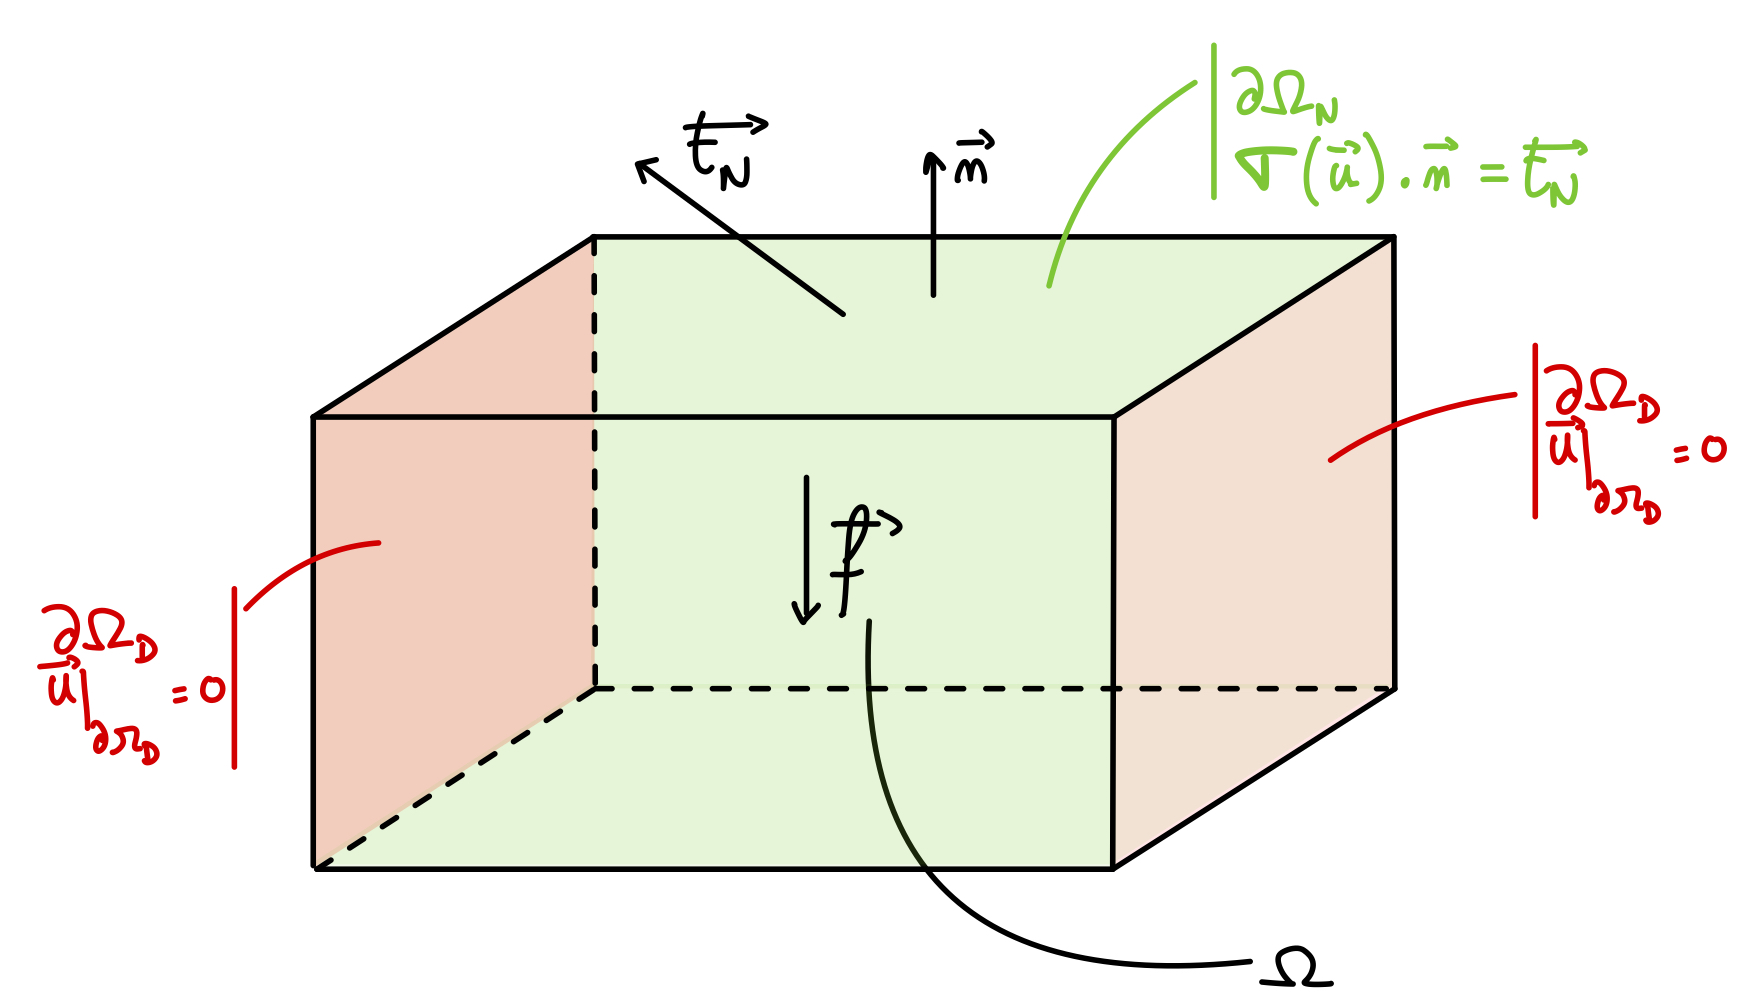
\includegraphics[width=0.61\linewidth]{figures/omega_domain}
	\caption{Representation of a domain $\Omega$}
	\label{fig:omegadomain}
\end{figure}

Let's decompose $\partial \Omega$ as $\partial \Omega_D$ and $\partial \Omega_N$ such that $\partial \Omega_D \cup \partial \Omega_N = \partial \Omega$, $\partial \Omega_D \cap \partial \Omega_N = \emptyset$. Let's denote by $\vec t_N : \partial \Omega_N \rightarrow \mtr^3$ the normal traction force and $\vec n$ the normal vector of $\partial \Omega$ outside-oriented. We can consider the boundary displacement on $\partial \Omega_D$ as equal to $\vec 0$. 

In case of non-homogeneous boundary conditions $\vec g : \partial \Omega_D \rightarrow \mtr^3$, we can solve the problem for $\vec u - \vec g$ by modifying the source term. Then, the solution of linear elasticity problem should verify :
$
\left\{ \begin{array}{ll}
\vec u = \vec 0 & \partial \Omega_D \\
\boldsymbol{\sigma} (\vec u) \cdot \vec n = \vec t_N & \partial \Omega_N
\end{array} \right.
$

Physically, $\vec f$ is a "body force" on $\Omega$ and $\vec t_N$ is a "surface traction". 
The strong formulation of this problem is : \\
For a given $\vec f \in \boldsymbol L^2(\Omega)$, $\vec t_N \in \boldsymbol L^2(\partial \Omega_N)$, find $\vec u \in \boldsymbol H^1(\Omega)$ such that : 

\begin{tcolorbox}
\begin{equation}
\label{eq:strong_form}
\left\{
\begin{aligned}
    & - \div \boldsymbol{\sigma} (\vec u) = \vec f & \text{ in } & \Omega \hspace{1cm} \text{(Equilibrium)}\\
    & \boldsymbol{\sigma} (\vec u) = \lambda (\div \vec u) I_3 + \mu (\grad \vec u + (\grad \vec u)^T) & \text{ in }& \Omega \hspace{1cm} \text{(Hooke's law)} \\
    & \vec u = \vec 0 & \text{ in } &\partial \Omega_D \\
    & \boldsymbol{\sigma} (\vec u) \cdot \vec n = \vec t_N & \text{ in }& \partial \Omega_N
\end{aligned}
\right.
\end{equation}
\end{tcolorbox}

where $\boldsymbol L^2(\Omega) = \left(L^2(\Omega) \right)^3, \boldsymbol L^2(\partial \Omega_N) = \left(L^2(\partial \Omega_N) \right)^3, \boldsymbol H^1(\Omega) = \left(H^1(\Omega) \right)^3, $

\section{Pure displacement weak-formulation} \label{sec:Pure displacement weak-formulation}

To derive the weak formulation from \eqref{eq:strong_form}, let's introduce the following functional space : $\boldsymbol H^1_{\vec 0,D}(\Omega) = \left\{ \vec v \in \boldsymbol H^1(\Omega) \Big| \vec v_{|\partial\Omega_D} = \vec 0 \right\},$
which is a sub-Hilbert space of $\boldsymbol H^1(\Omega)$ equipped with the same inner product (as a closed space of a Hilbert space). By taking the scalar product of the equilibrium equation from \eqref{eq:strong_form} with $\vec v \in \left(H^1_{\vec 0,D}(\Omega) \right)^3$ and applying a Green's formula, one obtains :
$\int_\Omega \boldsymbol{\sigma} (\vec u) : (\grad \vec v) \dif \Omega - \int_{\partial\Omega} \left(\boldsymbol{\sigma} (\vec u).\vec n \right).\vec v \dif \Gamma = \int_\Omega \vec f . \vec v \dif \Omega$

One can remark that with \eqref{eq:hooklaw}, the tensor $\boldsymbol \sigma (\vec u)$ is symmetric. It implies that : 
$\boldsymbol \sigma (\vec u) : \grad \vec v = \boldsymbol \sigma(\vec u) : \boldsymbol \varepsilon (\vec v)$
Moreover, $\vec v \in \left(H^1_{\vec 0,D}(\Omega) \right)^3$, then $\vec v_{|\partial\Omega_D} = \vec 0$. Thus, the weak formulation can be simplified to : 

\begin{tcolorbox}
\begin{equation}
\label{eq:weakdisplacementform}
\left\{
    \begin{aligned}
    &\text{Find } \vec u \in \boldsymbol H^1_{\vec 0,D}(\Omega) \text{ such that :}\\
    & a(\vec u,\vec v) = l(\vec v) \hspace{0.5cm} \forall \vec v \in \boldsymbol H^1_{\vec 0,D}(\Omega)
    \end{aligned}
\right.
\end{equation}
\end{tcolorbox}




With : 
\begin{equation*}
    \begin{aligned}
        & a : \left\{
        \begin{aligned}
            &\boldsymbol H^1_{\vec 0,D}(\Omega) \times \boldsymbol H^1_{\vec 0,D}(\Omega)  \rightarrow \mtr \\
            &(\vec u,\vec v)  \longmapsto \int_\Omega \boldsymbol \sigma(\vec u) : \boldsymbol \varepsilon (\vec v) \dif \Omega = \int_\Omega \lambda (\div \vec u) (\div \vec v) \dif \Omega+ \int_\Omega 2\mu \boldsymbol \varepsilon(\vec u): \boldsymbol \varepsilon (\vec v)\dif \Omega
        \end{aligned}
        \right. \\
    	& l : \left\{
        \begin{aligned}
            &\boldsymbol H^1_{\vec 0,D}(\Omega) \rightarrow \mtr \\
            &\vec v \longmapsto \int_\Omega \vec f . \vec v \dif \Omega + \int_{\partial\Omega_N} \vec t_N.\vec v \dif \Gamma
        \end{aligned}
        \right.
    \end{aligned}
\end{equation*}
In continuum mechanics, \eqref{eq:weakdisplacementform} is known as the Principle of Virtual Work. Let's look at the well-posedness of \eqref{eq:weakdisplacementform}. Before starting, let's recall some notations and lemmas. \\

$\norm{.}_{\boldsymbol H^1(\Omega)}$ is defined as : $\forall \vec v \in \boldsymbol H^1(\Omega), \norm{\vec v}_{\boldsymbol H^1(\Omega)} = \left(\sum_{i=1}^3 \norm{v}_{H^1(\Omega)}^2 \right)^{1/2}$. 
\begin{lemma}
\begin{enumerate}
    \item $\displaystyle \forall \vec u \in \boldsymbol H^1(\Omega)$, $\int_\Omega (\div \vec u)^2 \dif \Omega \leq 3 \norm{\vec u}_{\boldsymbol H^1(\Omega)}^2$
    \item $\displaystyle \forall \vec u \in \boldsymbol H^1(\Omega)$,$\boldsymbol \varepsilon(\vec u) : \boldsymbol \varepsilon(\vec u) \leq \grad \vec u : \grad \vec u$
    Then : $\int_\Omega \boldsymbol \varepsilon(\vec u) : \boldsymbol \varepsilon(\vec u) \dif\Omega \leq \int_\Omega \grad \vec u : \grad \vec u \dif \Omega \leq \norm{\vec u}_{\boldsymbol H^1(\Omega)}^2$
\end{enumerate}
\end{lemma}
\begin{proof}
    By direct computation, or a detailed version in \cite{cinatl_finite}
\end{proof}

\begin{lemma}
\label{Korn1}
    (First Korn's inequality) \\
    Let $\Omega \subset \mtr^3$ a domain and denotes by $\norm{\boldsymbol \varepsilon(\vec u)}_{\boldsymbol L^2(\Omega)} := \left(\int_\Omega \boldsymbol \varepsilon(\vec u):\boldsymbol \varepsilon(\vec u)\right)^{1/2}$. Then, there exists $C > 0$ such that: $\forall \vec v \in \boldsymbol H^1_{\vec 0}(\Omega), \hspace{1cm} C\norm{\vec v}_{\boldsymbol H^1(\Omega)} \leq \norm{\boldsymbol \varepsilon(\vec v)}_{\boldsymbol L^2(\Omega)}$
\end{lemma}
\begin{proof}
    A proof can be found in \cite{brenner_mathematical_2008}
\end{proof}

\begin{lemma}
\label{Korn2}
    (Second Korn's inequality) \\
    Let $\Omega \subset \mtr^3$ a domain. Then, there exists $C > 0$ such that: 
    $\forall \vec v \in \boldsymbol H^1(\Omega), \hspace{1cm} C\norm{\vec v}_{\boldsymbol H^1(\Omega)} \leq \norm{\boldsymbol \varepsilon(\vec v)}_{\boldsymbol L^2(\Omega)} + \norm{\vec v}_{\boldsymbol L^2(\Omega)}$
    By Rellich theorem, $\boldsymbol H^1(\Omega)$ is compactly embedded in $\boldsymbol L^2(\Omega)$ as $\Omega$ is a open bounded domain . Then, one can show that there exists $C > 0$ such that:
    $\forall \vec v \in \boldsymbol H^1(\Omega), \hspace{1cm} C\norm{\vec v}_{\boldsymbol H^1(\Omega)} \leq \norm{\boldsymbol \varepsilon(\vec v)}_{\boldsymbol L^2(\Omega)}$
\end{lemma}
\begin{proof}
    A proof can be found in \cite{brenner_mathematical_2008}
\end{proof}


\noindent \textbf{Now, we can prove the well-posedness of \eqref{eq:weakdisplacementform} when $\left| \Omega_D \right| > 0$.}
\begin{itemize}
    \item $\left(\boldsymbol H^1_{\vec 0,D}(\Omega), \norm{.}_{\boldsymbol H^1(\Omega)} \right)$ is a Hilbert space.
    \item $a(.,.)$ is a bilinear form on $\boldsymbol H^1_{\vec 0,D}(\Omega) \times \boldsymbol H^1_{\vec 0,D}(\Omega)$ and $l(.)$ a linear form on $\boldsymbol H^1_{\vec 0,D}(\Omega)$.
    \item $l(.)$ is continuous : \begin{equation*}
    \begin{aligned}    
    \forall \vec v \in \boldsymbol H^1_{\vec 0,D}(\Omega), \left|l(\vec v)\right| 
    & \leq \left| \left(\vec f, \vec v \right)_{\boldsymbol L^2(\Omega)} + \left(\vec t_N, \vec v \right)_{\boldsymbol L^2(\partial \Omega_N)} \right| \\
    \left|l(\vec v)\right| 
    & \leq \left( \norm{\vec f}_{\boldsymbol L^2(\Omega)} + \norm{\gamma_0} \norm{\vec t_N}_{\boldsymbol L^2(\partial \Omega_N)}\right)\norm{\vec v}_{\boldsymbol H^1(\Omega)}\\
    \end{aligned}
    \end{equation*}
	Where $\gamma_0$ is the trace operator.
    \item $a(.,.)$ is continuous: 
    \begin{equation*}
        \begin{aligned}
        \forall \vec u, \vec v \in \boldsymbol H^1_{\vec 0,D}(\Omega), \left| a(\vec u, \vec v) \right| 
        & \leq \left| a(\vec u, \vec u) \right|^{1/2} \left| a(\vec v, \vec v) \right|^{1/2} & \text{By the Cauchy-Schwarz Inequality as $a(.,.)$ is} \\
        & & \text{a symmetric and positive bilinear form} \\
        \left| a(\vec u, \vec v) \right| & \leq (3\lambda + 2\mu)\norm{\vec u}_{\boldsymbol H^1(\Omega)}\norm{\vec v}_{\boldsymbol H^1(\Omega)}.
        \end{aligned}
    \end{equation*}
    \item $a(.,.)$ is coercive: 
        \begin{itemize}
            \item If $\Omega_D = \Omega$, then $\boldsymbol H^1_{\vec 0,D}(\Omega) = \boldsymbol H^1_{\vec 0}(\Omega)$ and we can apply \textbf{Lemma \ref{Korn1}} : there exists $C > 0$ such that:
            \begin{equation*}
                \begin{aligned}
                    \forall \vec u \in \boldsymbol H^1_{\vec 0,D}(\Omega), \hspace{0.3cm} a(\vec u, \vec u) 
                    &= \int_\Omega \lambda (\div \vec u)^2 \dif \Omega + \int_\Omega 2\mu \boldsymbol \varepsilon(\vec u): \boldsymbol \varepsilon (\vec u)\dif \Omega \\
                    & \geq 2\mu \norm{\boldsymbol \varepsilon(\vec u)}_{\boldsymbol{L}^2(\Omega)} \\
                    a(\vec u, \vec u) & \geq 2\mu C \norm{\vec u}_{\boldsymbol{H}^1(\Omega)}^2
                \end{aligned}
            \end{equation*}
            \item If $\Omega_D \subsetneq \Omega$, we can now apply \textbf{Lemma \ref{Korn2}} : there exists $C >0$ such that:
            $\forall \vec u \in \boldsymbol H^1_{\vec 0,D}(\Omega), \hspace{0.3cm}a(\vec u, \vec u) \geq 2\mu C \norm{\vec u}_{\boldsymbol{H}^1(\Omega)}^2$
        \end{itemize}
\end{itemize}

Then, by Lax-Milgram theorem, the problem \eqref{eq:weakdisplacementform} is well-posed when $\left| \Omega_D \right| > 0$. \\
When, $\left| \Omega_D \right| = 0$, \eqref{eq:weakdisplacementform} turns into the\textbf{ Pure Traction Problem} : 
\begin{tcolorbox}
\begin{equation}
\label{eq:puretractionproblem}
\left\{
    \begin{aligned}
    &\text{Find } \vec u \in \boldsymbol H^1(\Omega) \text{ such that :}\\
    & a(\vec u,\vec v) = \int_\Omega \vec f . \vec v \dif \Omega + \int_{\partial\Omega} \vec t_N.\vec v \dif \Gamma =:l(\vec v) \hspace{0.5cm} \forall \vec v \in \boldsymbol H^1(\Omega)
    \end{aligned}
\right.
\end{equation}
\end{tcolorbox}

This problem is not truly well-posed. Regarding the Rigid Displacement Field (translations and rotations) $\boldsymbol{\mathcal{R}} = \left\{\vec v \in \boldsymbol H^1(\Omega) \left| \exists a, b \in \mtr^3, \vec v(x) = a + b \times x \right. \right\}$, $\forall \vec v \in \boldsymbol{\mathcal{R}}, \hspace{0.3cm} \div v = 0 \text{ and } \boldsymbol \varepsilon(\vec v) = 0.$
Then : $\forall \vec u \in \boldsymbol H^1(\Omega), \forall \vec v \in \boldsymbol{\mathcal{R}},\hspace{0.3cm} a(\vec u, \vec v)= 0.$
So, the weak formulation \eqref{eq:puretractionproblem} is solvable iff the following compatibility condition holds : $\forall \vec v \in \boldsymbol{\mathcal{R}}, \hspace{0.3cm}\int_\Omega \vec f . \vec v \dif \Omega + \int_{\partial\Omega} \vec t_N.\vec v \dif \Gamma = 0,$
and in this case, there exists an unique solution $\vec u \in \hat{\boldsymbol H}^1(\Omega) := \left\{\vec v \in \boldsymbol H^1(\Omega) \left| \displaystyle \int_\Omega \vec v \dif \Omega = \int_\Omega  \curl \vec v \dif \Omega = \vec 0 \right. \right\}$ 
In case of \textbf{Pure Traction Problem}, we are looking for a solution modulo a rigid displacement field.
\textit{A more rigorous proof of the equivalence can be found in \cite{brenner_mathematical_2008} and \cite{chen_variational}.}


\section{Numerical simulation using \texttt{PSYDAC} on the supercomputer Raven}

\texttt{PSYDAC} is a high-level programming IDE and very intuitive to use. It uses \texttt{SymPDE} and \texttt{Pyccel}. \texttt{SymPDE} implements in \texttt{Python} abstract objects (functional space, differential operators, linear and bilinear forms...). \texttt{Pyccel} is a transpiler, used to convert a \texttt{Python} code into a \texttt{C} or \texttt{Fortran} code, in order to take advantage of code acceleration and parallelization. Figure \ref{fig:Dependancy_Psydac} summarizes the dependency between \texttt{PSYDAC}, \texttt{SymPDE} and \texttt{Pyccel}. A more detailed presentation of \texttt{PSYDAC} can be found in \cite{guclu_psydac_2022}.

\begin{figure}[!h]
	\centering
	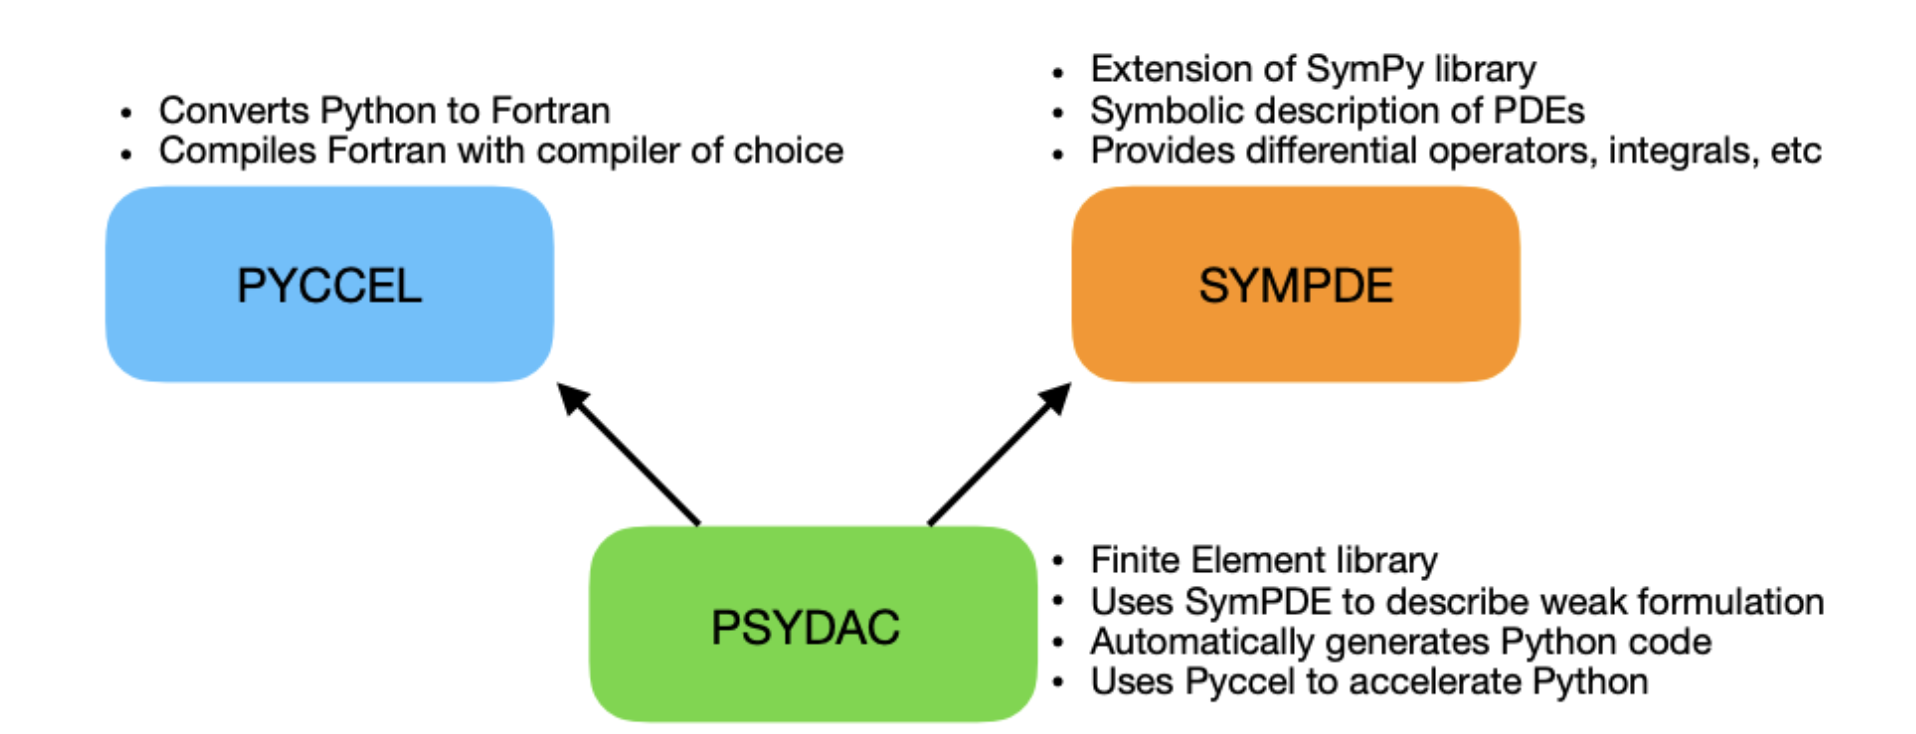
\includegraphics[width=0.75\linewidth]{figures/psydac_fonc_1.png}
	\caption{Dependency graph of \texttt{PSYDAC}, from \cite{guclu_psydac_2022}}
	\label{fig:Dependancy_Psydac}
\end{figure}

Raven is a supercomputer located at the Max-Planck Institute for Plasma Physics. It is part of the High Performance Computing (HPC) infrastructure and is used for large-scale simulations and data analysis in plasma physics and related fields. I had the opportunity to run my simulations on Raven, which provided me with access to powerful computational resources and parallel processing capabilities. 


\subsection{Dirichlet homogeneous boundary conditions on $\partial\Omega_D = \partial\Omega$} \label{subsec:Dirichlet Homogeneous Boundary conditions on}

At first, to get familiar with \texttt{PSYDAC} and the HPC, I considered the case $\Omega = [0,1]^3$, $\partial \Omega_D = \partial\Omega$ and $\partial \Omega_N = \emptyset$. To verify if the numerical resolution of \texttt{PSYDAC} of \eqref{eq:weakdisplacementform} is correct, I used the Method of Manufactured Solutions. The concept is quite simple: we assume that a function $\vec u_e \in \boldsymbol H^1_{\vec 0}(\Omega)$ verifies the strong problem \eqref{eq:strong_form}, then we compute the source term $\vec f$ and we solve \eqref{eq:weakdisplacementform} with $\vec f$ as a source term and we look at the error between the numerical solution and the theoretical one.
I considered $\vec u_e$ defined as: $\vec u_e = \begin{pmatrix}
	0 \\
	0 \\
\sin{\left(\pi x \right)} \sin{\left(\pi y \right)} \sin{\left(\pi z \right)}
\end{pmatrix} \in \boldsymbol H^1_{\vec 0}(\Omega).$ Then, we can compute manually the source term $\vec f$: $\vec f = \begin{pmatrix}
	 - \pi^{2} \left(\lambda + \mu\right) \cos{\left(\pi x \right)} \sin{\left(\pi y \right)}  \cos{\left(\pi z \right)} \\
	 - \pi^{2} \left(\lambda + \mu\right) \sin{\left(\pi x \right)} \cos{\left(\pi y \right)} \cos{\left(\pi z \right)} \\
	  \pi^{2} \left(\lambda + 4 \mu\right) \sin{\left(\pi x \right)} \sin{\left(\pi y \right)} \sin{\left(\pi z \right)}
\end{pmatrix} \in \boldsymbol L^2(\Omega).$

To make the numerical simulation with \texttt{PSYDAC}, we have to choose two important parameters: $d$ the maximum degree of B-spline functions that will approximate the solution and $n_{\text{cells}}$ is the number of cells in each dimension of $\Omega$ for the finite dimensional space. $\displaystyle h \propto \frac{1}{n_{\text{cells}}}$, a usual discretization parameter for finite dimensional spaces and $d$ will control the convergence speed of the numerical solution. 
The code in Section \ref{sec:lin_elas_dirichlet} presents the implementation details of the linear elasticity problem with Dirichlet boundary conditions.
By solving the problem with Dirichlet homogeneous boundary conditions on the whole boundary, one can observe the following plots of the simulated $\vec u_{e,3}^h$ for different planes $z$. It is also possible to plot the error $\vec u_{e,3} - \vec u_{e,3}^h$.
\begin{figure}[!h]
	\centering
	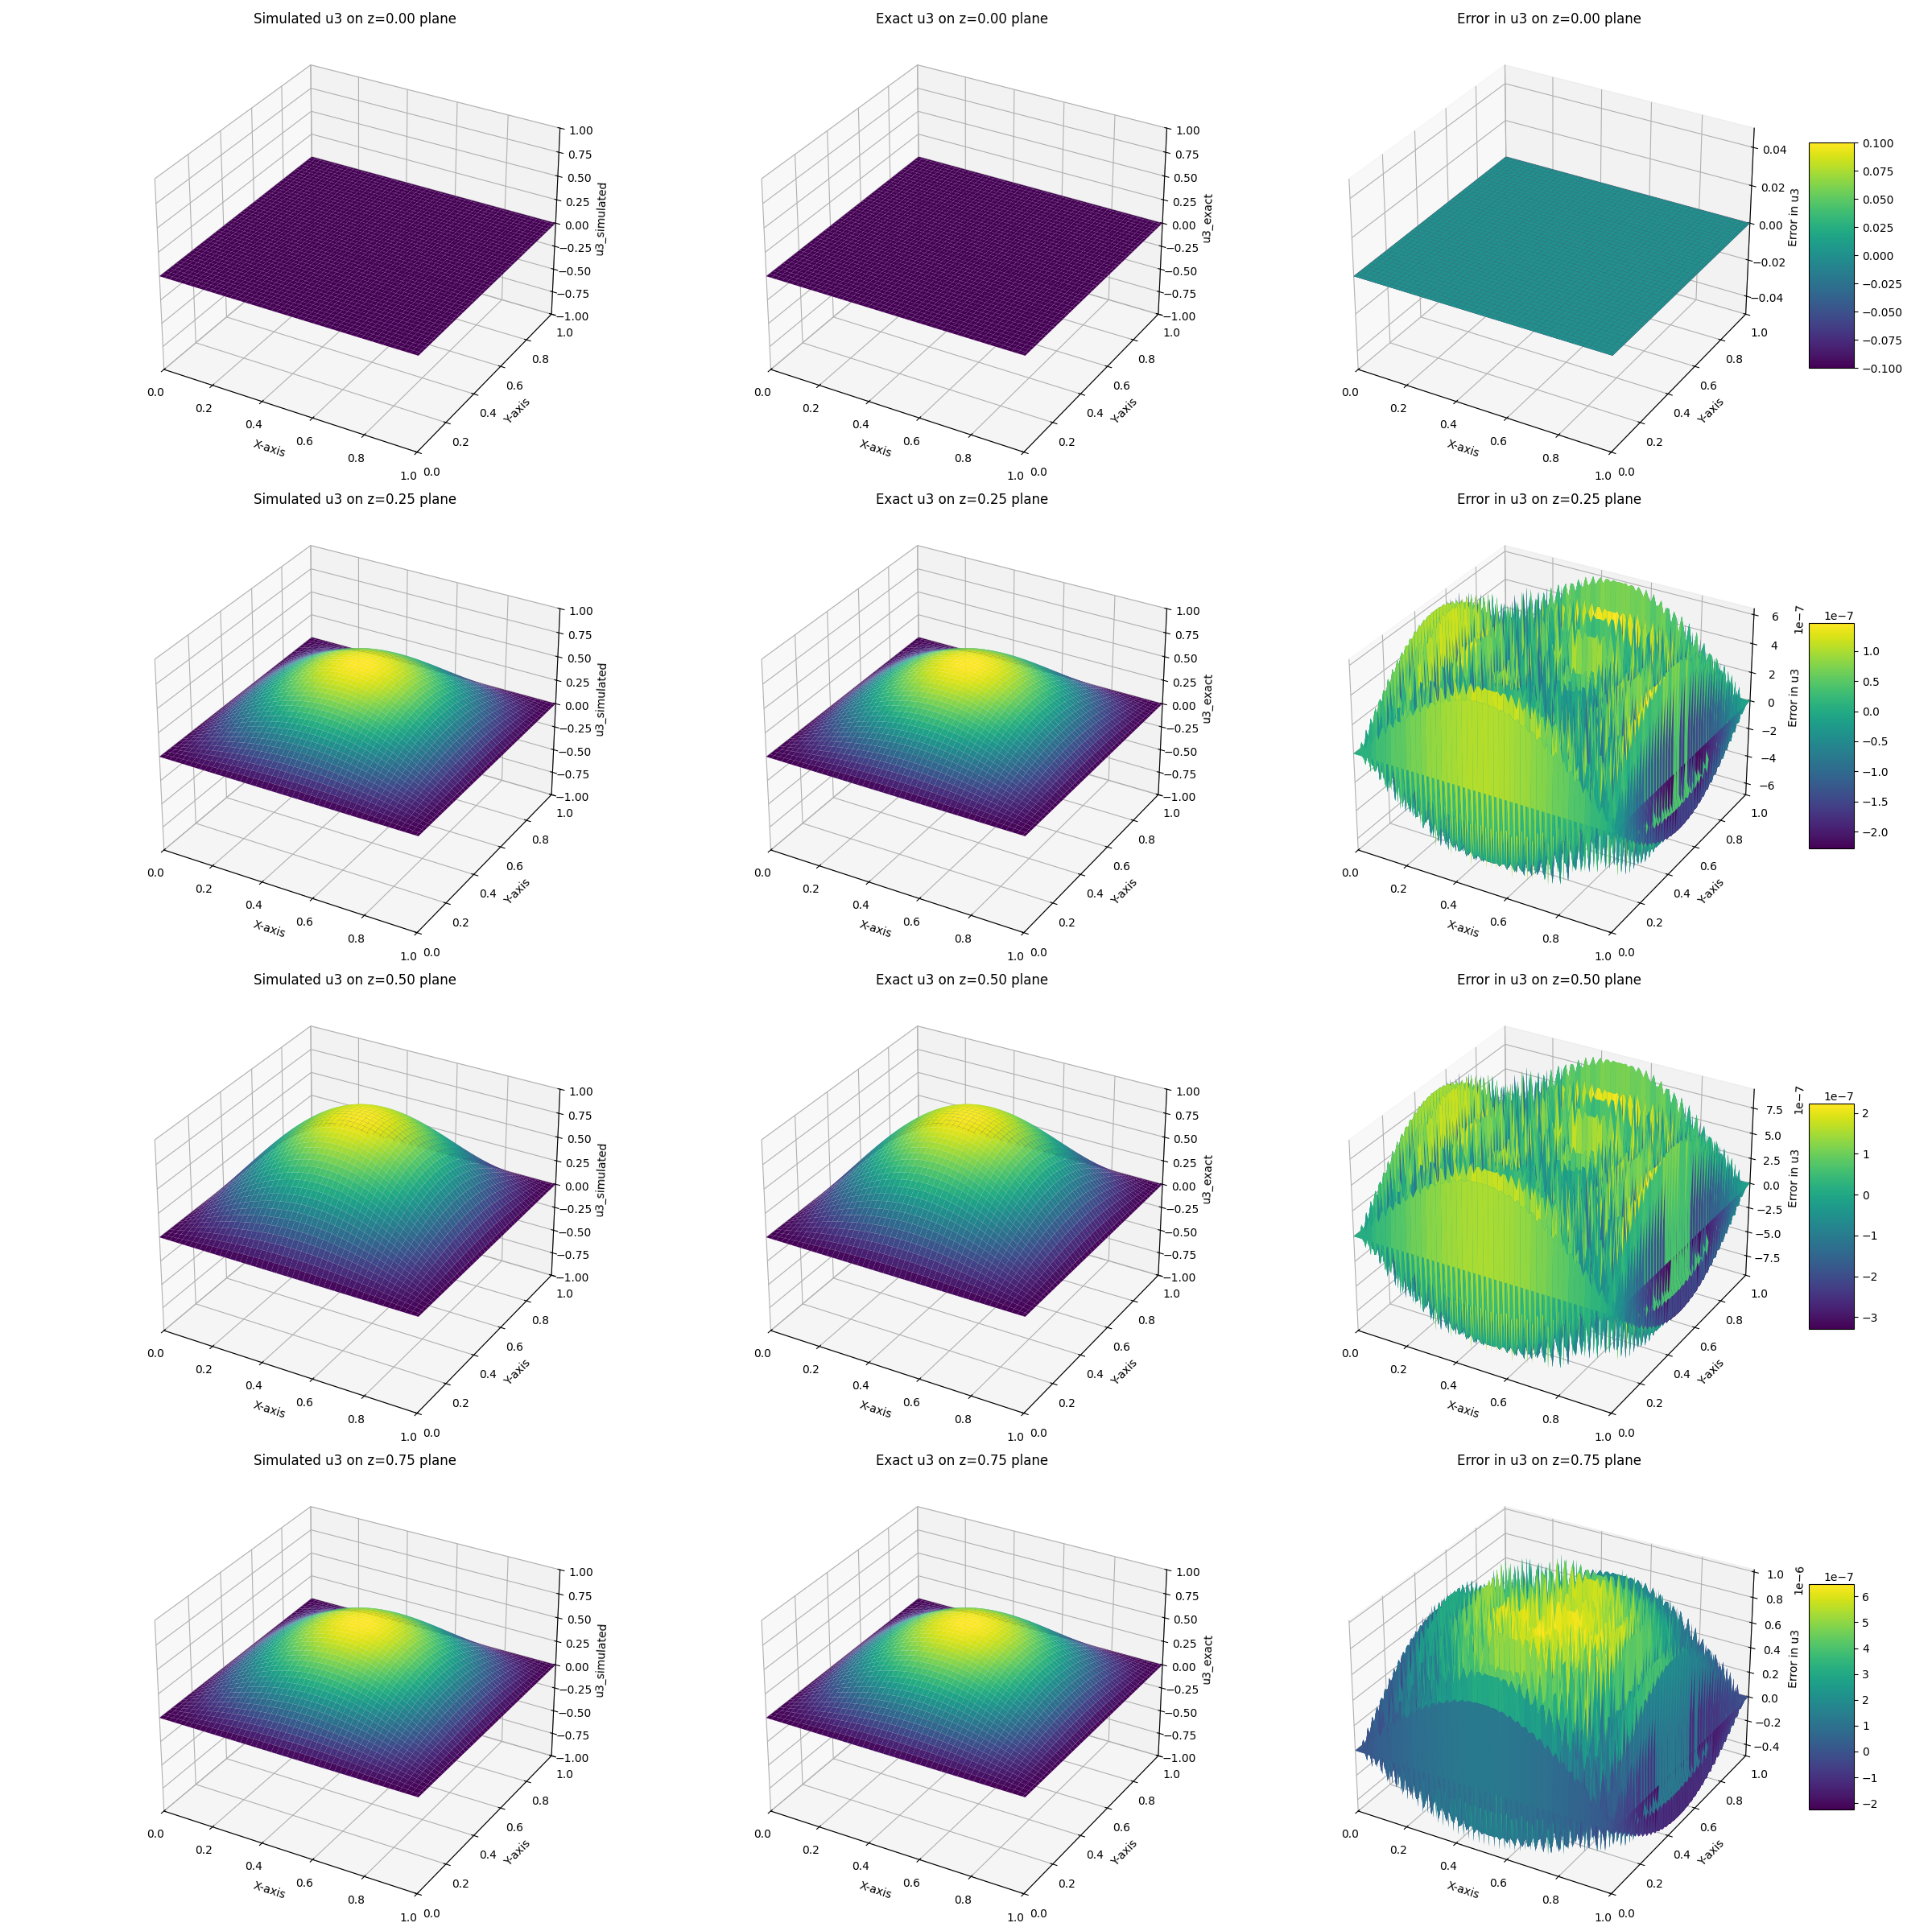
\includegraphics[width=0.8\linewidth]{figures/3d_plots_degree_2_non_mixed_dirichlet_homogeneous_ncell=64.png}
	\caption{Plots comparison between the simulated and real $u_{e,3}$ with the error, for different planes $z$, with $d=2$ and $n_{\text{cell}} = 64$}
	\label{fig:3D_plots}
\end{figure}

We can observe that the numerical solution is quite close to the real solution. To get a better estimation of the convergence rate, let's look at Céa's lemma in this case.

Let $\boldsymbol V^h \subset \boldsymbol H^1(\Omega)$ be the discrete finite dimensional space, $\vec u \in \boldsymbol H^{s+1}(\Omega) \subset \boldsymbol H^1(\Omega), 1 \leq s \leq d+1$ the real solution and $\vec u^h \in \boldsymbol V^h$ the discrete solution.
Then, Céa's lemma gives the following estimates: 
$\norm{\vec u - \vec u^h}_{\boldsymbol H^1(\Omega)} \leq \frac{3\lambda + 2\mu}{2\mu C} \inf_{\vec v^h \in \boldsymbol H^1(\Omega)} \norm{\vec u - \vec v^h}_{\boldsymbol H^1(\Omega)}$
\textit{where $C > 0$ is a constant from Korn's inequality (independent of $h$).}
By applying \textbf{Corollary 4.21, 4.27}, \textbf{Theorem 6.2} from \cite{da_veiga_mathematical_2014} and the Aubin-Nitsche theorem, we can get the following estimates: 
\begin{equation}
\begin{aligned}
& \norm{\vec u - \vec u^h}_{\boldsymbol H^1(\Omega)} \lesssim \frac{3\lambda + 2\mu}{2\mu C} h^q \norm{\vec u}_{\boldsymbol H^{q+1}(\Omega)} \\
& \norm{\vec u - \vec u^h}_{\boldsymbol L^2(\Omega)} \lesssim (3\lambda + 2\mu) h^{q+1}\norm{\vec u}_{\boldsymbol H^{q+1}(\Omega)}
\end{aligned}
\label{eq:convergence_estimates}
\end{equation}
\textit{where $q = \min{(s,d)}$}. In this case, $u_e$ is an infinitely smooth solution, then $q = d$. 

\begin{figure}[!h]
	\centering
	\begin{subfigure}[b]{0.49\textwidth}
		\centering
		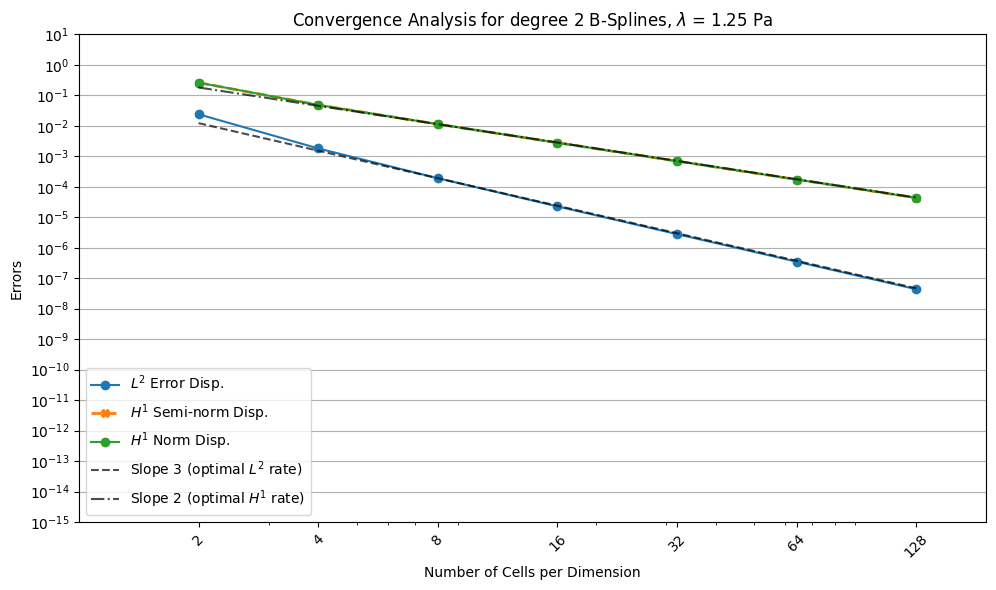
\includegraphics[width=\textwidth]{figures/figures_non_mixed_DH/convergence_plot_degree_2_lambda=1.25.png}
		\caption{$d=2$}
		\label{fig:deg2_NMDHBC}
	\end{subfigure}
	\begin{subfigure}[b]{0.49\textwidth}
		\centering
		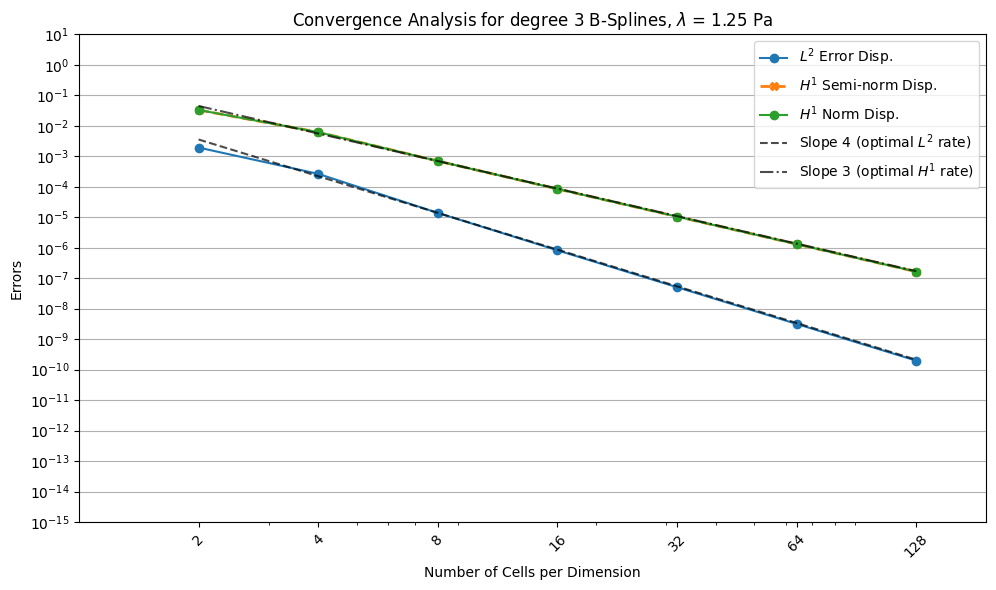
\includegraphics[width=\textwidth]{figures/figures_non_mixed_DH/convergence_plot_degree_3_lambda=1.25.png}
		\caption{$d=3$}
		\label{fig:deg3_NMDHBC}
	\end{subfigure}
	\\
	\begin{subfigure}[b]{0.49\textwidth}
		\centering
		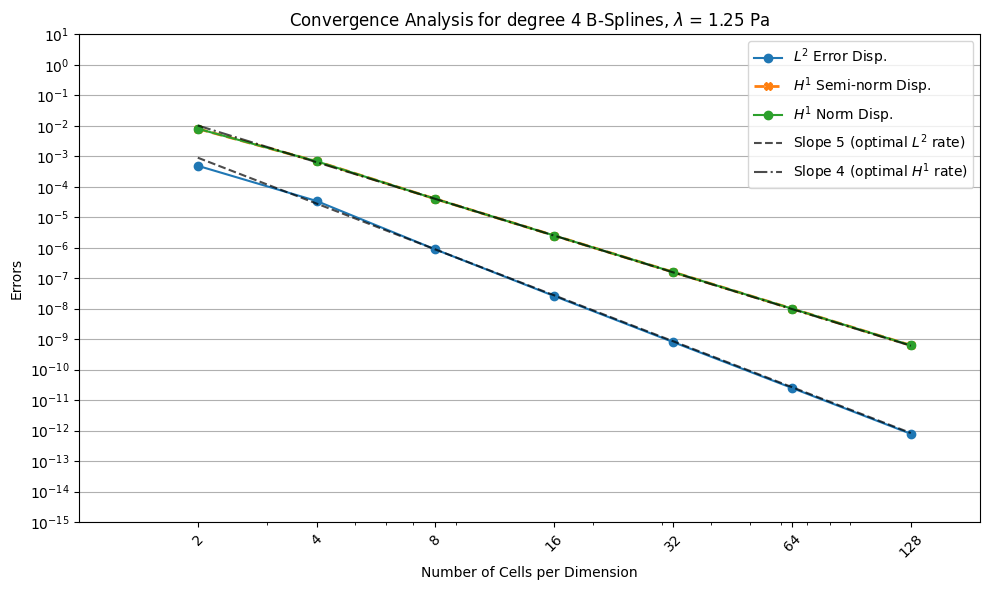
\includegraphics[width=\textwidth]{figures/figures_non_mixed_DH/convergence_plot_degree_4_lambda=1.25.png}
		\caption{$d=4$}
		\label{fig:deg4_NMDHBC}
	\end{subfigure}
	\begin{subfigure}[b]{0.49\textwidth}
		\centering
		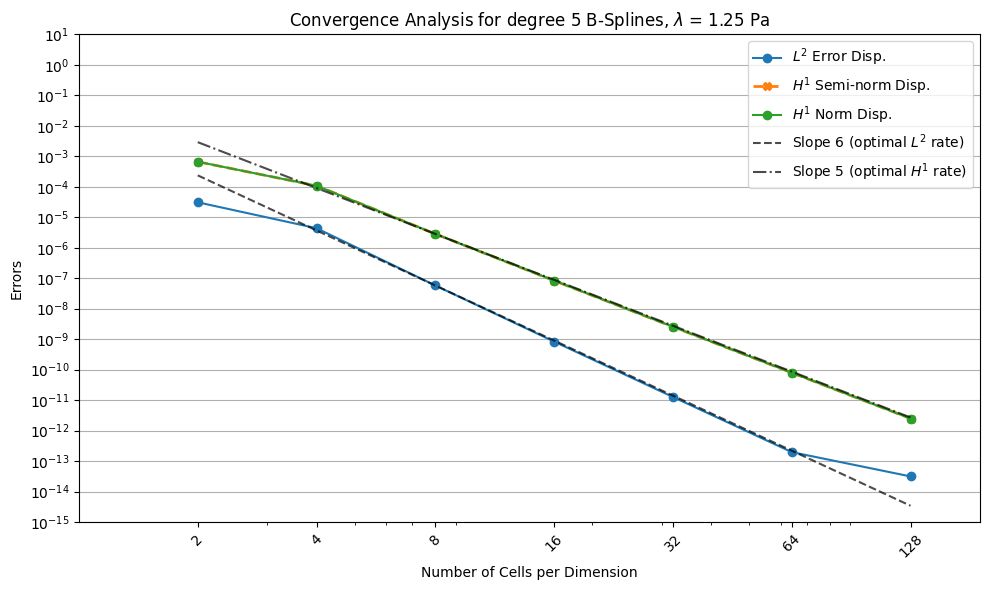
\includegraphics[width=\textwidth]{figures/figures_non_mixed_DH/convergence_plot_degree_5_lambda=1.25.png}
		\caption{$d=5$}
		\label{fig:deg5_NMDHBC}
	\end{subfigure}
	\caption{Four plots of absolute errors ($\norm{\vec u - \vec u^h}_{\boldsymbol H^1(\Omega)}$ and $\norm{\vec u - \vec u^h}_{\boldsymbol L^2(\Omega)}$) with different degree B-splines (with $\lambda = 1.25$ and $\mu = 1$)}
	\label{fig:four_errors_graphs_1}
\end{figure}

We can see that the numerical solution converges with the expected order to the real solution: the more the mesh is refined, the lower the error is, and the higher the spline degree is, the higher the convergence rate is. 
For this numerical resolution, I used the \textbf{GMRES} method to solve the linear system at the end of the discretization. This required taking care of the solver tolerance, because with a fixed tolerance, if $d$ and $n_{\text{cells}}$ are "too high", the convergence rate cannot hold. The following figure illustrates this case, when $d=5$ and $n_{\text{cells}} = 16$.

\newpage
\begin{figure}[!h]
	\centering
	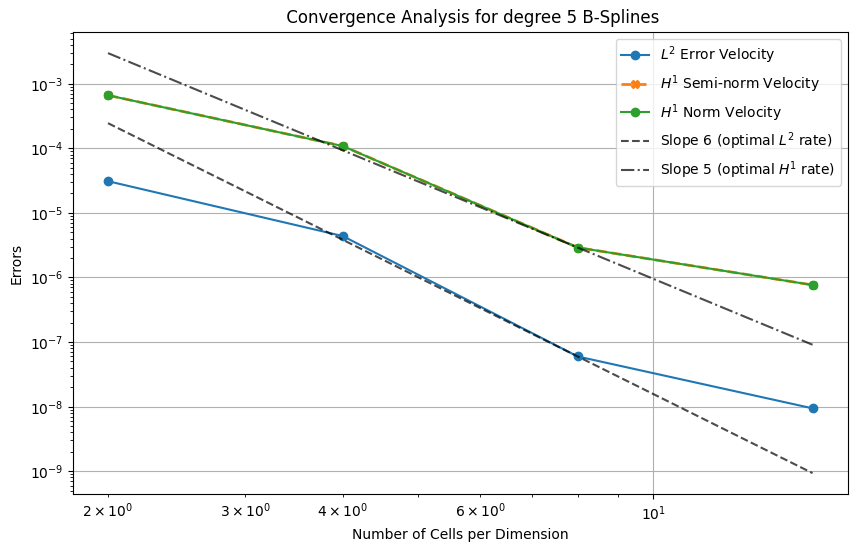
\includegraphics[width=0.7\linewidth]{figures/degre5_nul}
	\caption{Error plot between exact and numerical solution with degree 5 B-splines with "high" tolerance for the solver}
\end{figure}

But even with a lower tolerance for the solver ($10^{-15}$ for figure \ref{fig:deg5_NMDHBC}), the error reaches a plateau, which is not the case for lower degree B-splines (at least for the tested configurations). This plateau can be explained by the matrix of the bilinear form $a(.,.)$ which is ill-conditioned. Moreover, the bad conditioning can become worse with more refined mesh and higher degree B-splines (as the convergence is faster). Consequently, the iterative solver stops when the maximum number of iterations is reached (the default value is $3000$ iterations).

\subsection{Mixed boundary conditions}
\label{sec:mixed_BC}

Then, I made a simulation with mixed boundary conditions, as introduced in \eqref{eq:strong_form}, with also non-homogeneous Dirichlet boundary conditions.

Again, $\Omega = [0,1]^3$, with: 
\begin{equation*}
	\begin{aligned}
		& \partial \Omega_{\text{DH}} = \left\{  (x,y,z) \in \partial\Omega \left| z = 0 \text{ or } z = 1 \right.  \right\} \hspace{0.5cm} 
		\partial \Omega_{\text{DNH}} = \left\{  (x,y,z) \in \partial\Omega \left| x = 0 \text{ or } x = 1 \right.  \right\} \\
		& \partial \Omega_{\text{N}} = \left\{  (x,y,z) \in \partial\Omega \left| y = 0 \text{ or } y = 1 \right.  \right\}
	\end{aligned}
\end{equation*}
For that purpose, $\vec u_e, \vec f, \vec t_N$ and $\vec g$ are now defined as: 
\begin{equation*}
\begin{aligned}
	& \vec u_e =
	\begin{pmatrix}
		0 \\
		0 \\
		\sin{\left(\pi z \right)} \cos{\left(\pi x \right)} \cos{\left(\pi y \right)}
	\end{pmatrix}, \hfill \vec f =  \begin{pmatrix}
	\pi^{2} \left(\lambda + \mu\right) \sin{\left(\pi x \right)} \cos{\left(\pi y \right)} \cos{\left(\pi z \right)} \\
	\pi^{2} \left(\lambda + \mu\right) \sin{\left(\pi y \right)} \cos{\left(\pi x \right)} \cos{\left(\pi z \right)} \\
	\pi^{2} \left(\lambda + 4 \mu\right) \sin{\left(\pi z \right)} \cos{\left(\pi x \right)} \cos{\left(\pi y \right)}
	\end{pmatrix} \\
	& \vec t_N = \begin{pmatrix}
	0 \\
	- \lambda \pi \cos{\left(\pi x \right)} \cos{\left(\pi z \right)} \\
	0
	\end{pmatrix}, \hfill \vec g = \begin{pmatrix}
	0 \\
	0 \\
	\pm \sin{\left(\pi z \right)} \cos{\left(\pi y \right)}
	\end{pmatrix}
\end{aligned}
\end{equation*} 	

Then, we can get the same plots and interpretation as before in figure \ref{fig:four_errors_graphs}. 


\begin{figure}[!h]
	\centering
	\begin{subfigure}[b]{0.49\textwidth}
		\centering
		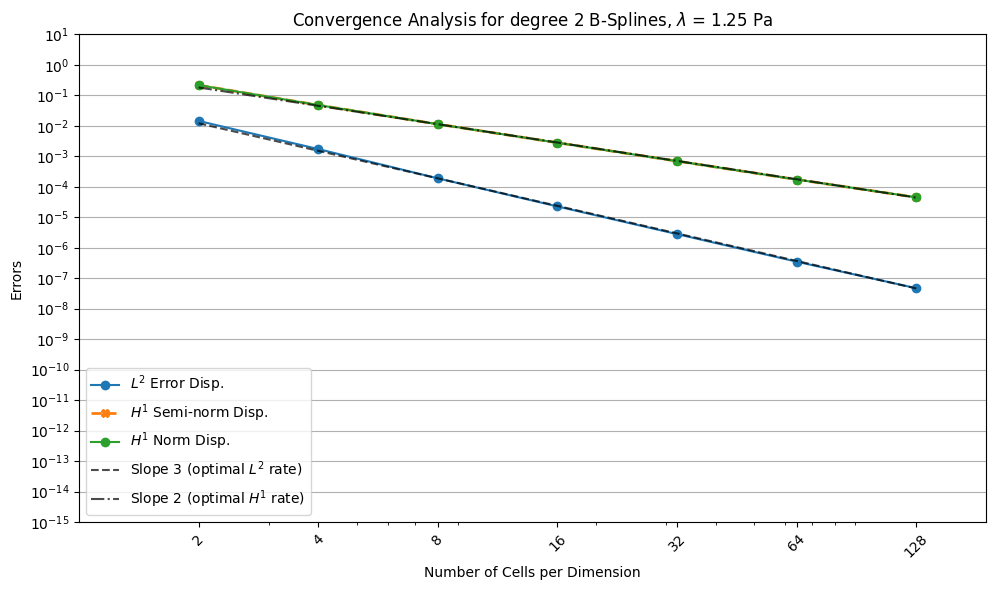
\includegraphics[width=\textwidth]{figures/figures_non_mixed/convergence_plot_degree_2_lambda=1.25.png}
		\caption{$d=2$}
		\label{fig:deg2_NM}
	\end{subfigure}
	\begin{subfigure}[b]{0.49\textwidth}
		\centering
		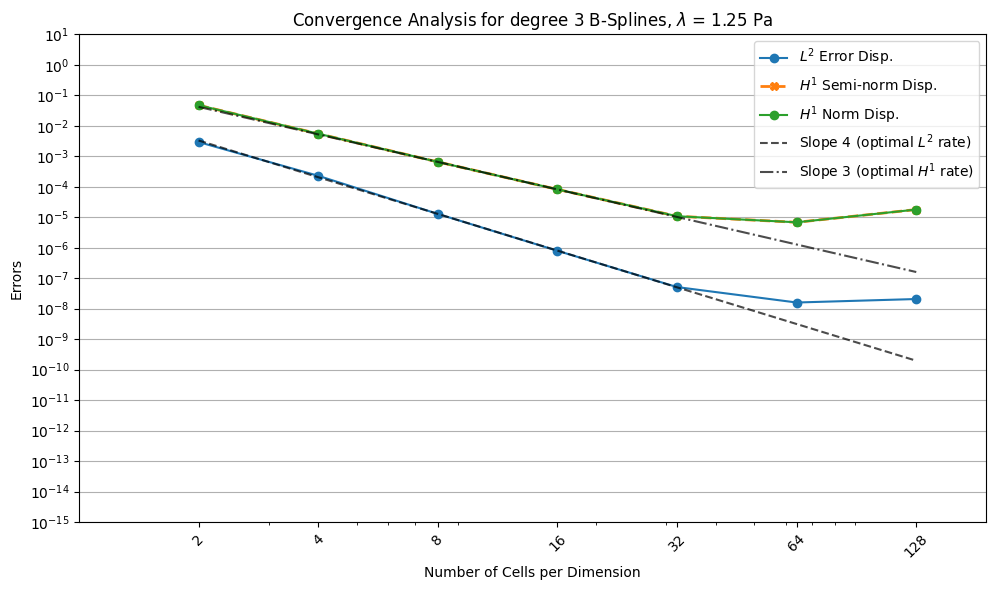
\includegraphics[width=\textwidth]{figures/figures_non_mixed/convergence_plot_degree_3_lambda=1.25.png}
		\caption{$d=3$}
		\label{fig:deg3_NM}
	\end{subfigure}
	\begin{subfigure}[b]{0.49\textwidth}
		\centering
		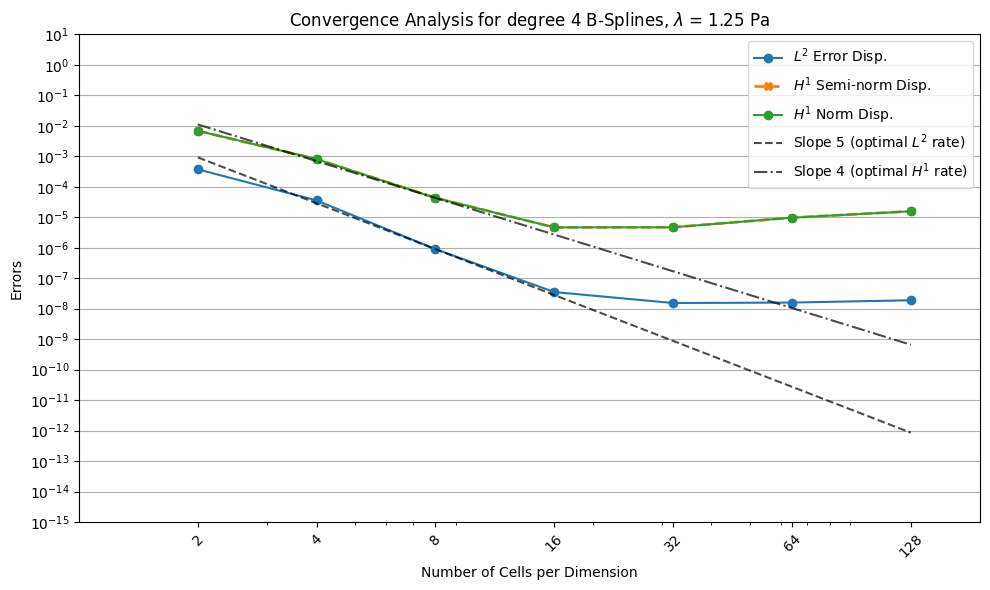
\includegraphics[width=\textwidth]{figures/figures_non_mixed/convergence_plot_degree_4_lambda=1.25.png}
		\caption{$d=4$}
		\label{fig:deg4_NM}
	\end{subfigure}
	\begin{subfigure}[b]{0.49\textwidth}
		\centering
		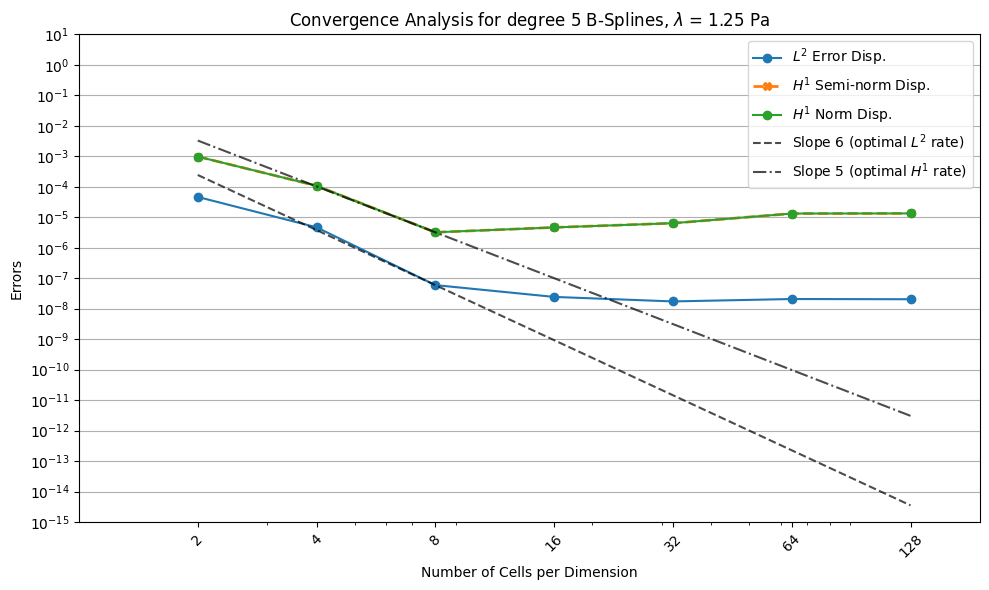
\includegraphics[width=\textwidth]{figures/figures_non_mixed/convergence_plot_degree_5_lambda=1.25.png}
		\caption{$d=5$}
		\label{fig:deg5_NM}
	\end{subfigure}
	\caption{Four plots of absolute errors ($\norm{\vec u - \vec u^h}_{\boldsymbol H^1(\Omega)}$ and $\norm{\vec u - \vec u^h}_{\boldsymbol L^2(\Omega)}$) with different degree B-splines (with $\lambda = 1.25$~Pa and $\mu = 1$~Pa)}
	\label{fig:four_errors_graphs}
\end{figure}

For fixed values $\lambda = 1.25$ and $\mu = 1$, the code seems to give a numerical solution that converges to the theoretical one with the expected order. We can notice that the plateau effect comes back and appears faster than in the case of Dirichlet homogeneous boundary conditions. The $L^2$ error seems to converge to a value slightly higher than $10^{-8}$, while the $H^1$ error converges to a value slightly higher than $10^{-5}$, and this phenomenon is more pronounced for higher degree B-splines. The limit value of each error seems to be the same for all degree B-splines, when the $L^2$ error becomes lower than $10^{-7}$ and the $H^1$ error becomes lower than $10^{-5}$. So, this plateau effect is not due to the degree of B-splines, but rather to the ill-conditioning of the matrix of the bilinear form $a(.,.)$. This ill-conditioning becomes worse with the refinement of the mesh and the increase of the degree of B-splines. A way to verify this hypothesis is to solve the linear system with a preconditioner applied to the matrices before the resolution and see if the maximum number of iterations is reached.

These simulations have been made with $\lambda = 1.25$ and $\mu = 1$. We can now look at them for more realistic values of $\lambda$ and $\mu$. The following table \ref{tab:lame_coefficients} gives the Lamé coefficients for different materials. 
\begin{table}[h]
\centering
\begin{tabular}{|c|c|c|}
\hline
Material & $\lambda$ (GPa) & $\mu$ (GPa) \\
\hline
Steel & 120 & 80 \\
\hline
Concrete & 17 & 14 \\
\hline
Rubber & 0.16 & 0.00033 \\
\hline
\end{tabular}
\caption{Lamé coefficients for different materials}
\label{tab:lame_coefficients}
\end{table}

\begin{figure}[!h]
	\centering
	\begin{subfigure}[b]{0.49\textwidth}
		\centering
		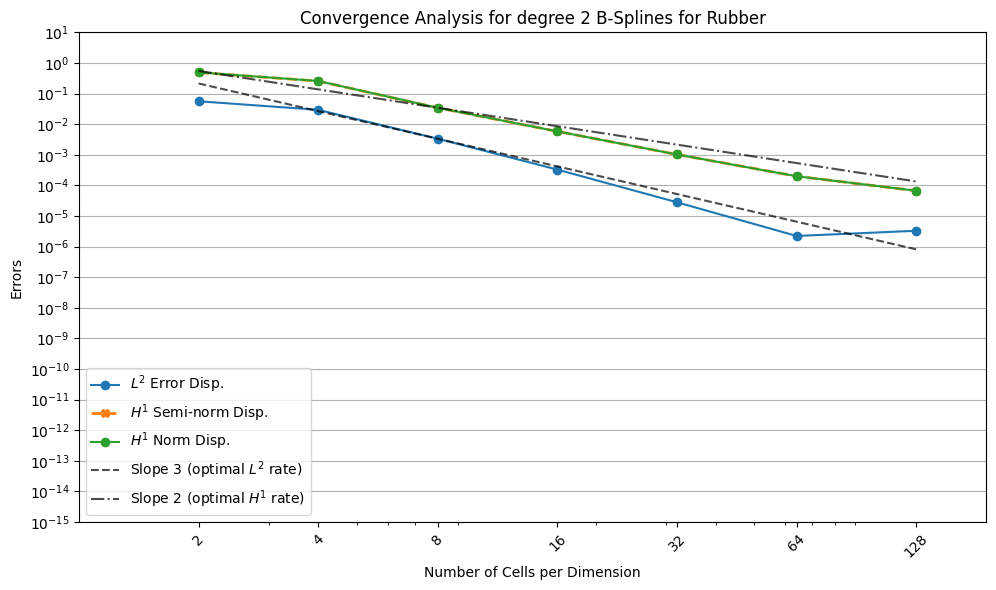
\includegraphics[width=\textwidth]{figures/figures_non_mixed_realistic/convergence_plot_degree_2_lambda=160000000.0.png}
		\caption{Rubber with degree 2 B-splines}
		\label{fig:rubber_degree_2}
	\end{subfigure}
	\begin{subfigure}[b]{0.49\textwidth}
		\centering
		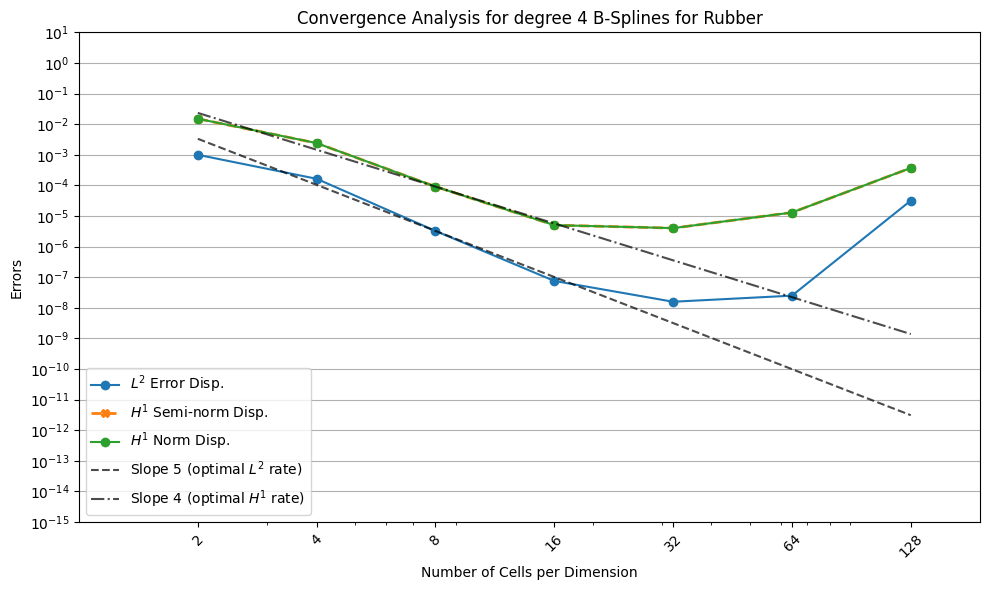
\includegraphics[width=\textwidth]{figures/figures_non_mixed_realistic/convergence_plot_degree_4_lambda=160000000.0.png}
		\caption{Rubber with degree 4 B-splines}
		\label{fig:rubber_degree_4}
	\end{subfigure}
	\centering
	\begin{subfigure}[b]{0.49\textwidth}
		\centering
		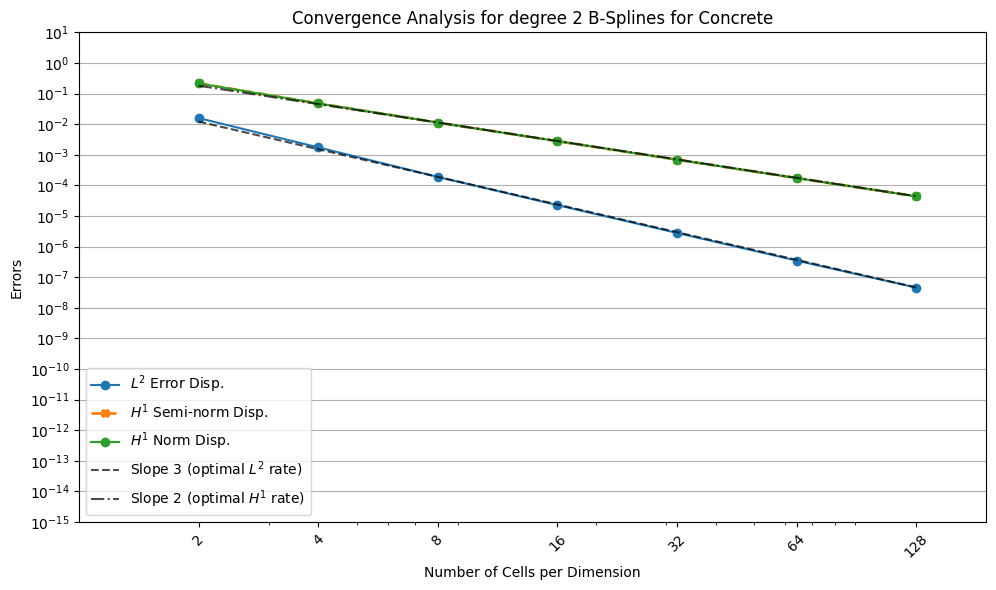
\includegraphics[width=\textwidth]{figures/figures_non_mixed_realistic/convergence_plot_degree_2_lambda=17000000000.0.png}
		\caption{Concrete with degree 2 B-splines}
		\label{fig:concrete_degree_2}
	\end{subfigure}
	\begin{subfigure}[b]{0.49\textwidth}
		\centering
		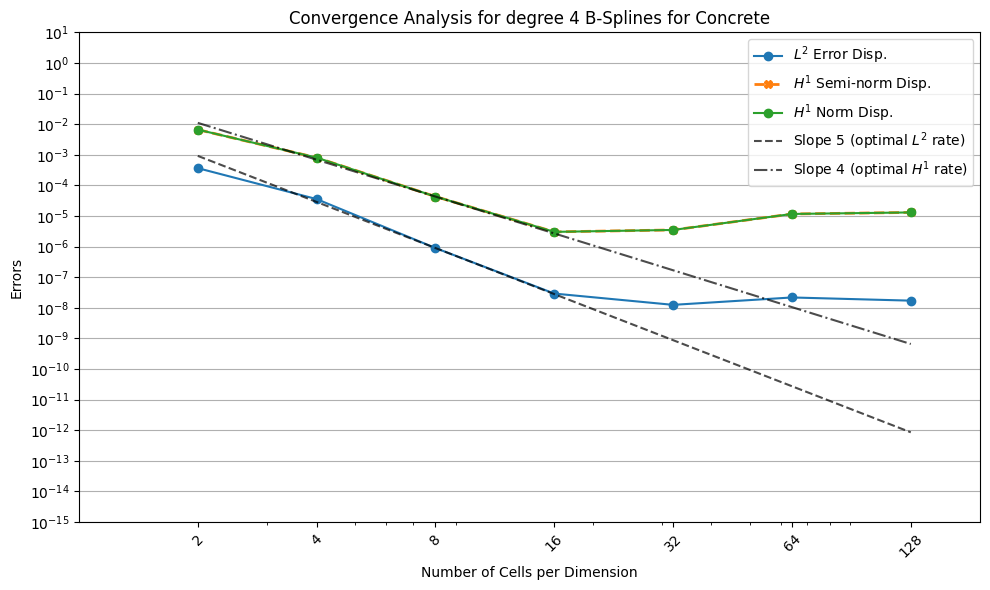
\includegraphics[width=\textwidth]{figures/figures_non_mixed_realistic/convergence_plot_degree_4_lambda=17000000000.0.png}
		\caption{Concrete with degree 4 B-splines}
		\label{fig:concrete_degree_4}
	\end{subfigure}
	\centering
	\begin{subfigure}[b]{0.49\textwidth}
		\centering
		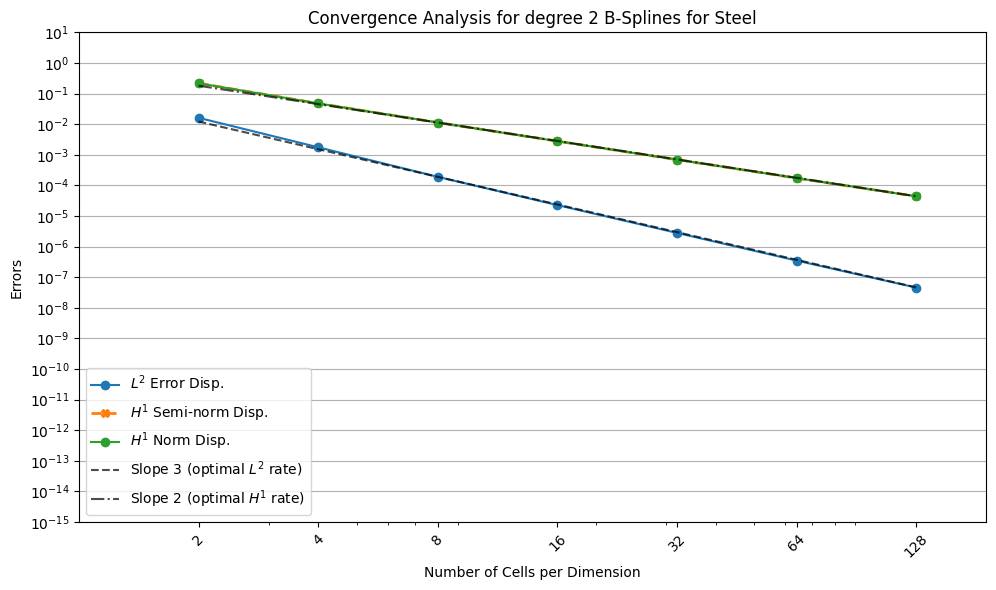
\includegraphics[width=\textwidth]{figures/figures_non_mixed_realistic/convergence_plot_degree_2_lambda=120000000000.0.png}
		\caption{Steel with degree 2 B-splines}
		\label{fig:steel_degree_2}
	\end{subfigure}
	\begin{subfigure}[b]{0.49\textwidth}
		\centering
		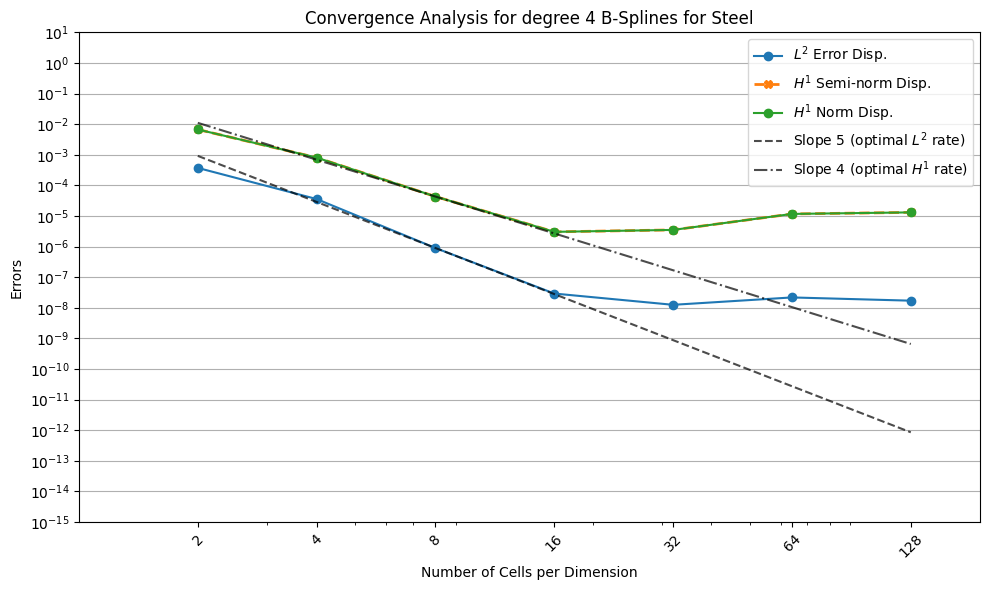
\includegraphics[width=\textwidth]{figures/figures_non_mixed_realistic/convergence_plot_degree_4_lambda=120000000000.0.png}
		\caption{Steel with degree 4 B-splines}
		\label{fig:steel_degree_4}
	\end{subfigure}
	\caption{Error plots between exact solution and numerical solution with realistic values of Lamé coefficients with degree 2 and 4 B-splines}
	\label{fig:error_realistic_lame}
\end{figure}

As we can see in figure \ref{fig:error_realistic_lame}, in the case of concrete and steel, the errors behave as expected: good convergence with expected order and the plateau effect appears after a certain value of the error. 
But for rubber, the convergence order is not really respected, the error decreases faster than expected and the plateau degenerates... 
To explain this, we can look at the estimates \eqref{eq:convergence_estimates}:
$\norm{\vec u - \vec u^h}_{\boldsymbol H^1(\Omega)} \lesssim \frac{3\lambda + 2\mu}{2\mu C} h^d \norm{\vec u}_{\boldsymbol H^{d+1}(\Omega)}$
As $\lambda$ is very high compared to $\mu$, the estimates are not really valid anymore, as $\frac{3\lambda + 2\mu}{2\mu C} \rightarrow + \infty$ when $\lambda \rightarrow + \infty$. 
This is the case for incompressible materials, like rubber, where $\lambda$ is very high compared to $\mu$. To get a better idea of the convergence, we can look at the error plots for different values of $\lambda$ with $\mu = 1$.

\begin{figure}
	\centering
	\begin{subfigure}[b]{0.49\textwidth}
		\centering
		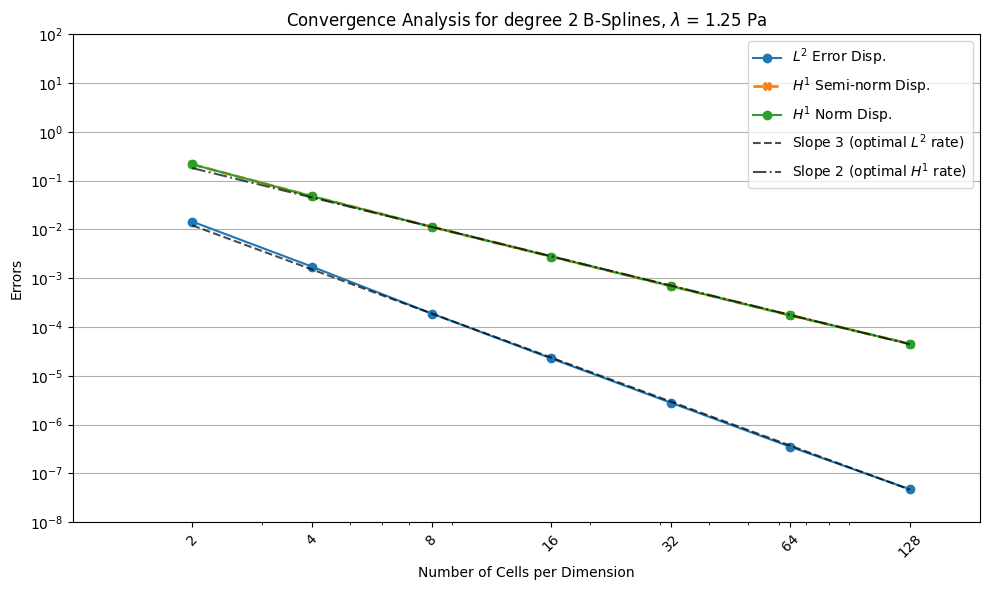
\includegraphics[width=\textwidth]{figures/figures_increasing_lambda_non_mixed/convergence_plot_degree_2_lambda=1.25.png}
		\caption{$\lambda=1.25$~Pa}
	\end{subfigure}
	\begin{subfigure}[b]{0.49\textwidth}
		\centering
		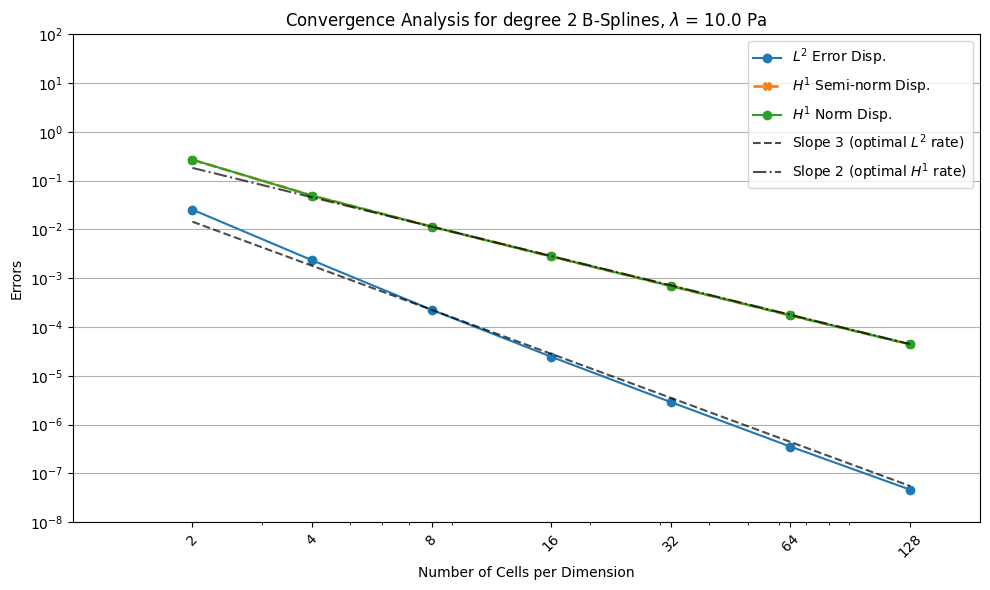
\includegraphics[width=\textwidth]{figures/figures_increasing_lambda_non_mixed/convergence_plot_degree_2_lambda=10.0.png}
		\caption{$\lambda=10$~Pa}
	\end{subfigure}
	\centering
	\begin{subfigure}[b]{0.49\textwidth}
		\centering
		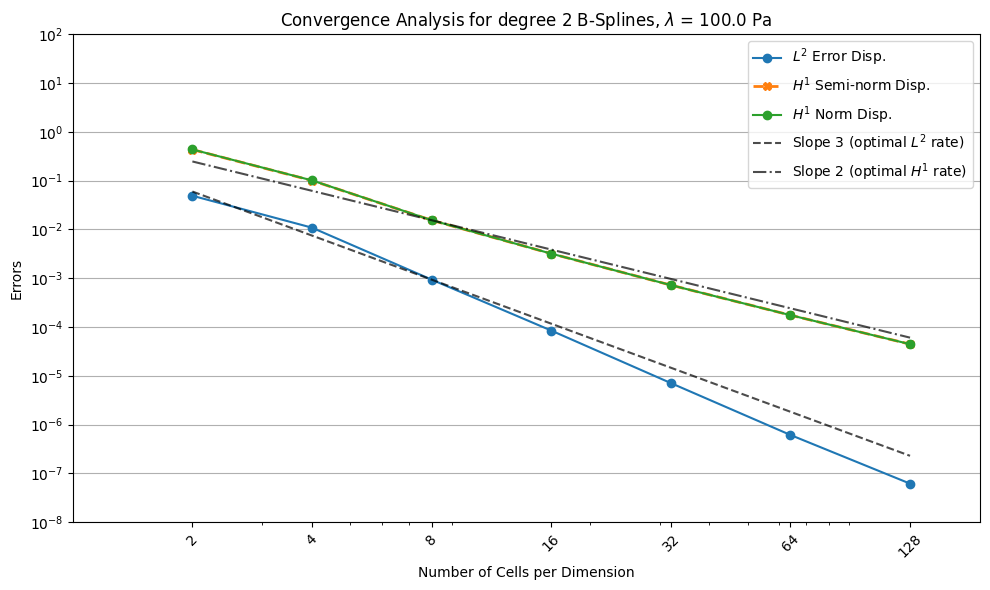
\includegraphics[width=\textwidth]{figures/figures_increasing_lambda_non_mixed/convergence_plot_degree_2_lambda=100.0.png}
		\caption{$\lambda=100$~Pa}
	\end{subfigure}
	\begin{subfigure}[b]{0.49\textwidth}
		\centering
		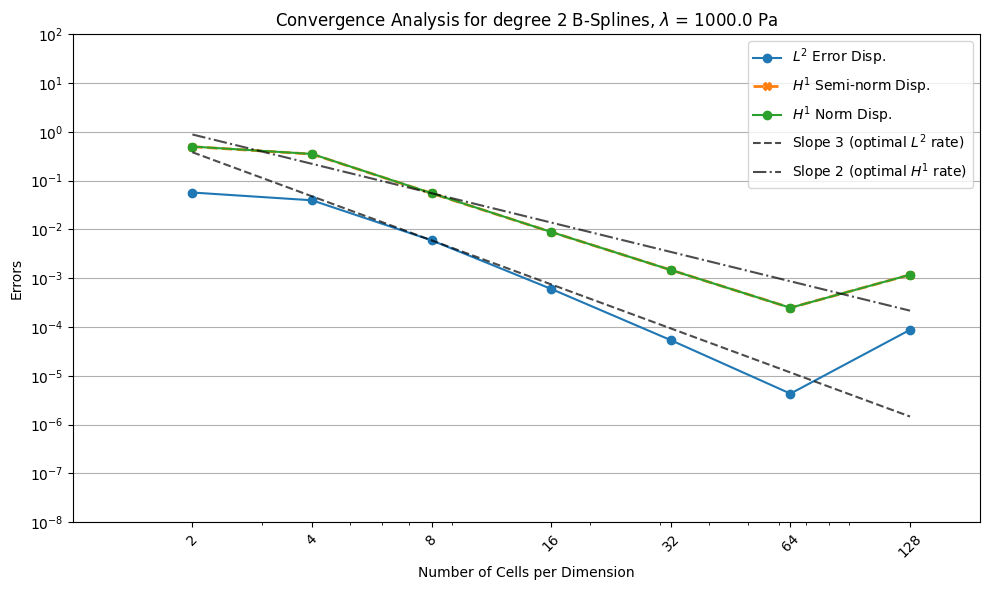
\includegraphics[width=\textwidth]{figures/figures_increasing_lambda_non_mixed/convergence_plot_degree_2_lambda=1000.0.png}
		\caption{$\lambda=1000$~Pa}
	\end{subfigure}
	\\
	\begin{subfigure}[b]{0.49\textwidth}
		\centering
		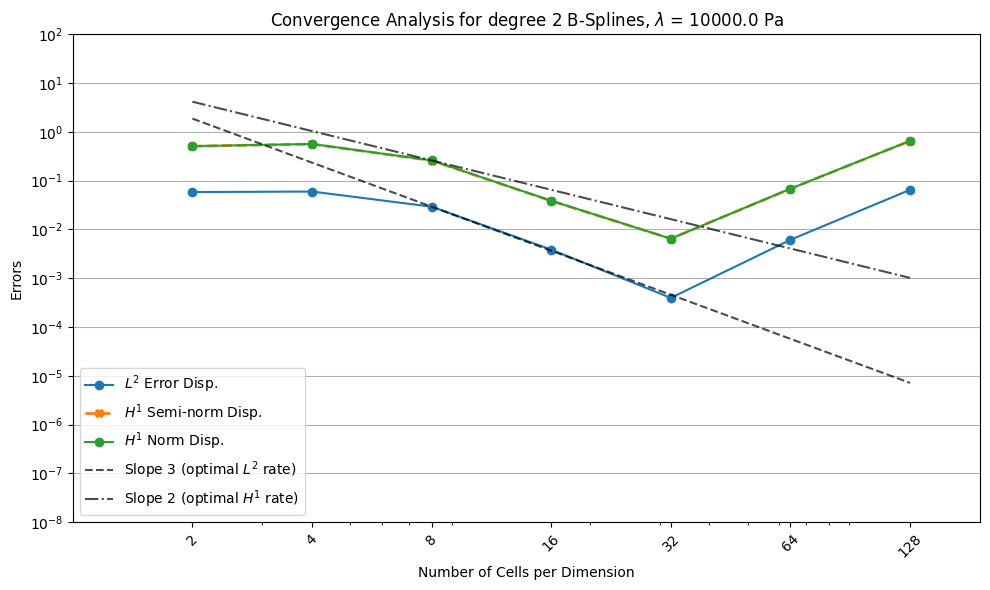
\includegraphics[width=\textwidth]{figures/figures_increasing_lambda_non_mixed/convergence_plot_degree_2_lambda=10000.0.png}
		\caption{$\lambda=10000$~Pa}
	\end{subfigure}
	\begin{subfigure}[b]{0.49\textwidth}
		\centering
		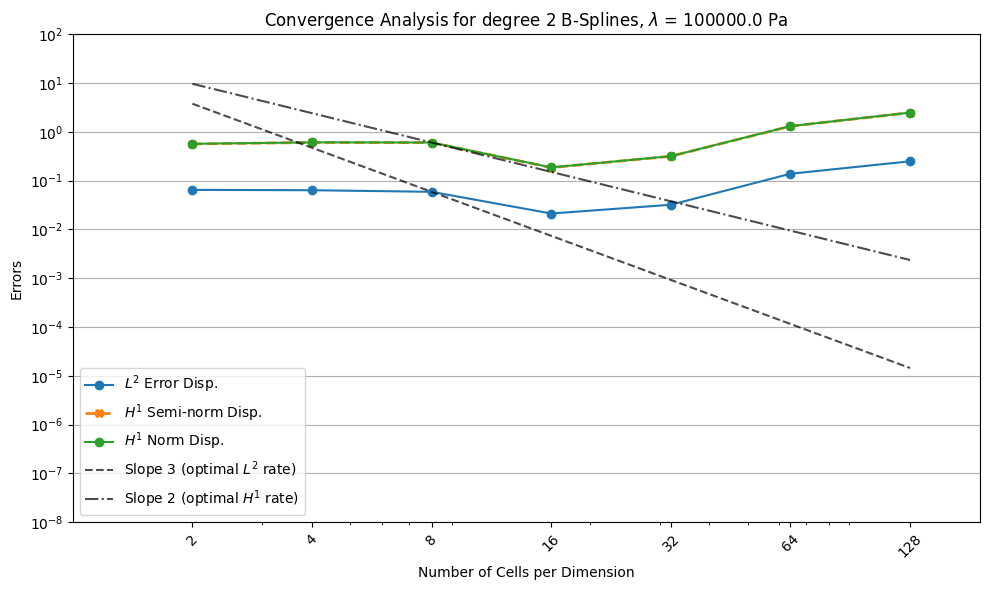
\includegraphics[width=\textwidth]{figures/figures_increasing_lambda_non_mixed/convergence_plot_degree_2_lambda=100000.0.png}
		\caption{$\lambda=100000$~Pa}
	\end{subfigure}
	\caption{Error plots between exact solution and numerical solution with degree 2 B-splines with increasing values of $\lambda$ with $\mu = 1$~Pa}
	\label{fig:error_kappa}
\end{figure}

As we can see in figure \ref{fig:error_kappa}, the convergence order is not respected anymore when $\lambda$ is too high compared to $\mu$. We can observe that when $\frac{\lambda}{\mu} = 10^4$, the error behaves like the error curves for rubber with degree 2 B-splines in figure \ref{fig:rubber_degree_2} $\displaystyle \left(\frac{\lambda_{\text{rubber}}}{\mu_{\text{rubber}}} \approx 500\right)$. Then, for values of $\lambda$ such that $\frac{\lambda}{\mu} \geq 10^4$, the error is not even decreasing anymore.

Two hypotheses can be made to explain this phenomenon: 
\begin{itemize}
	\item The estimates \eqref{eq:convergence_estimates} are not valid anymore, as $\lambda$ is too high compared to $\mu$.
	\item The bilinear form $a(.,.)$ is ill-conditioned, leading to numerical instability when $\lambda$ is "too high" compared to $\mu$.
\end{itemize}

One can try to increase the degree of B-splines to see if the convergence is reinforced as the power of $h$ in the estimates is higher. 

\begin{figure}[!h]
	\centering
	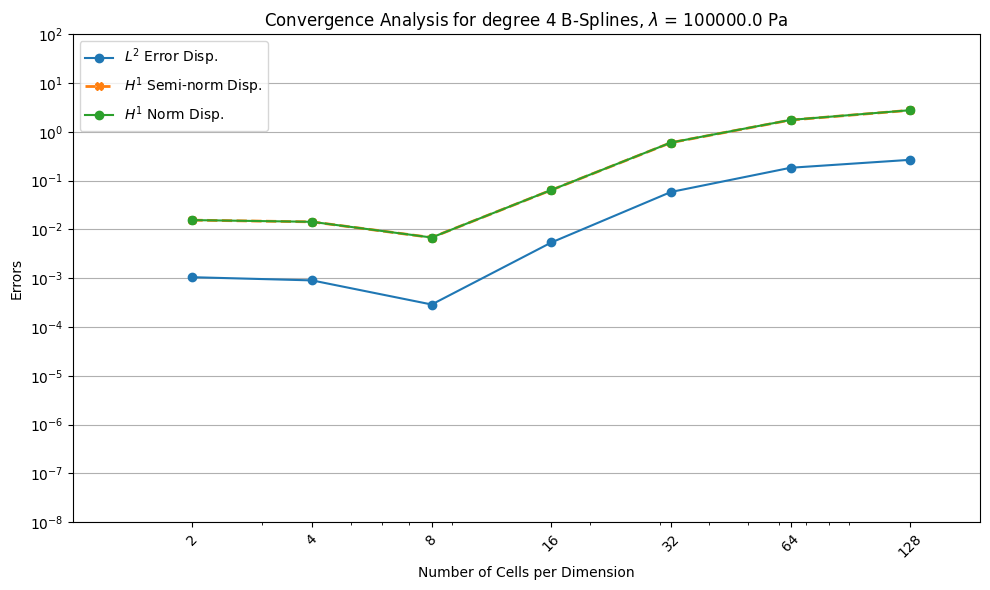
\includegraphics[width=0.8\textwidth]{figures/figures_increasing_lambda_non_mixed/convergence_plot_degree_4_lambda=100000.0.png}	
	\caption{Error plot between exact solution and numerical solution with degree 4 B-splines with $\lambda = 100000$~Pa and $\mu = 1$~Pa}
	\label{fig:error_kappa_degree_4}
\end{figure}

As we can see in figure \ref{fig:error_kappa_degree_4}, the convergence is not reinforced, the error is still not decreasing. Actually, this phenomenon is called \textbf{locking} and it is a well-known issue in FEM for incompressible materials. The locking occurs when the numerical solution is too stiff and does not converge to the real solution for high values of $\lambda$ compared to $\mu$.
One way to avoid this issue is to use a mixed formulation, where the pressure field is introduced as an additional variable. This will be presented in the next section.

\section{Mixed displacement-pressure formulation}
To introduce this formulation, let's consider again the strong formulation from \eqref{eq:strong_form}. Then, denote by $p$ the pressure field, defined by $\displaystyle p = - \lambda \div{\vec u}$. As we are seeking $\vec u \in \boldsymbol{H}^1(\Omega)$, $p$ is naturally living in $L^2(\Omega)$. Then Hooke's law can be rewritten as: $\boldsymbol{\sigma} (\vec u,p) = -p I_3 + 2\mu \boldsymbol{\varepsilon(\vec u)} \text{ in }  \Omega $ \\
So the strong formulation can be rewritten as: For a given $\vec f \in \boldsymbol L^2(\Omega)$, $\vec t_N \in \boldsymbol L^2(\partial \Omega_N)$, find $(\vec u, p) \in \boldsymbol H^1(\Omega)\times L^2(\Omega)$ such that: 

\begin{tcolorbox}
\begin{equation}
	\label{eq:strong_pressure_disp_form}
	\left\{
	\begin{aligned}
		& - \div \boldsymbol{\sigma} (\vec u,p) = \vec f & \text{ in } & \Omega \hspace{1cm} \text{(Equilibrium)}\\
		& \div{\vec u} + \frac{1}{\lambda} p = 0 & \text{ in } & \Omega \hspace{1cm} \text{(Pressure field definition)} \\
		& \vec u = \vec 0 & \text{ on } &\partial \Omega_D \\
		& \boldsymbol{\sigma} (\vec u) \cdot \vec n = \vec t_N & \text{ on }& \partial \Omega_N
	\end{aligned}
	\right.
\end{equation}
\end{tcolorbox}


Now, to derive the weak formulation, first we multiply the equilibrium equation by $v \in \boldsymbol H^1_{\vec 0,D}(\Omega)$ and integrate by parts on $\Omega$, then we multiply the pressure field equation by $q \in L^2(\Omega)$ and integrate over $\Omega$. Then we simply add both integrals. 
The weak formulation is then: 
\begin{tcolorbox}
\begin{equation}
	\label{eq:weak_pressure_displ_form}
	\left\{
	\begin{aligned}
		&\text{Find } (\vec u,p) \in \boldsymbol H^1_{\vec 0,D}(\Omega) \times L^2(\Omega) \text{ such that:}\\
		& \tilde{a}((\vec u,p),(\vec v,q)) = l(\vec v,q) \hspace{0.5cm} \forall (\vec v,q) \in \boldsymbol H^1_{\vec 0,D}(\Omega) \times L^2(\Omega)
	\end{aligned}
	\right.
\end{equation}
\end{tcolorbox}

With: 
\begin{equation*}
	\begin{aligned}
		& \tilde{a} : \left\{
		\begin{aligned}
			&\left( \boldsymbol H^1_{\vec 0,D}(\Omega) \times L^2(\Omega) \right)^2 \rightarrow \mtr \\
			&((\vec u,p),(\vec v,q))  \longmapsto \int_\Omega \left( 2\mu \boldsymbol{\varepsilon}(\vec u) : \boldsymbol{\varepsilon}(\vec v) - p (\div \vec v) + (\div \vec u)q + \frac{1}{\lambda} pq \right) \dif \Omega
		\end{aligned}
		\right. \\
		& l : 
		\left\{
		\begin{aligned}
			&\boldsymbol H^1_{\vec 0,D}(\Omega) \rightarrow \mtr \\
			&\vec v \longmapsto \int_\Omega \vec f \cdot \vec v \dif \Omega + \int_{\partial\Omega_N} \vec t_N \cdot \vec v \dif \Gamma
		\end{aligned}
		\right.
	\end{aligned}
\end{equation*}


\subsection{Well-posedness of the mixed displacement–pressure formulation}

Let
\[
V:=\boldsymbol H^1_{\vec 0,D}(\Omega),\qquad Q:=L^2(\Omega),\qquad X:=V\times Q,
\]
with the product norm
\[
\|(\vec u,p)\|_X^2 := \|\vec u\|_{\boldsymbol H^1(\Omega)}^2 + \|p\|_{L^2(\Omega)}^2.
\]

\noindent \textbf{Now, we can prove the well-posedness of \eqref{eq:weak_pressure_displ_form} for every finite }$\lambda>0, \mu>0$ \text{ and } $\Omega_D \neq \emptyset$.
\begin{itemize}
	\item $(X,\|\cdot\|_X)$ is a Hilbert space.
	\item $\tilde a(\cdot,\cdot)$ is a bilinear form on $X\times X$ and $l(\cdot)$ is linear on $X$.
	\item $l(\cdot)$ is continuous: for all $(\vec v,q)\in X$,
	\begin{equation*}
		\begin{aligned}
			|l(\vec v,q)|
			&\le |(\vec f,\vec v)_{\boldsymbol L^2(\Omega)}| + |(\vec t_N,\vec v)_{\boldsymbol L^2(\partial\Omega_N)}| \\
			&\le \Big(\|\vec f\|_{\boldsymbol L^2(\Omega)} + \norm{\gamma_0} \|\vec t_N\|_{\boldsymbol L^2(\partial\Omega_N)}\Big)\|\vec v\|_{H^1(\Omega)} \\
			|l(\vec v,q)| &\le C \big(\|\vec f\|_{\boldsymbol L^2(\Omega)} + \|\vec t_N\|_{\boldsymbol L^2(\partial\Omega_N)}\big)\|(\vec v,q)\|_X,
		\end{aligned}
	\end{equation*}
	where $\gamma_0$ is the trace operator and $C$ is a generic constant.
	\item $\tilde a(\cdot,\cdot)$ is continuous: for all $(\vec u,p),(\vec v,q)\in X$,
	\begin{equation*}
		\begin{aligned}
			|\tilde a((\vec u,p),(\vec v,q))|
			&\le 2\mu \|\boldsymbol{\varepsilon}(\vec u)\|_{L^2}\|\boldsymbol{\varepsilon}(\vec v)\|_{L^2}
				+ \|p\|_{L^2}\|\div \vec v\|_{L^2}
				+ \|\div \vec u\|_{L^2}\|q\|_{L^2}
				+ \tfrac{1}{\lambda}\|p\|_{L^2}\|q\|_{L^2} \\
			&\le 2 \mu \|\vec u\|_{\boldsymbol H^1}\|\vec v\|_{\boldsymbol H^1}
				+ 3 \|p\|_{L^2}\|\vec v\|_{\boldsymbol H^1}
				+ 3 \|\vec u\|_{\boldsymbol H^1}\|q\|_{L^2}
				+ \frac{1}{\lambda}\|p\|_{L^2}\|q\|_{L^2} \\
			&\le 2 \mu \| (\vec u,p)\|_X \|(\vec v,q)\|_X
				+ 3 \|(\vec u,p)\|_X \|(\vec v,q)\|_X
				+ 3 \|(\vec u,p)\|_X \|(\vec v,q)\|_X \\
				& + \frac{1}{\lambda}\|(\vec u,p)\|_X \|(\vec v,q)\|_X \\
			|\tilde a((\vec u,p),(\vec v,q))| &\le (2\mu + 6 + \frac{1}{\lambda})\|(\vec u,p)\|_X \|(\vec v,q)\|_X.
		\end{aligned}
	\end{equation*}
	using $\|\div \vec w\|_{L^2}\le 3 \|\vec w\|_{H^1}$, $\|p\|_{L^2} \le \|(\vec u,p)\|_X$ and $\|\vec u\|_{H^1} \le \|(\vec u,q)\|_X$.
	\item $\tilde a(\cdot,\cdot)$ is coercive on $X$: for all $(\vec u,p)\in X$,
	\begin{equation*}
		\tilde a((\vec u,p),(\vec u,p)) = 2\mu \|\boldsymbol{\varepsilon}(\vec u)\|_{L^2}^2 + \tfrac{1}{\lambda}\|p\|_{L^2}^2
		\ge 2\mu C_K^2 \|\vec u\|_{H^1}^2 + \tfrac{1}{\lambda}\|p\|_{L^2}^2
		\ge \alpha \|(\vec u,p)\|_X^2,
	\end{equation*}
	with $\alpha:=\min\{2\mu C_K^2,\,1/\lambda\}>0$ (for fixed finite $\lambda$).
\end{itemize}

Then, by the Lax–Milgram theorem, the mixed problem \eqref{eq:weak_pressure_displ_form} admits a unique solution $(\vec u,p)\in X$ and the stability estimate
\[
\|\vec u\|_{H^1(\Omega)}+\|p\|_{L^2(\Omega)} \le C\big(\|\vec f\|_{\boldsymbol L^2(\Omega)} + \|\vec t_N\|_{\boldsymbol L^2(\partial\Omega_N)}\big)
\]
holds with $C$ independent of $(\vec f,\vec t_N)$.

\noindent \textbf{Remark.} As $\lambda\to \infty$ (near-incompressible limit), the coercivity constant degenerates on the pressure component; the formulation approaches a saddle-point (Stokes-like) problem requiring an inf-sup (Ladyzhenskaya–Babuška–Brezzi) condition on the pair $(V,Q)$ to remain stable.

A way to ensure the inf-sup condition is to impose a zero mean value for the pressure field, i.e., $p\in L^2_0(\Omega)$, which is a common practice in numerical simulations of incompressible flows.

Then, the following inf-sup condition holds:
\[\inf_{q\in Q}\sup_{\vec v\in V}\frac{\tilde a((\vec v,q),(\vec u,p))}{\|\vec v\|_{H^1(\Omega)}\|q\|_{L^2(\Omega)}} \ge \beta > 0,\]
for some $\beta>0$ independent of $\lambda$ and $\mu$. This condition ensures the stability and the well-posedness of the mixed formulation with $V = H^1_0(\Omega)$ and $Q = L^2_0(\Omega)$ \cite{boffi_mixed_2008}.

If $\Omega_D = \emptyset$, the Dirichlet boundary condition is not imposed, and the problem becomes a pure Stokes problem. In this case, the uniqueness of the solution is guaranteed by the compatibility condition on the external loads, as discussed in Section \ref{sec:Pure displacement weak-formulation} modulo a rigid body motion.

\subsection{Isogeometric discretization and a priori error estimate}
Let $(V_h,Q_h)\subset V\times Q$ be the tensor–product B-spline spaces of (vector) degree $d$ (for the displacement) and (scalar) degree $d$ (for the pressure) with mesh size $h$, and assume that the discrete inf–sup condition holds with a constant $\beta>0$ independent of $h$, $\lambda$ and $\mu$ (locking–free setting) \cite{boffi_mixed_2008}. Then, for the exact solution $(\vec u_e,p_e)$ of \eqref{eq:weak_pressure_displ_form} and the discrete solution $(\vec u_h,p_h)\in V_h\times Q_h$, continuity plus coercivity on the kernel give the Céa-type bound
\[
\|\vec u_e-\vec u_h\|_{\boldsymbol H^1(\Omega)}+\|p_e-p_h\|_{L^2(\Omega)}
\;\le\; C\,\Big( \inf_{\vec w_h\in V_h}\|\vec u_e-\vec w_h\|_{\boldsymbol H^1(\Omega)} + \inf_{q_h\in Q_h}\|p_e-q_h\|_{L^2(\Omega)}\Big),
\]
with $C > 0$, and \textit{a priori} $C \propto \frac{2\mu + 6 + 1/\lambda}{\min(2\mu C_K^2,1 / \lambda)}$. For $(\vec u,p)$ sufficiently smooth, namely $\vec u\in \boldsymbol H^{d+1}(\Omega)$ and $p\in H^{d}(\Omega)$, spline approximation estimates yield
\[
\|\vec u_e-\vec u_h\|_{\boldsymbol H^1(\Omega)}+\|p_e-p_h\|_{L^2(\Omega)} \;\le\; C h^{d}\Big(\|\vec u_e\|_{\boldsymbol H^{d+1}(\Omega)}+\|p_e\|_{H^{d}(\Omega)}\Big),
\]
Then, while $2 \mu C_K^2 > \frac{1}{\lambda}$, the coercivity constant $\alpha$ is bounded away from zero, and the estimate holds uniformly in $\lambda$ and $\mu$. But when $\lambda \rightarrow \infty$, the coercivity constant $\alpha$ tends to zero, leading to a loss of stability in the numerical method. Now we can look at the convergence estimates for the mixed displacement-pressure formulation to see if this formulation can solve for higher values of $\frac{\lambda}{\mu}$ than the pure-displacement formulation.


\subsection{Example of simulation using \texttt{PSYDAC}}
In this section, we will present the results of a simulation using the mixed displacement-pressure formulation with B-splines. 

For the manufactured solution, we will use the same one as in Section \ref{subsec:Dirichlet Homogeneous Boundary conditions on}. For reference, the exact solution is given by:
$$
\vec u_e(x,y,z)=
\begin{pmatrix}
0\\[2pt]
0\\[2pt]
\sin(\pi x)\sin(\pi y)\sin(\pi z)
\end{pmatrix},\qquad
p_e(x,y,z)= -\lambda\,\div \vec u_e = -\lambda \pi \sin(\pi x)\sin(\pi y)\cos(\pi z).
$$

$$
\vec f = -\div \boldsymbol\sigma(\vec u_e,p_e)=
\begin{pmatrix}
-\pi^{2}(\lambda+\mu)\cos(\pi x)\sin(\pi y)\cos(\pi z)\\[4pt]
-\pi^{2}(\lambda+\mu)\sin(\pi x)\cos(\pi y)\cos(\pi z)\\[4pt]
\pi^{2}(\lambda+4\mu)\sin(\pi x)\sin(\pi y)\sin(\pi z)
\end{pmatrix}.
$$
And the boundary conditions are: 
\begin{align*}
\vec u_e|_{\partial\Omega} &= 0,\\
p_e|_{\partial\Omega} &= \begin{cases}
-\lambda \pi \sin(\pi x) \sin(\pi y) & \text{if } z = 0 \\
\lambda \pi \sin(\pi x) \sin(\pi y) & \text{if } z = 1
\end{cases}
\end{align*}

Since the exact solution now depends on $\lambda$, we will look at the relative error between exact and numerical solutions for different values of $\lambda$. (This wasn't necessary before as the exact solution was independent of $\lambda$, so the norm of the exact solution was the same for all values of $\lambda$).
To do so, we can look at the relative error between exact and numerical solution, defined by: 
$$
E_{rel} = \frac{\|\vec u_e - \vec u_h\|_{H^1} + \|p_e - p_h\|_{L^2}}{\|\vec u_e\|_{H^1} + \|p_e\|_{L^2}}.
$$
and its variation across the number of cells for different values of $\lambda$.

\begin{figure}[!h]
	\centering
	\begin{subfigure}[b]{0.49\textwidth}
		\centering
		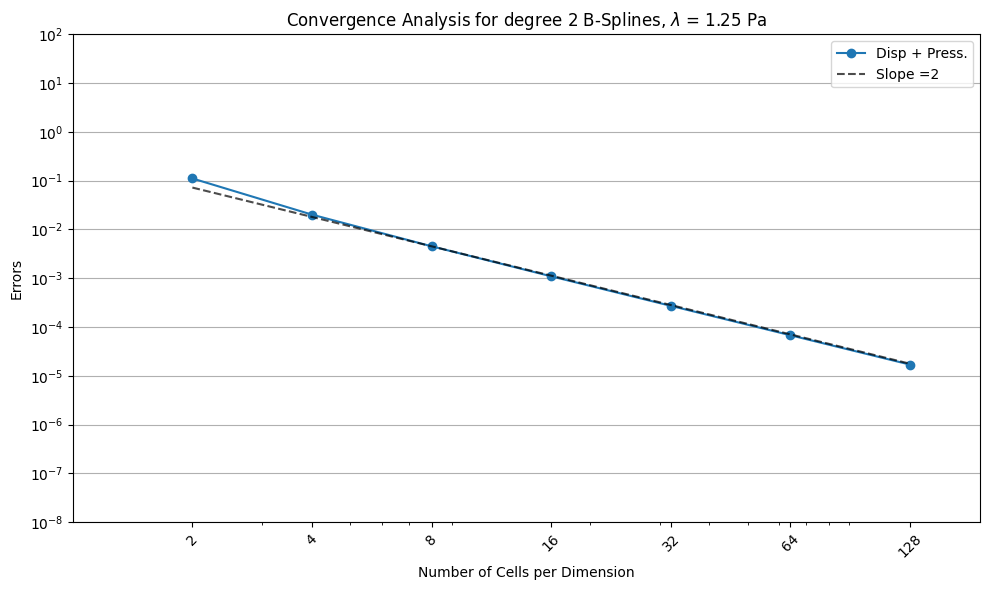
\includegraphics[width=\textwidth]{figures/figures_mixed_DH/sum_convergence_plot_degree_2_lambda=1.25.png}
		\caption{$E_{rel}(n_{\text{cells}})$ with $\lambda = 1.25$~Pa and $\frac{\lambda}{\mu} = 1.25$}
		\label{fig:convergencedegree2mixeddirichlethomogeneouslambda1.25}
	\end{subfigure}
	\begin{subfigure}[b]{0.49\textwidth}
		\centering
		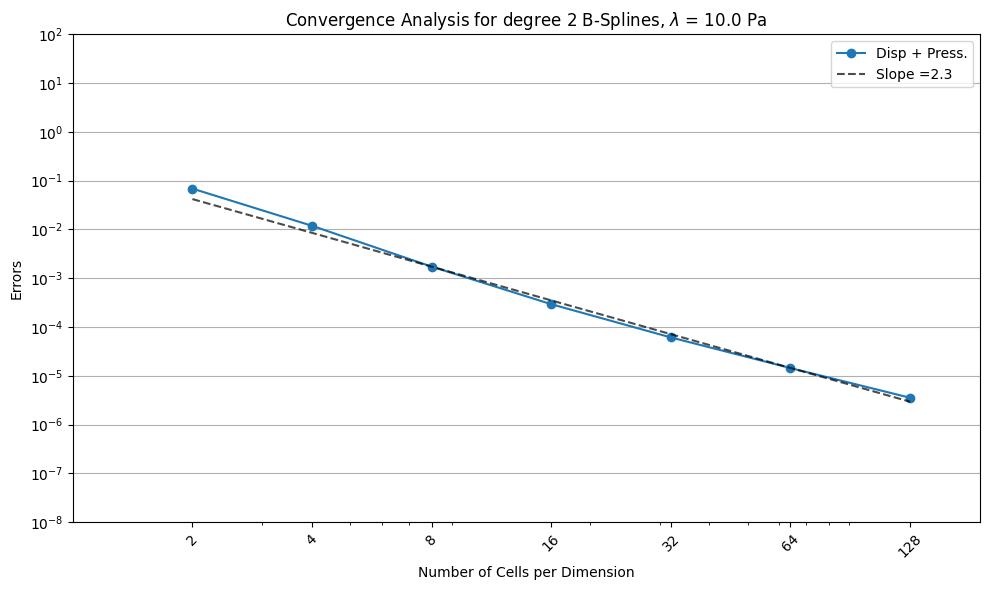
\includegraphics[width=\textwidth]{figures/figures_mixed_DH/sum_convergence_plot_degree_2_lambda=10.0.png}
		\caption{$E_{rel}(n_{\text{cells}})$ with $\lambda = 10$~Pa and $\frac{\lambda}{\mu} = 10$}
		\label{fig:convergencedegree2mixeddirichlethomogeneouslambda10}
	\end{subfigure}
	\begin{subfigure}[b]{0.49\textwidth}
		\centering
		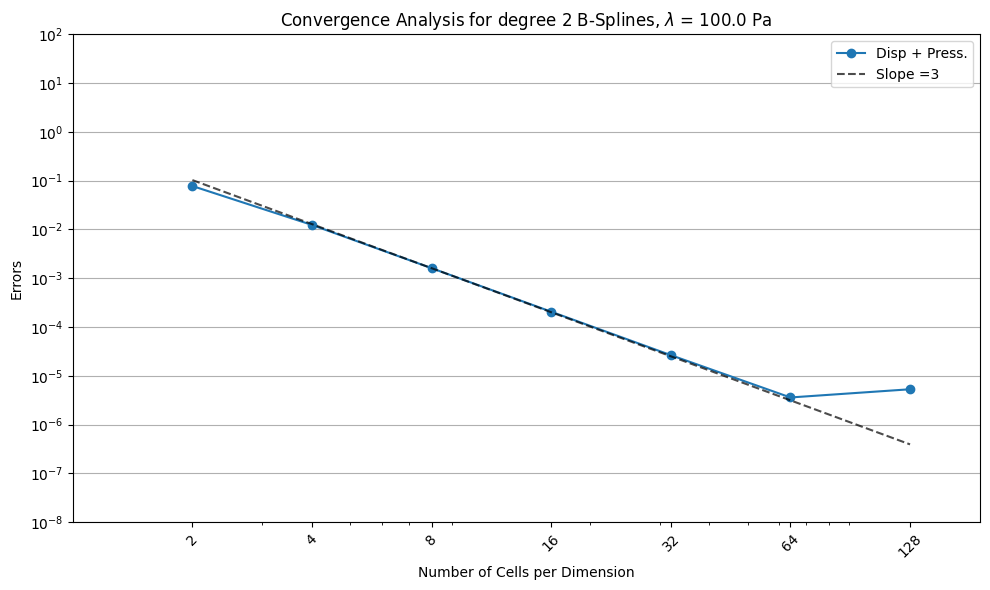
\includegraphics[width=\textwidth]{figures/figures_mixed_DH/sum_convergence_plot_degree_2_lambda=100.0.png}
		\caption{$E_{rel}(n_{\text{cells}})$ with $\lambda = 100$~Pa and $\frac{\lambda}{\mu} = 100$}
		\label{fig:convergencedegree2mixeddirichlethomogeneouslambda100}
	\end{subfigure}
	\begin{subfigure}[b]{0.49\textwidth}
		\centering
		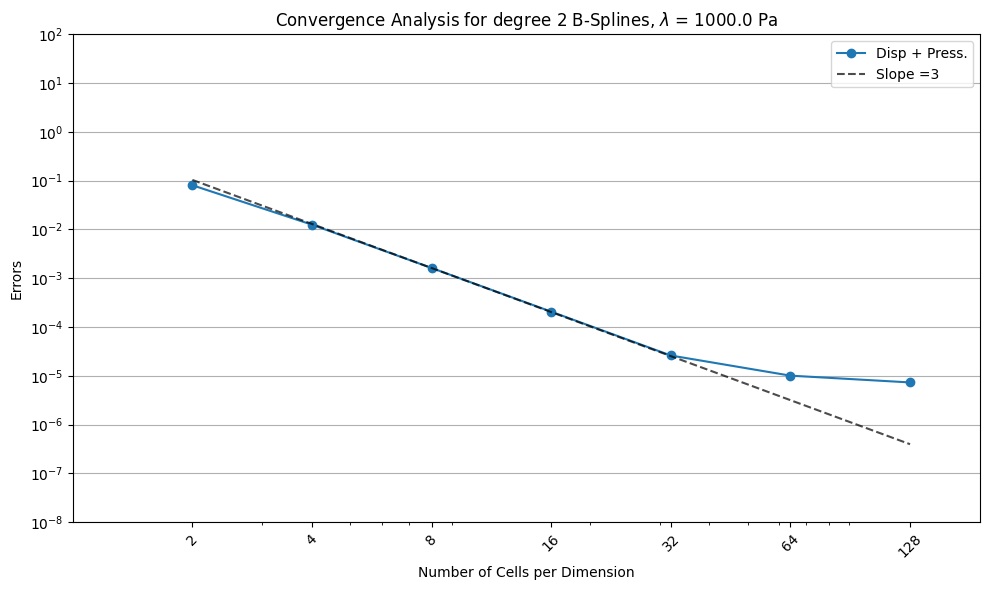
\includegraphics[width=\textwidth]{figures/figures_mixed_DH/sum_convergence_plot_degree_2_lambda=1000.0.png}
		\caption{$E_{rel}(n_{\text{cells}})$ with $\lambda = 10^3$~Pa and $\frac{\lambda}{\mu} = 1000$}
		\label{fig:convergencedegree2mixeddirichlethomogeneouslambda1000}
	\end{subfigure}
\end{figure}
\begin{figure}[!h] \ContinuedFloat
	\centering
	\begin{subfigure}[b]{0.49\textwidth}
		\centering
		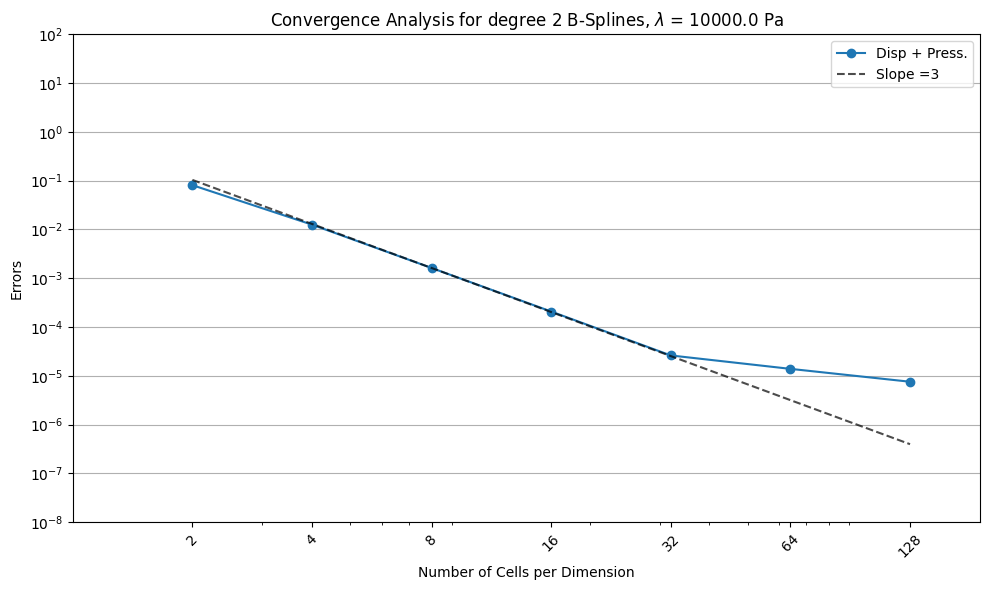
\includegraphics[width=\textwidth]{figures/figures_mixed_DH/sum_convergence_plot_degree_2_lambda=10000.0.png}
		\caption{$E_{rel}(n_{\text{cells}})$ with $\lambda = 10^4$~Pa and $\frac{\lambda}{\mu} = 10000$}
		\label{fig:convergencedegree2mixeddirichlethomogeneouslambda10000}
	\end{subfigure}
	\begin{subfigure}[b]{0.49\textwidth}
		\centering
		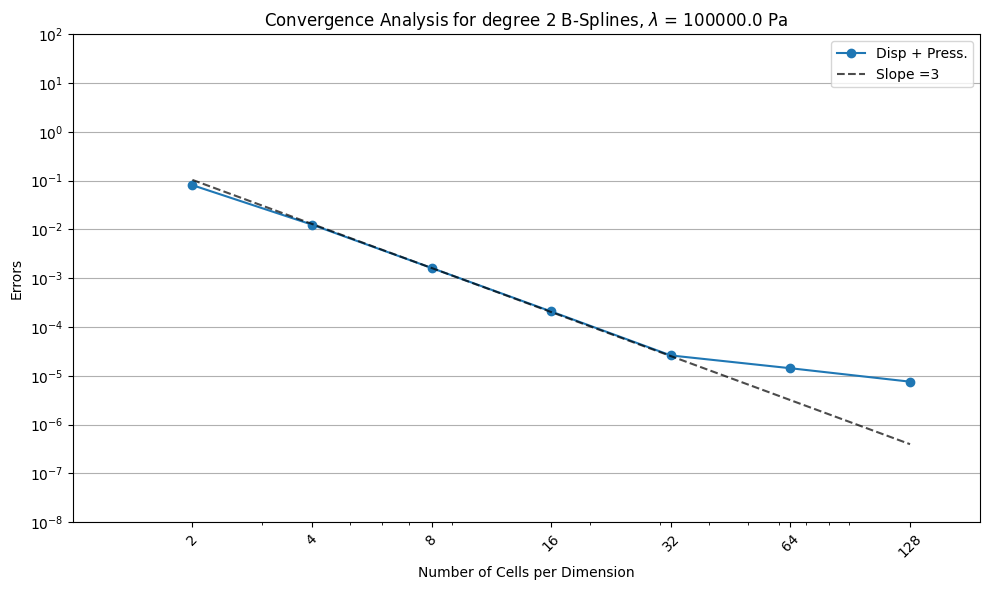
\includegraphics[width=\textwidth]{figures/figures_mixed_DH/sum_convergence_plot_degree_2_lambda=100000.0.png}
		\caption{$E_{rel}(n_{\text{cells}})$ with $\lambda = 10^5$~Pa and $\frac{\lambda}{\mu} = 100000$}
		\label{fig:convergencedegree2mixeddirichlethomogeneouslambda100000}
	\end{subfigure}
	\begin{subfigure}[b]{0.49\textwidth}
		\centering
		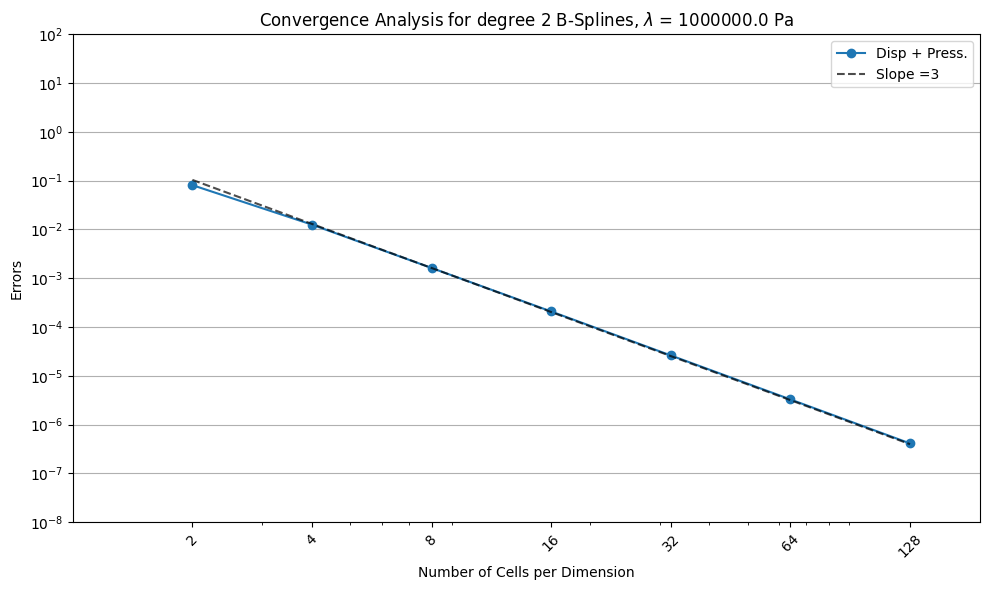
\includegraphics[width=\textwidth]{figures/figures_mixed_DH/sum_convergence_plot_degree_2_lambda=1000000.0.png}
		\caption{$E_{rel}(n_{\text{cells}})$ with $\lambda = 10^6$~Pa and $\frac{\lambda}{\mu} = 1000000$}
		\label{fig:convergencedegree2mixeddirichlethomogeneouslambda1000000}
	\end{subfigure}
		\begin{subfigure}[b]{0.49\textwidth}
		\centering
		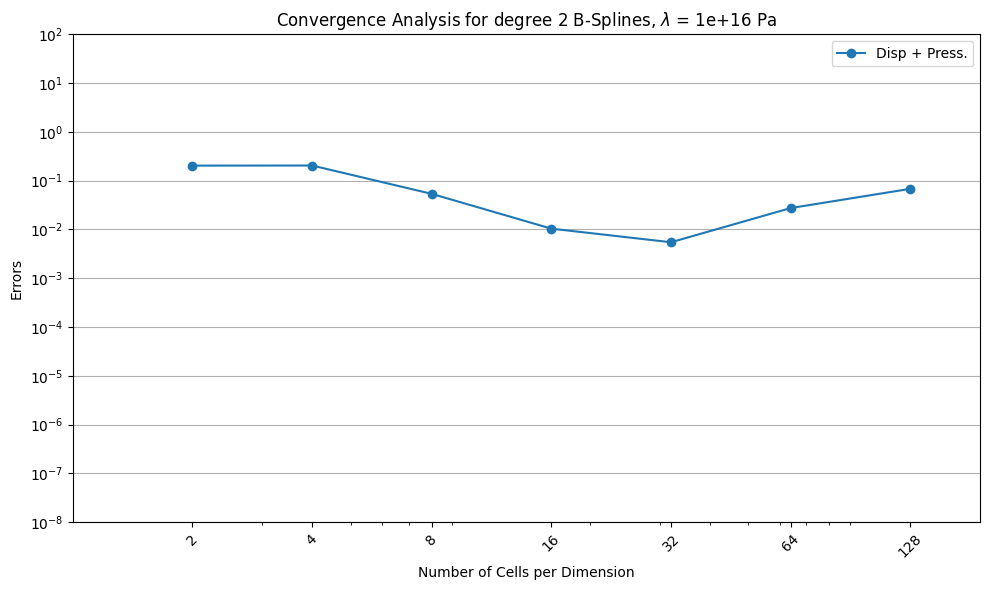
\includegraphics[width=\textwidth]{figures/figures_mixed_DH/sum_convergence_plot_degree_2_lambda=1e+16.png}
		\caption{$E_{rel}(n_{\text{cells}})$ with $\lambda = 10^{16}$~Pa and $\frac{\lambda}{\mu} = 10^{16}$}
		\label{fig:convergencedegree2mixeddirichlethomogeneouslambda1e16}
	\end{subfigure}
	\caption{Relative error between exact and numerical solution with degree 2 B-splines for different values of $\lambda$}
	\label{fig:convergencedegree2mixeddirichlethomogeneous}
\end{figure}


The convergence analysis presented in Figure \ref{fig:convergencedegree2mixeddirichlethomogeneous} reveals several important characteristics of the mixed displacement-pressure formulation across different Lamé parameter values. This comprehensive study examines the behavior of the numerical scheme for values of $\lambda$ ranging from $1.25$~Pa to $10^{16}$~Pa, corresponding to materials from highly compressible to nearly incompressible regimes.

We can observe that from $\frac{\lambda}{\mu} = 100$, the convergence behavior is robust and follows a $-3$ slope. This indicates that the mixed formulation maintains optimal convergence properties even as the material approaches incompressibility. The observed slope is higher than expected. This could be due to the fact that as $\lambda$ increases, the pressure variable becomes more dominant in the formulation and influences the overall convergence behavior. This is only an intuition and an interpretation of the error plots, and further analysis would be needed to confirm this hypothesis. That has not been done yet.
The plateau phenomenon is observed again when the error reaches a certain threshold and no longer decreases significantly with mesh refinement.

However, when $\frac{\lambda}{\mu} \gg 1$, so here $\frac{\lambda}{\mu} = 10^{16}$, the same phenomenon as in the pure displacement formulation occurs, where the error does not decrease anymore. This is likely due to the fact that the pressure variable is not able to compensate for the locking phenomenon that occurs when $\lambda$ is too high compared to $\mu$. We can suppose that the coercivity constant $\alpha$ has reached its limit and now $\alpha = \frac{1}{\lambda}$.

When we look at the continuity and coercivity constants of the bilinear form $a$, one can also think that the more $\mu$ becomes higher, the more this loss of coercivity will appear faster when $\lambda \rightarrow \infty$.

For example, if we consider steel's Lamé parameters, which are typically around $\lambda = 120$~GPa and $\mu = 80$~GPa, we find that $\frac{\lambda}{\mu} = 1.5$. As we can see in the following error plot, the locking phenomenon appears.

\begin{figure}[!h]
	\centering
	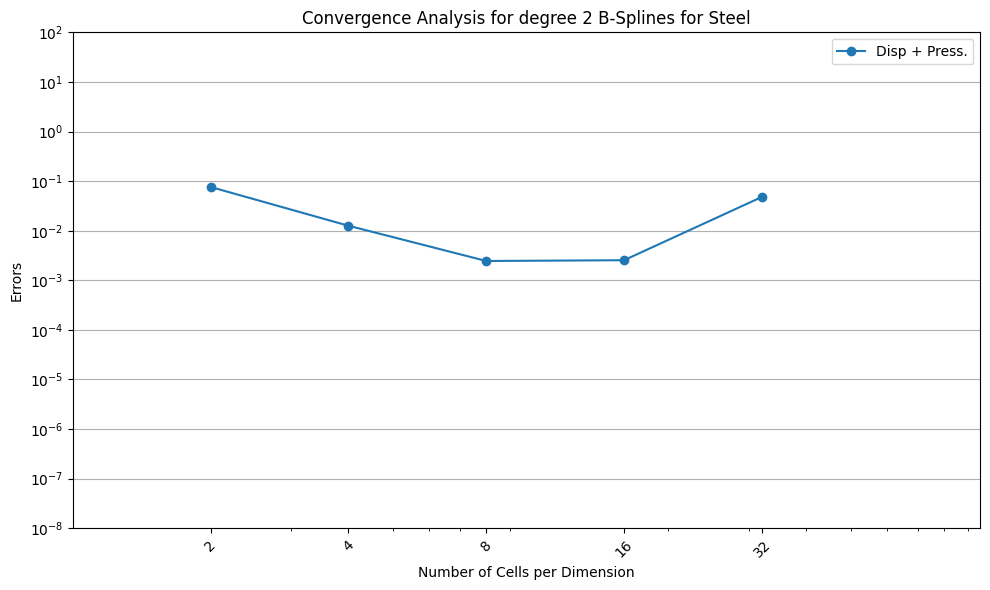
\includegraphics[width=0.8\textwidth]{figures/figures_mixed_DH/sum_convergence_plot_degree_2_lambda=120000000000.0.png}
	\caption{Relative error between exact and numerical solution with degree 2 B-splines for steel's Lamé parameters}
	\label{fig:convergencedegree2mixeddirichlethomogeneoussteel}
\end{figure}

The same behavior is actually observed for rubber and concrete, even if the ratio $\frac{\lambda}{\mu}$ is not as high as in \ref{fig:convergencedegree2mixeddirichlethomogeneouslambda1e16}. This is due to the fact that with the mixed formulation, when $\mu$ increases, the coercivity constant $\alpha$ becomes smaller faster when $\lambda$ increases.

\section{Conclusion}

This chapter presented a study of linear elasticity formulations implemented with \texttt{PSYDAC}, demonstrating the library's capability to handle solid mechanics problems beyond its original plasma physics applications. Two distinct formulations were investigated: the pure displacement formulation and the mixed displacement-pressure formulation, each offering unique advantages for different material regimes.

The pure displacement formulation proved effective for materials with moderate Lamé parameter ratios, achieving optimal convergence rates as predicted by theoretical estimates. However, the study revealed significant limitations when dealing with nearly incompressible materials, where the ratio $\frac{\lambda}{\mu}$ becomes large. The locking phenomenon observed for values of $\frac{\lambda}{\mu} \geq 10^4$ demonstrates the practical limitations of this approach for such materials, with convergence rates deteriorating significantly or even failing entirely.

The mixed displacement-pressure formulation successfully addressed many of the incompressibility issues inherent in the pure displacement approach. By introducing pressure as an additional variable, this formulation maintained robust convergence behavior for much higher values of $\frac{\lambda}{\mu}$, effectively extending the applicable range to materials approaching the incompressible limit. 

Both formulations were thoroughly validated using the method of manufactured solutions across various material parameters, mesh refinements, and B-spline degrees. The convergence studies confirmed the expected optimal rates, with the occasional plateau effects attributed to matrix ill-conditioning at very fine mesh resolutions and a limited number of solver iterations. The successful implementation on the Raven supercomputer demonstrated \texttt{PSYDAC}'s scalability and performance capabilities for large-scale solid mechanics simulations.

The comprehensive comparison between these formulations provides valuable insights for practitioners choosing appropriate numerical methods based on material properties. For standard engineering materials like steel and concrete, where $\frac{\lambda}{\mu}$ remains moderate, the pure displacement formulation offers computational efficiency and straightforward implementation. For applications involving nearly incompressible materials or when robustness across a wide range of material parameters is required, the mixed formulation provides superior stability and accuracy.

This work has contributed to expanding \texttt{PSYDAC}'s application domain while maintaining its high-order accuracy and geometric flexibility. The implementations developed during this study are available as interactive Jupyter notebooks demonstrating both formulations, accessible through the IGA-Python repository: \href{https://github.com/pyccel/IGA-Python/pull/21}{https://github.com/pyccel/IGA-Python/pull/21}. These resources provide practical examples and can serve as starting points for further developments in computational solid mechanics using isogeometric analysis.


\chapter{Thermoelasticity}
\section{Introduction}
This chapter is dedicated to the study of the thermoelasticity problem, which is a coupled problem between the mechanical and thermal fields. The aim is to solve the coupled system of equations that governs the behavior of a thermoelastic material under thermal and mechanical loads. This work was initiated to solve a problem presented during the IPP Programme Days 2025 by Prof. Dr. Rudolf Neu. The goal is to understand the deformation of a medium under the influence of thermal loads and mechanical forces. The medium is a composite material, composed of copper and tungsten. The geometry is presented in the following figure.
\begin{figure}[!h]
	\centering
	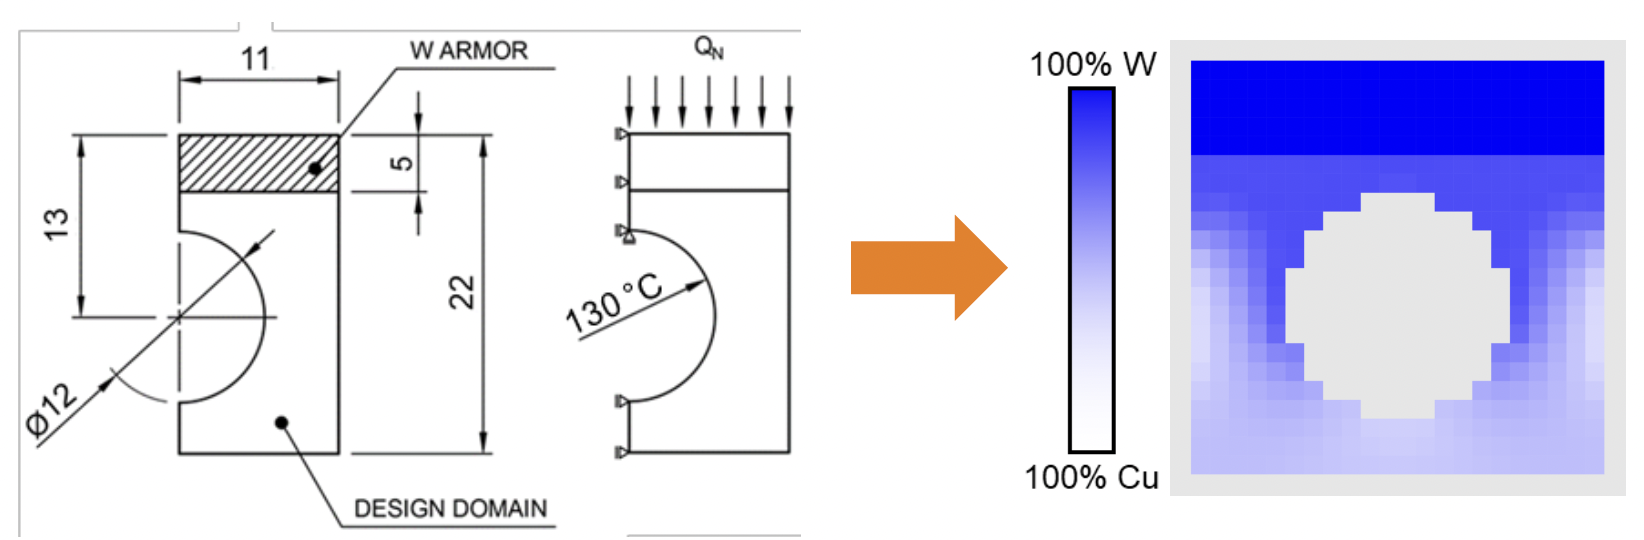
\includegraphics[width=0.7\textwidth]{figures/geometry_thermoelasticity.png}
	\caption{Geometry of the thermoelasticity problem from the IPP Programme Days 2025}
	\label{fig:geometry_thermoelasticity}
\end{figure}

\section{Simplified problem - Physical model and equations}

Before solving this problem, I want to simplify it a bit by considering a slightly different geometry, which is a square without the hole in the middle. The goal is to understand the behavior of the medium under thermal and mechanical loads, to see how the deformation of the medium is affected by the thermal loads and to see if PSYDAC can effectively solve this simplified problem. The geometry of the simplified problem is presented in figure \ref{fig:geometry_thermoelasticity_simplified}.

\subsection{Problem setup and parameters}
\label{subsec:problem_setup_parameters}
The problem can be parameterized as follows with other boundary conditions and parameters:
\begin{itemize}
	\item The domain $\Omega$ is a square of size $22$: $\Omega = [0,22]^2$.
	\item $\partial \Omega_{\text{heat}} = \{(x,y) \in \partial \Omega \,|\, x = 0 \text{ and } x = 22 \}$ is the left and right edges of the square, where heat $Q$ is applied. $\partial \Omega_{\text{temp}} = \{(x,y) \in \partial \Omega \,|\, y = 0 \text{ and } y = 22\}$ is the top and bottom edges of the square, where the temperature is fixed to $T_0$.
	\item $\partial \Omega_{D} = \{(x,y) \in \partial \Omega \,|\, x = 0 \text{ and } x = 22 \}$ are the left and right edges of the square, where the Dirichlet boundary conditions are applied and the displacement is fixed. $\partial \Omega_{N} = \{(x,y) \in \partial \Omega \,|\, y = 0 \text{ and } y = 22\}$ are the top and bottom edges of the square, where the Neumann boundary conditions are applied and the traction is fixed.
	\item For $y \in (0, 17)$, the material is composite and properties are given by an affine interpolation between copper and tungsten properties.
	For $y \in (17, 22)$, the material is pure tungsten. 
	For example, $\lambda$ is defined as:
	\[\lambda(y) = \begin{cases}
		\lambda_{\text{Cu}} + \frac{y}{17}(\lambda_{\text{W}} - \lambda_{\text{Cu}}) & \text{if } y \in (0, 17) \\
		\lambda_{\text{W}} & \text{if } y \in (17, 22)
	\end{cases}\]
	\item The material properties are given by: 
	\begin{table}[h!]
	\centering
	\begin{tabular}{lcc}
	\hline
	\textbf{Property} & \textbf{Cu} & \textbf{W} \\
	\hline
	Lamé's first constant $\lambda$ [Pa] & $1.1\times 10^{11}$ & $2.5\times 10^{11}$ \\
	Shear modulus $\mu$ [Pa]             & $4.1\times 10^{10}$ & $1.6\times 10^{11}$ \\
	Thermal expansion $\alpha$ [1/K]     & $1.7\times 10^{-5}$ & $4.5\times 10^{-6}$ \\
	Thermal conductivity $\kappa$ [W/(m$\cdot$K)] & $401$ & $174$ \\
	\hline
	\end{tabular}
	\caption{Material properties of Copper (Cu) and Tungsten (W).}
	\end{table}
\end{itemize}

\begin{figure}[!h]
	\centering
	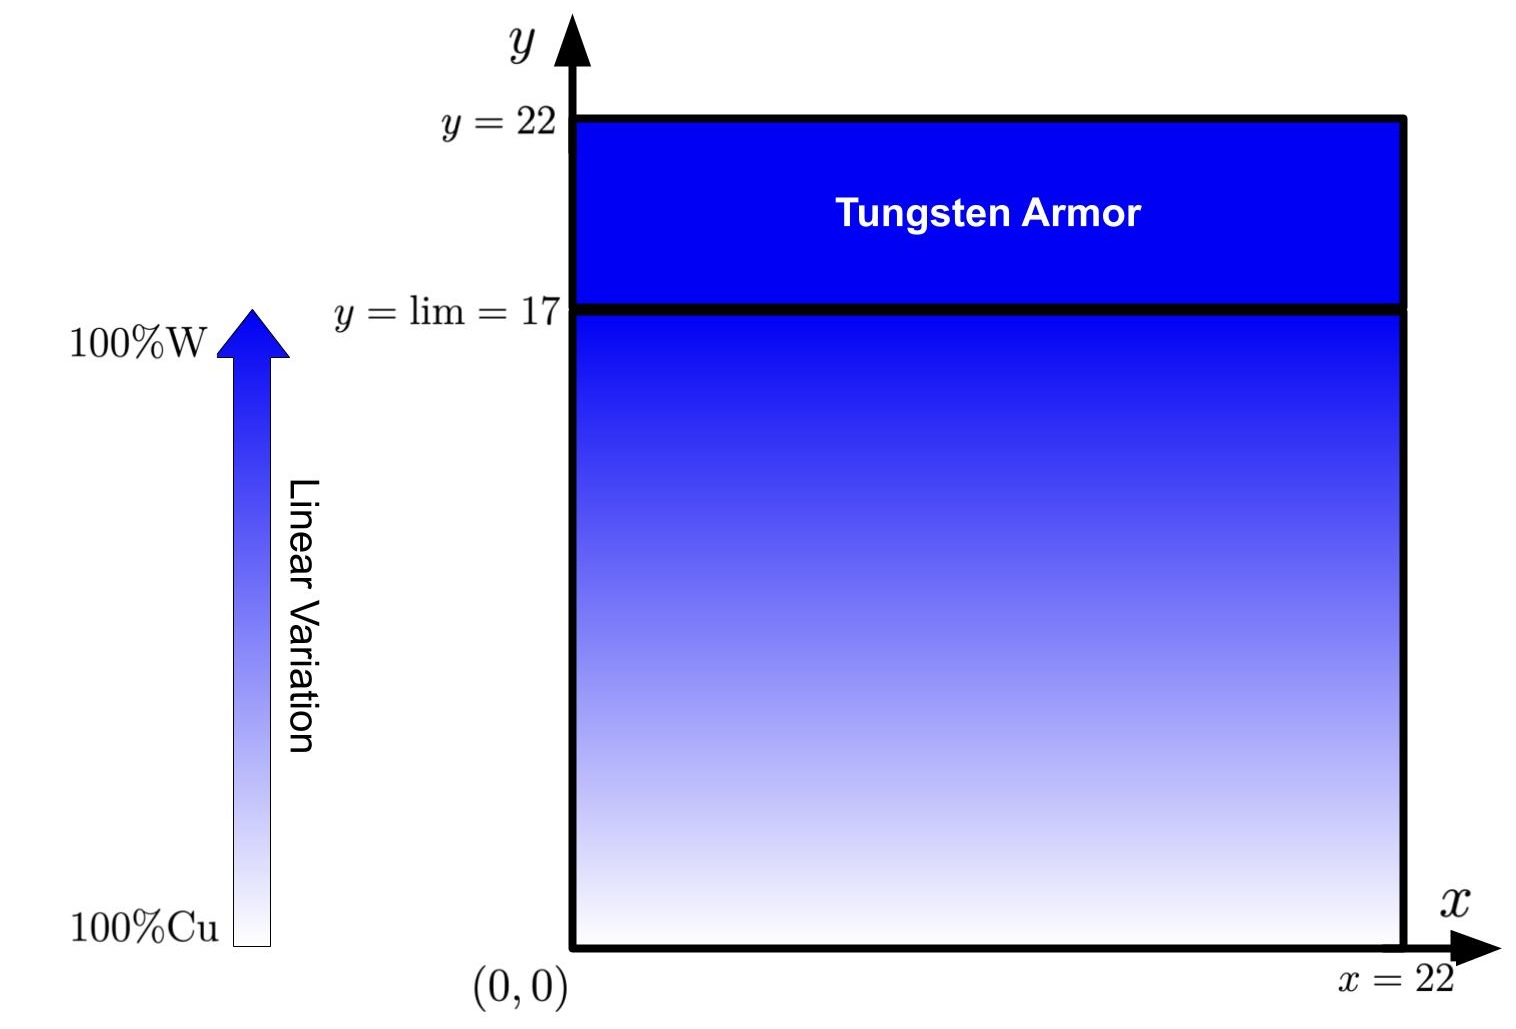
\includegraphics[width=0.6\textwidth]{figures/geometry_thermoelasticity_simplified.jpg}
	\caption{Geometry of the simplified thermoelasticity problem}
	\label{fig:geometry_thermoelasticity_simplified}
\end{figure}

\subsection{Strong Formulation}
The presentation of the strong formulation of the thermoelasticity problem is based on the principles of continuum mechanics and thermodynamics taken from \cite{MeyerSpringer2015} and \cite{Persson2016}. The thermoelasticity problem is a coupled problem between the mechanical and thermal fields. The equations that govern the behavior of a thermoelastic material are given by the coupling of the heat equation and the elasticity equation.

The full time-dependent thermoelasticity equations are:
\begin{equation}
	\left\{
	\begin{aligned}
		\rho(y) c_p(y) \frac{\partial T}{\partial t} + \div (\kappa(y) \grad T) &= Q - (3\lambda(y) + 2\mu(y))\alpha(y) T_0 \frac{\partial}{\partial t} (\div \vec u) \\
		\rho(y) \frac{\partial^2 \vec u}{\partial t^2} - \div \boldsymbol{\sigma}(\vec u) &= \vec f  \\
		\boldsymbol{\sigma}(\vec u) &= \lambda(y) (\div \vec u) I_3 + 2\mu(y) \boldsymbol{\varepsilon}(\vec u) - (3\lambda(y) + 2\mu(y)) \alpha(y) T I_3 
	\end{aligned}
	\right.
\end{equation}

where $\rho(y)$ is the density, $c_p(y)$ is the specific heat capacity at constant pressure, $T$ is the temperature, $\kappa(y)$ is the thermal conductivity, $Q$ is the heat source, $\vec u$ is the displacement field, $\vec f$ is the body force, $\boldsymbol{\sigma}$ is the stress tensor, $\lambda(y)$ and $\mu(y)$ are the Lamé coefficients, $\boldsymbol{\varepsilon}$ is the strain tensor, $\alpha(y)$ is the thermal expansion coefficient and $T_0$ is the reference temperature.

For this study, we will consider the stationary case, where the time derivatives are zero ($\frac{\partial T}{\partial t} = 0$ and $\frac{\partial^2 \vec u}{\partial t^2} = 0$). This simplifies the system to:
\begin{equation*}
	\left\{
	\begin{aligned}
		- \div (\kappa(y) \grad T) &= Q \\
		- \div \boldsymbol{\sigma}(\vec u) &= \vec f \\
		\boldsymbol{\sigma}(\vec u) &= \lambda(y) (\div \vec u) I_3 + 2\mu(y) \boldsymbol{\varepsilon}(\vec u) - (3\lambda(y) + 2\mu(y)) \alpha(y) T I_3 
	\end{aligned}
	\right.
\end{equation*}
These stationary equations represent the equilibrium state of the thermoelastic material under constant thermal and mechanical loads.

To complete the problem formulation, we must specify the boundary conditions. Based on the problem description, we have the following conditions on the boundary $\partial\Omega$:

For the thermal problem:
\begin{align}
	T &= T_0 \quad &&\text{on } \partial\Omega_{\text{temp}} \label{eq:bc_temp_dirichlet_thermoelastic} \\
	- \kappa \grad T \cdot \vec n &= q_S \quad &&\text{on } \partial\Omega_{\text{heat}} \label{eq:bc_temp_neumann_thermoelastic}
\end{align}
where $T_0$ is the reference temperature and $q_S$ is the applied heat flux on the boundary.

For the mechanical problem:
\begin{align}
	\vec u &= \vec u_D \quad &&\text{on } \partial\Omega_D \label{eq:bc_disp_dirichlet_thermoelastic} \\
	\boldsymbol{\sigma}(\vec u) \cdot \vec n &= \vec t_N \quad &&\text{on } \partial\Omega_N \label{eq:bc_disp_neumann_thermoelastic}
\end{align}
where $\vec u_D$ is the prescribed displacement and $\vec t_N$ is the prescribed traction. 
To prove the well-posedness of the problem, we will limit the analysis to $T_0 = 0$ and $\vec u_D = \vec 0$, otherwise the problem can be rewritten with homogeneous boundary conditions with a change of variables.
 
For a given $Q \in L^2(\Omega)$, $q_S \in L^2(\partial \Omega_{\text{heat}})$, $\vec f \in \boldsymbol L^2(\Omega)$, $\vec t_N \in \boldsymbol L^2(\partial \Omega_N)$, the entire strong problem is:
\begin{tcolorbox}
Find $(T,\vec u) \in H^1(\Omega) \times \boldsymbol H^1_{\vec 0,D}(\Omega)$ such that:
\begin{align}
	- \div (\kappa(y) \grad T) &= Q && \text{in } \Omega \\
	- \div \boldsymbol{\sigma}(\vec u) &= \vec f && \text{in } \Omega \\
	\boldsymbol{\sigma}(\vec u) &= \lambda(y) (\div \vec u) I_3 + 2\mu(y) \boldsymbol{\varepsilon}(\vec u) - (3\lambda(y) + 2\mu(y)) \alpha(y) T I_3 && \text{in } \Omega \\
	\vec u &= \vec 0 && \text{on } \partial\Omega_D \\
	\boldsymbol{\sigma}(\vec u) \cdot \vec n &= \vec t_N && \text{on } \partial\Omega_N \\
	T &= 0 && \text{on } \partial\Omega_{\text{temp}} \\
	-\kappa(y) \grad T \cdot \vec n &= q_S && \text{on } \partial\Omega_{\text{heat}}
\end{align}
\end{tcolorbox}

This problem can be seen as a coupled thermo-mechanical problem, where the temperature field $T$ affects the mechanical behavior of the material through the thermal expansion term in the stress tensor $\boldsymbol{\sigma}(\vec u)$, but the mechanical displacement $\vec u$ does not directly affect the temperature field $T$. So, to solve this problem, one can first solve the thermal problem to obtain the temperature field $T$, and then use this temperature field to solve the mechanical problem for the displacement $\vec u$ with a modified source term that includes the thermal expansion effects. As $\displaystyle \forall y \in [0,22], \frac{\lambda(y)}{\mu(y)} \leq 50$, according to results from Subsection \ref{sec:mixed_BC}, we can use the pure displacement formulation to solve the mechanical problem.

\subsection{Weak Formulation}

The corresponding weak formulation is obtained by multiplying the PDEs by suitable test functions, integrating over the domain $\Omega$, and applying integration by parts.

Let the solution space for temperature be $H^1_{0,\text{temp}} = \{ \phi \in H^1(\Omega) \mid \phi = 0 \text{ on } \partial\Omega_{\text{temp}} \}$ and for displacement be $\boldsymbol{H}^1_{\vec 0,D}(\Omega)$. The weak problem is:
\begin{tcolorbox}
Find $(T, \vec u) \in H^1_{0,\text{temp}} \times \boldsymbol{H}^1_{\vec 0,D}(\Omega)$ such that for all test functions $(\theta, \vec v) \in H^1_{0,\text{temp}} \times \boldsymbol{H}^1_{\vec 0,D}(\Omega)$:
\begin{equation}
	\left\{
	\begin{aligned}
		b(T, \theta) &= l_T(\theta) \\
		a(\vec u, \vec v) &= l_U(\vec v)
	\end{aligned}
	\right.
\end{equation}
\label{eq:weak-thermoelasticity}
\end{tcolorbox}
With 
\begin{equation*}
	\begin{aligned}
	& b : \left\{
		\begin{aligned}
			& H^1_{0,\text{temp}} \times H^1_{0,\text{temp}} \longrightarrow \mtr \\
			& (T, \theta) \mapsto \int_{\Omega} \kappa(y) \grad T \cdot \grad \theta \, d\Omega 
		\end{aligned}
	\right. \\
	& l_T : \left\{
		\begin{aligned}
			& H^1_{0,\text{temp}} \longrightarrow \mtr \\
			& \theta \mapsto\int_{\Omega} Q \theta \, d\Omega - \int_{\partial\Omega_{\text{heat}}} q_S \theta \, dS
		\end{aligned}
	\right. \\
	& a : \left\{
		\begin{aligned}
			& \boldsymbol{H}^1_{\vec 0,D}(\Omega) \times \boldsymbol{H}^1_{\vec 0,D}(\Omega) \longrightarrow \mtr \\
			& (\vec u, \vec v) \mapsto \int_{\Omega} \Big( \lambda(y) (\div \vec u) (\div \vec v) + 2\mu(y) \boldsymbol{\varepsilon}(\vec u) : \boldsymbol{\varepsilon}(\vec v) \Big) \, d\Omega 
		\end{aligned}
	\right. \\
	& l_U : \left\{
		\begin{aligned}
			& \boldsymbol{H}^1_{\vec 0,D}(\Omega) \longrightarrow \mtr \\ 
			& \vec v \mapsto \int_{\Omega} \vec f \cdot \vec v \, d\Omega + \int_{\partial\Omega_N} \vec t_N \cdot \vec v \, dS + \int_{\Omega} (3\lambda(y) + 2\mu(y)) \alpha(y) T (\div \vec v) \, d\Omega
		\end{aligned}
	\right.\\
	& \exists \kappa_-, \kappa_+, \lambda_-, \lambda_+, \mu_-, \mu_+, \alpha_-, \alpha_+ > 0 \text{ such that } \forall y \in [0,22], \\
	& 0 < \kappa_- \leq \kappa(y) \leq \kappa_+ < + \infty \qquad 0 < \lambda_- \leq \lambda(y) \leq \lambda_+ < + \infty \\
	& 0 < \mu_- \leq \mu(y) \leq \mu_+ < + \infty \qquad 0 < \alpha_- \leq \alpha(y) \leq \alpha_+ < + \infty.
	\end{aligned}
\end{equation*}

\noindent \textbf{Now, we prove the well-posedness of the thermal problem.} 
\begin{itemize}
	\item $(H^1_{0,\text{heat}}(\Omega),\|.\|_{H^1(\Omega)})$ is a Hilbert space.
	\item $b(\cdot,\cdot)$ is a bilinear form on $H^1_{0,\text{heat}}(\Omega)\times H^1_{0,\text{heat}}(\Omega)$ and $\ell_T$ is a linear form on $H^1_{0,\text{heat}}(\Omega)$.
	\item $\ell_T(\cdot)$ is continuous: by Cauchy--Schwarz and the trace inequality,
	\begin{equation*}
	\begin{aligned}
	\forall \theta\in H^1_{0,\text{heat}}(\Omega),\qquad
	|\ell_T(\theta)|
	&\le \|Q\|_{L^2(\Omega)}\|\theta\|_{L^2(\Omega)} + \|q_S\|_{L^2(\partial\Omega_{\mathrm{heat}})}\|\theta\|_{L^2(\partial\Omega_{\mathrm{heat}})}\\
	&\le \Big(\|Q\|_{L^2(\Omega)} + \|\gamma_0\|\,\|q_S\|_{L^2(\partial\Omega_{\mathrm{heat}})}\Big)\|\theta\|_{H^1(\Omega)},
	\end{aligned}
	\end{equation*}
	where $\gamma_0: H^1(\Omega)\to L^2(\partial\Omega_{\mathrm{heat}})$ is the trace operator.
	\item $b(\cdot,\cdot)$ is continuous:
	\begin{equation*}
	\begin{aligned}
	\forall T,\theta\in H^1_{0,\text{heat}}(\Omega),\qquad
	|b(T,\theta)|
	&\le \kappa_{+}\|\nabla T\|_{L^2(\Omega)}\|\nabla\theta\|_{L^2(\Omega)}\\
	&\le \kappa_{+}\|T\|_{H^1(\Omega)}\|\theta\|_{H^1(\Omega)}.
	\end{aligned}
	\end{equation*}
	\item $b(\cdot,\cdot)$ is coercive: $\forall T\in H^1_{0,\text{heat}}(\Omega)$,
	\begin{equation*}
	b(T,T)=\int_\Omega \kappa(y)|\nabla T|^2\,\mathrm{d}x \ge \kappa_{\min}\|\nabla T\|_{L^2(\Omega)}^2 \ge \kappa_{-} \left( \frac{1}{2}  \|\nabla T\|_{L^2(\Omega)}^2 + \frac{1}{2}\|\nabla T\|_{L^2(\Omega)}^2\right).
	\end{equation*}
	Since functions in $H^1_{0,\text{heat}}(\Omega)$ vanish on $\partial\Omega_{\mathrm{temp}}$ and a Poincaré inequality holds on $H^1_{0,\text{heat}}(\Omega)$, there exists $C_P>0$ such that $\|T\|_{L^2(\Omega)}\le C_P\|\nabla T\|_{L^2(\Omega)}$. 
	\begin{equation*}
		\begin{aligned}
		& b(T,T) \ge \kappa_{-} \left( \frac{1}{2}  \|\nabla T\|_{L^2(\Omega)}^2 + \frac{1}{2C_P^2}\|T\|_{L^2(\Omega)}^2\right) \ge \alpha\|T\|_{H^1(\Omega)}^2 \\
		& \text{With } \alpha = \min\left(\frac{\kappa_{-}}{2}, \frac{\kappa_{-}}{2C_P^2}\right) > 0.
		\end{aligned}
	\end{equation*}
\end{itemize}

Therefore $b(\cdot,\cdot)$ is continuous and coercive on the Hilbert space $H^1_{0,\text{heat}}(\Omega)$, and $\ell_T\in H^1_{0,\text{heat}}(\Omega)'$. By the Lax--Milgram theorem there exists a unique $T\in H^1_{0,\text{heat}}(\Omega)$ such that
\[
b(T,\theta)=\ell_T(\theta)\qquad\forall\theta\in H^1_{0,\text{heat}}(\Omega).
\]

The well-posedness of the displacement problem is similar to Section \ref{sec:Pure displacement weak-formulation}. Here, we can add that $\ell_U$ is continuous, $a$ is continuous and coercive with new constants:
\begin{itemize}
	\item $\forall v \in \boldsymbol{H}^1_{\vec 0,D}(\Omega),$
	\begin{equation*}
	\begin{aligned}
	|\ell_U(v)| & \leq \left( \norm{\vec f}_{\boldsymbol L^2(\Omega)} + \norm{\gamma_0} \norm{\vec t_N}_{\boldsymbol L^2(\partial \Omega_N)}\right)\norm{\vec v}_{\boldsymbol H^1(\Omega)} + (3 \lambda_+ + 2 \mu_+) \alpha_+ \|T\|_{L^2(\Omega)} \|\div \vec v\|_{L^2(\Omega)} \\
	& \leq \left( \norm{\vec f}_{\boldsymbol L^2(\Omega)} + \norm{\gamma_0} \norm{\vec t_N}_{\boldsymbol L^2(\partial \Omega_N)}\right)\norm{\vec v}_{\boldsymbol H^1(\Omega)} + 3(3 \lambda_+ + 2 \mu_+) \alpha_+ \|T\|_{L^2(\Omega)} \|\vec v\|_{\boldsymbol H^1(\Omega)}. \\
	|\ell_U(v)| & \leq \left( \norm{\vec f}_{\boldsymbol L^2(\Omega)} + \norm{\gamma_0} \norm{\vec t_N}_{\boldsymbol L^2(\partial \Omega_N)} + 3(3 \lambda_+ + 2 \mu_+) \alpha_+ \|T\|_{L^2(\Omega)} \right) \|\vec v\|_{\boldsymbol H^1(\Omega)}.
	\end{aligned}
	\end{equation*}
	\item $\forall \vec u, \vec v \in \boldsymbol{H}^1_{\vec 0,D}(\Omega),$
	\begin{equation*}
		\left| a(\vec u, \vec v) \right| \leq (3\lambda_+ + 2\mu_+)\norm{\vec u}_{\boldsymbol H^1(\Omega)}\norm{\vec v}_{\boldsymbol H^1(\Omega)}
	\end{equation*}
	\item $\forall \vec u \in \boldsymbol{H}^1_{\vec 0,D}(\Omega),$
	\begin{equation*}
		\left| a(\vec u, \vec u) \right| \geq 2 \mu_- C \norm{\vec u}_{\boldsymbol{H}^1(\Omega)}^2
	\end{equation*}
	With $C > 0$ a constant from Korn's inequality.
\end{itemize}

\subsection{Numerical simulation}
Denote by $V^h \subset H^1_{0,\text{heat}}(\Omega)$ a finite-dimensional subspace of test functions for temperature, $\boldsymbol{V}^h \subset \boldsymbol{H}^1_{\vec 0,D}(\Omega)$ a finite-dimensional subspace of test functions for displacement. $d$ is the degree of the B-spline spaces used to approximate the solution. Let's suppose that $(T,\vec u) \in H^{s+1}(\Omega) \times \boldsymbol{H}^{s+1}(\Omega)$ for some $s \in [1, d+1]$ is solving \eqref{eq:weak-thermoelasticity} and let's denote the corresponding approximations by $(T^h,\vec u^h) \in V^h \times \boldsymbol{V}^h$. The best approximation estimates for the B-spline spaces $V^h$ and $\boldsymbol{V}^h$ are: 
\begin{equation}
	\begin{aligned}
		& \|T - T^h\|_{H^1(\Omega)} \leq C_1 h^q \|T\|_{H^{q+1}(\Omega)}, \\
		& \|T - T^h\|_{L^2(\Omega)} \leq C_2 h^{q+1} \|T\|_{H^{q+1}(\Omega)}, \\
		& \|\vec u - \vec u^h\|_{\boldsymbol H^1(\Omega)} \leq C_3 h^q \|\vec u\|_{\boldsymbol H^{q+1}(\Omega)}, \\
		& \|\vec u - \vec u^h\|_{\boldsymbol L^2(\Omega)} \leq C_4 h^{q+1} \|\vec u\|_{\boldsymbol H^{q+1}(\Omega)}.
	\end{aligned}
	\label{eq:approximation-estimates}
\end{equation}
where $C_1, C_2, C_3, C_4 > 0$ are constants independent of $h$, and $q = \min(d, s)$ \cite{da_veiga_mathematical_2014}.
To evaluate the accuracy of the numerical solution, we can use these estimates to bound the error between the exact solution and the numerical approximation and compare it with the numerical results obtained from the simulation. Again, we use the manufactured solutions approach to evaluate the performance of the numerical method.

For that purpose, we can consider $T_e$ and $\vec u_e$ defined as: 
$$
T_e = \cos\left(\frac{\pi x}{22}\right) \cos\left(\frac{\pi y}{22}\right) \qquad \vec u_e = \begin{pmatrix}
	0 \\
	\cos\left(\frac{\pi x}{22}\right) \cos\left(\frac{\pi y}{22}\right) 
\end{pmatrix}
$$
and the corresponding source terms:
\begin{equation*}
	\begin{aligned}
	& Q = - \div(\kappa(y) \grad T_e), \qquad q_S = -\kappa(y) \grad T_e \cdot \vec n, \\
	& \vec f = -\div \boldsymbol{\sigma}(\vec u_e), \qquad \vec t_N = \boldsymbol{\sigma}(\vec u_e) \cdot \vec n.
\end{aligned}
\end{equation*}

The first result I obtained was the following plot:
\begin{figure}[!h]
	\centering
	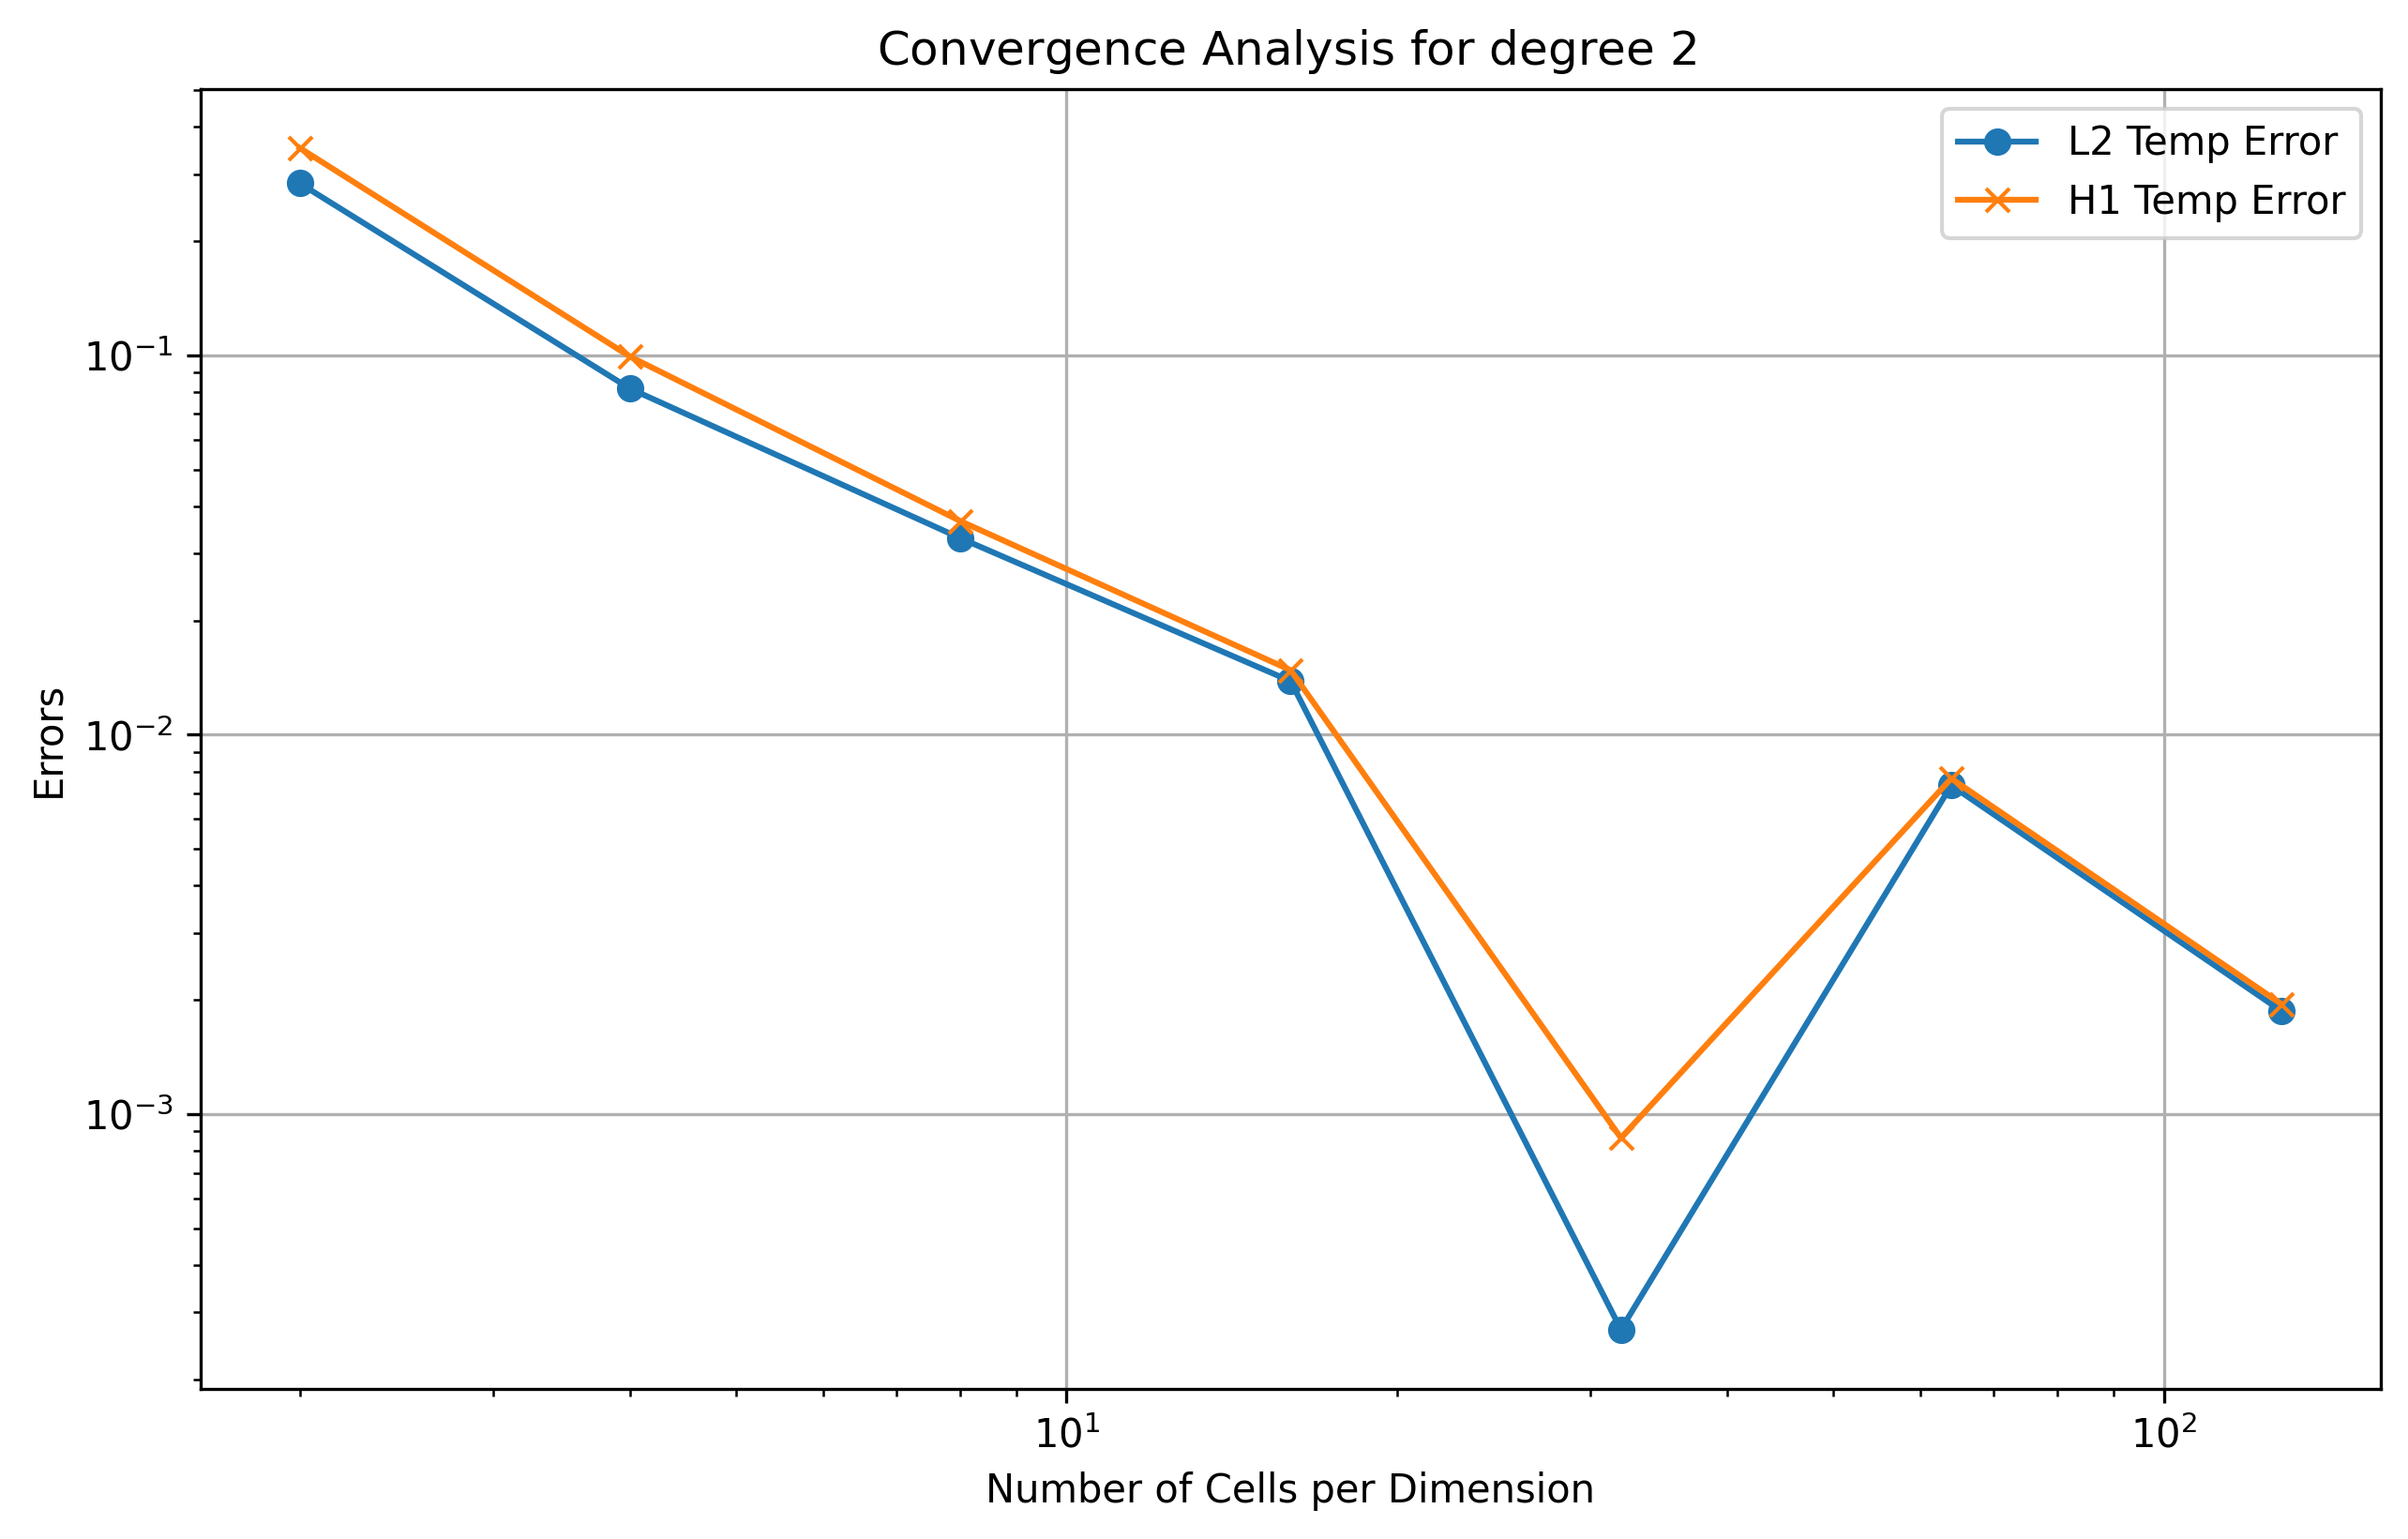
\includegraphics[width=0.6\textwidth]{figures/figures_thermoelas/Temp_X_max=22_Y_max=22_lim=17.0_d=2.png}
	\caption{Error plot of the temperature field ($\|T - T^h\|_{L^2(\Omega)}$ and $\|T - T^h\|_{H^1(\Omega)}$) with $d=2$ B-splines and $\text{lim} = 17.0$}
	\label{fig:error_temp_d2}
\end{figure}

In this figure, we can observe that the error in the temperature field is decreasing with the number of cells $n_{\text{cells}}$ until $n_{\text{cells}} = 32$. After that, the error is increasing and decreases again. This behavior is likely due to the interaction between the mesh refinement, the B-spline approximation properties and the properties of the medium. When the degree of the B-splines is set to 3, we can see in figure \ref{fig:error_temp_d3} that the hollow moves to a lower number of cells.

\begin{figure}[!h]
	\centering
	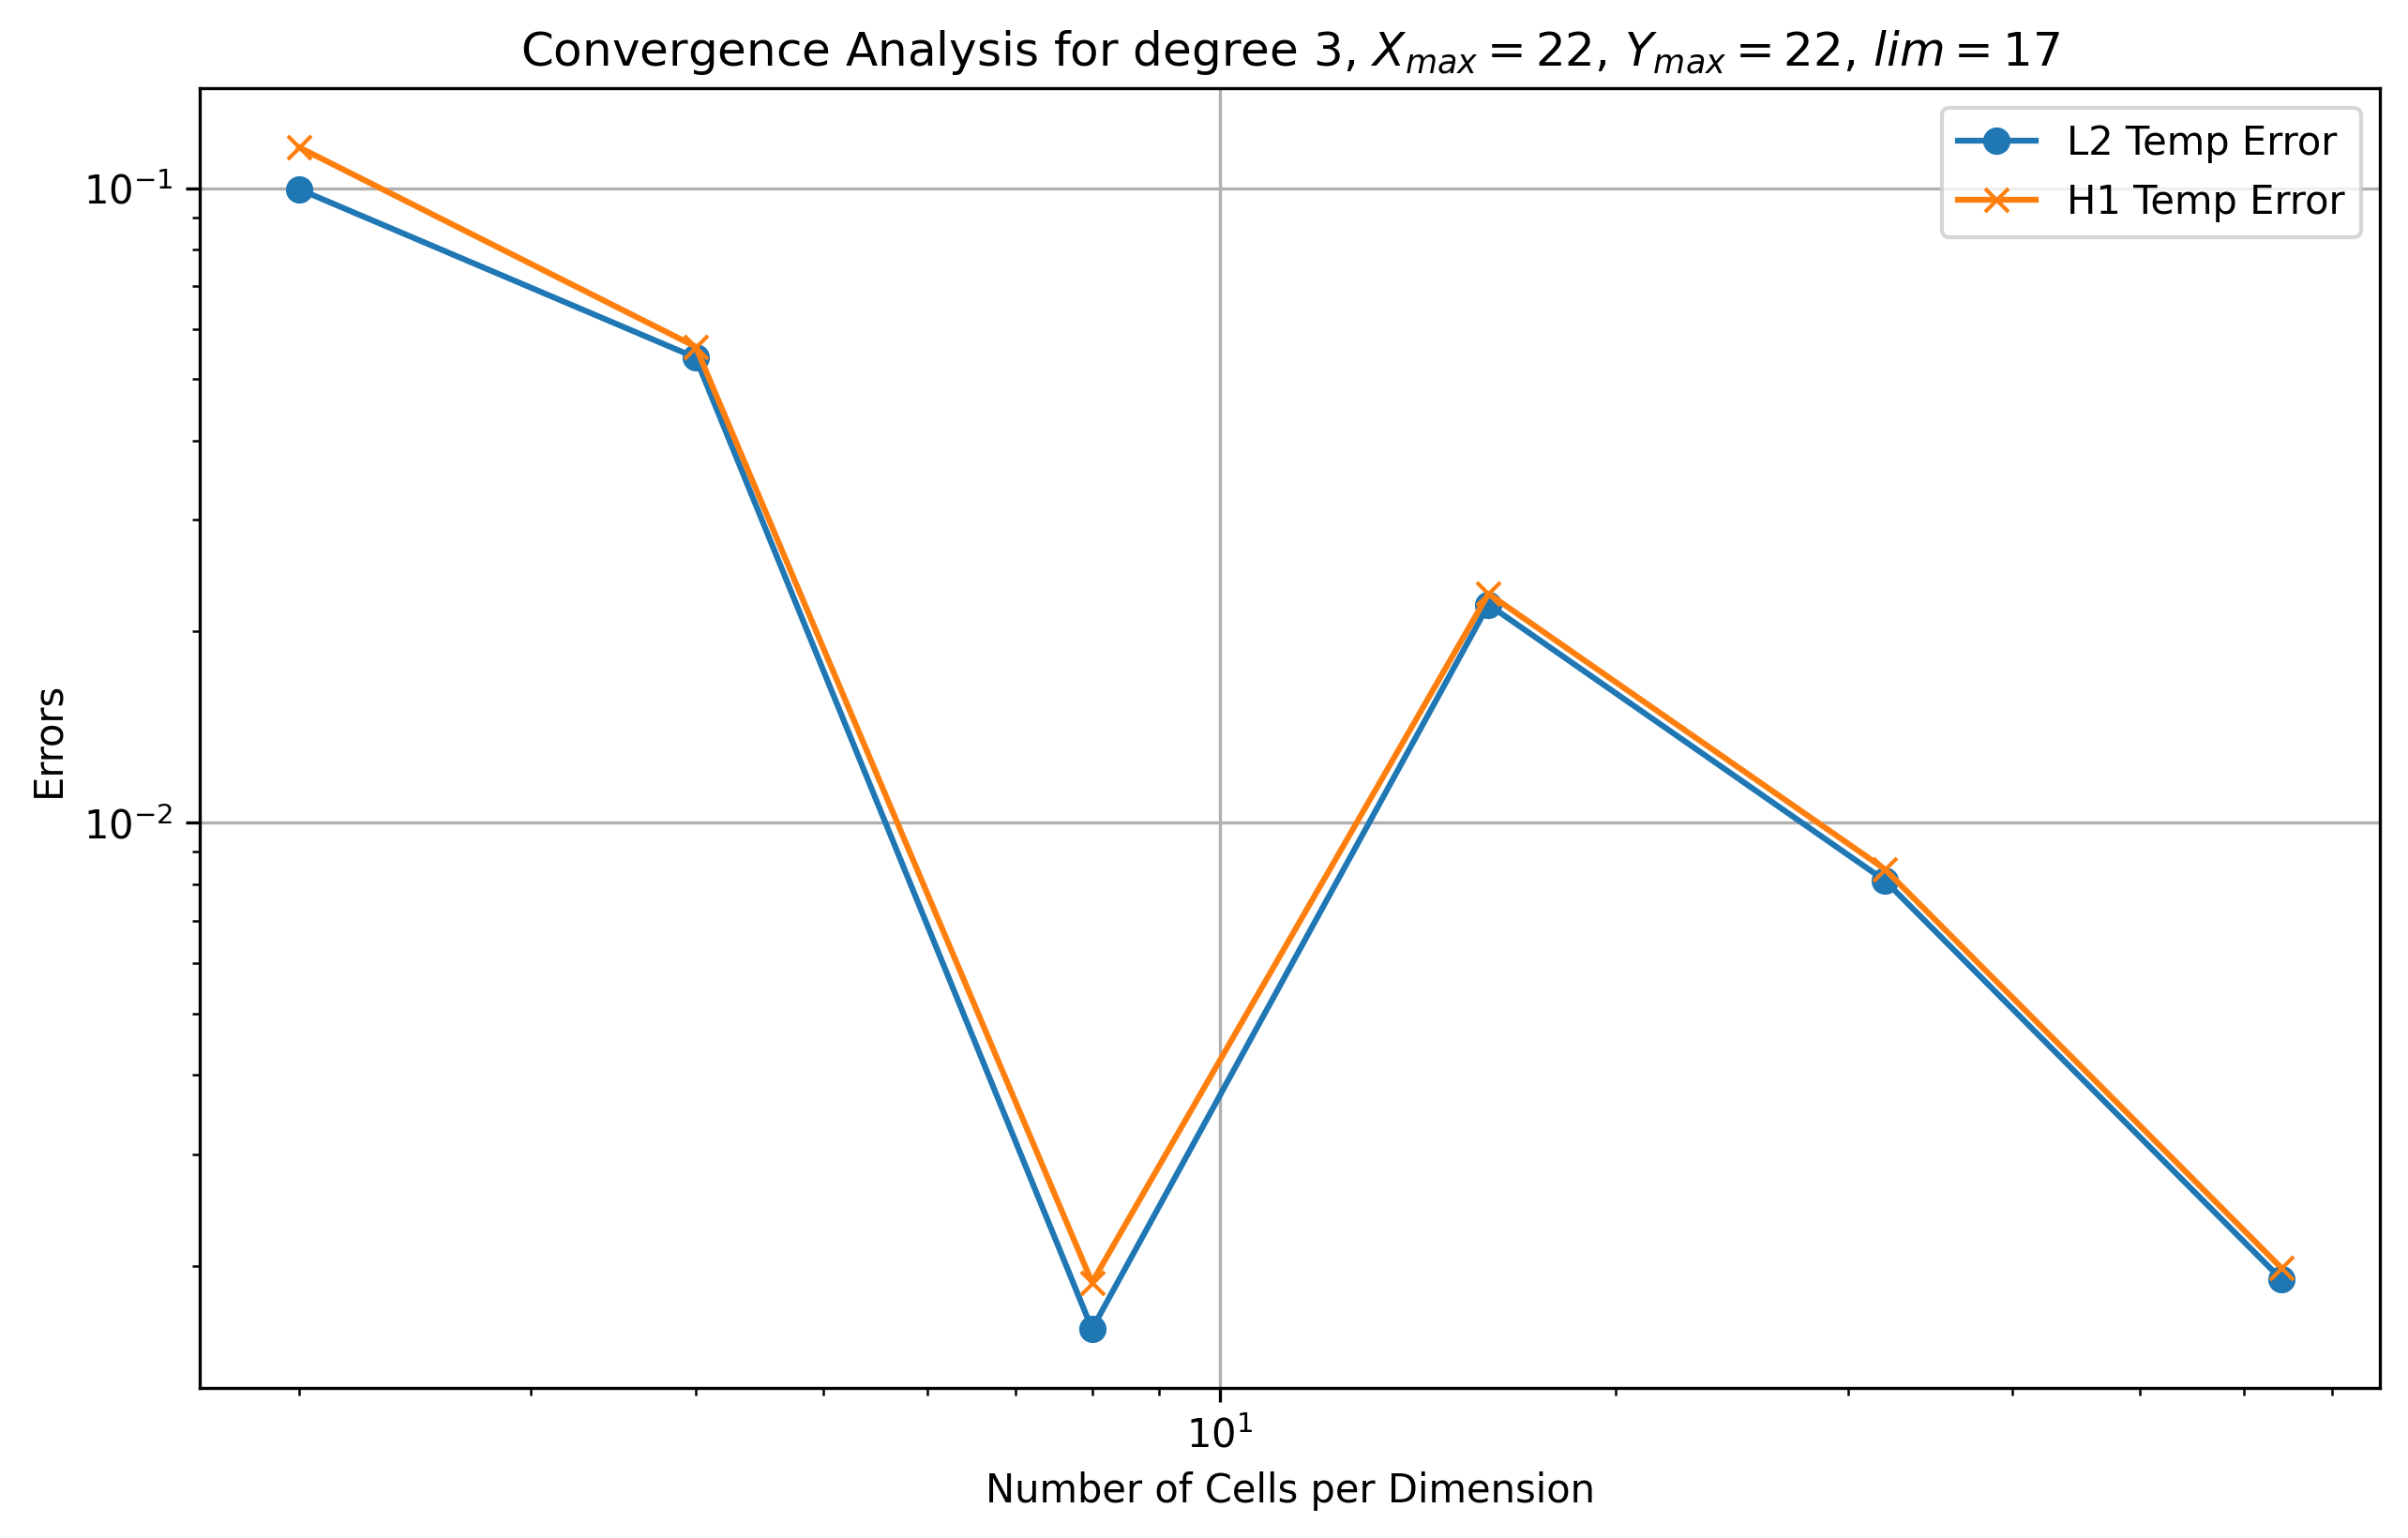
\includegraphics[width=0.6\textwidth]{figures/figures_thermoelas/Temp_X_max=22_Y_max=22_lim=17_d=3.png}
	\caption{Error plot of the temperature field ($\|T - T^h\|_{L^2(\Omega)}$ and $\|T - T^h\|_{H^1(\Omega)}$) with $d=3$ B-splines and $\text{lim} = 17.0$}
	\label{fig:error_temp_d3}
\end{figure}

The same phenomenon is observed for the displacement field.
One reason that can explain this phenomenon is the placement of the B-spline knots and the corresponding basis functions. As the mesh is refined, the B-spline basis functions become more localized, which can lead to better approximation properties in certain regions of the domain. In the medium that we are considering, the line $y = \text{lim} = 17.0$ plays a crucial role in the behavior of the solution because it corresponds to a significant change in the material properties. Moreover, \texttt{PSYDAC} cannot handle coefficients defined piecewise so it is necessary to use an approximation of Heaviside functions to define coefficients. For example, $\lambda(y)$ is defined by:
$$ \lambda(y) = \big( (\lambda_W - \lambda_{Cu}) \frac{x}{\text{lim}} + \lambda_{Cu} \big) \text{H}(\text{lim}-x) + \lambda_{W} \text{H}(x-\text{lim}) \qquad H \text{ is the Heaviside function}.$$
One hypothesis that can be made to verify the role of the line $y = \text{lim}$ is to move its value up and down and observe the effect on the solution. Especially, it's possible to move the value of $\text{lim}$ to $16.5$. This value corresponds to lines with breakpoints when the domain $\Omega$ is discretized into different cells. 
\begin{figure}[!h]
	\begin{subfigure}[b]{0.49\textwidth}
		\centering
		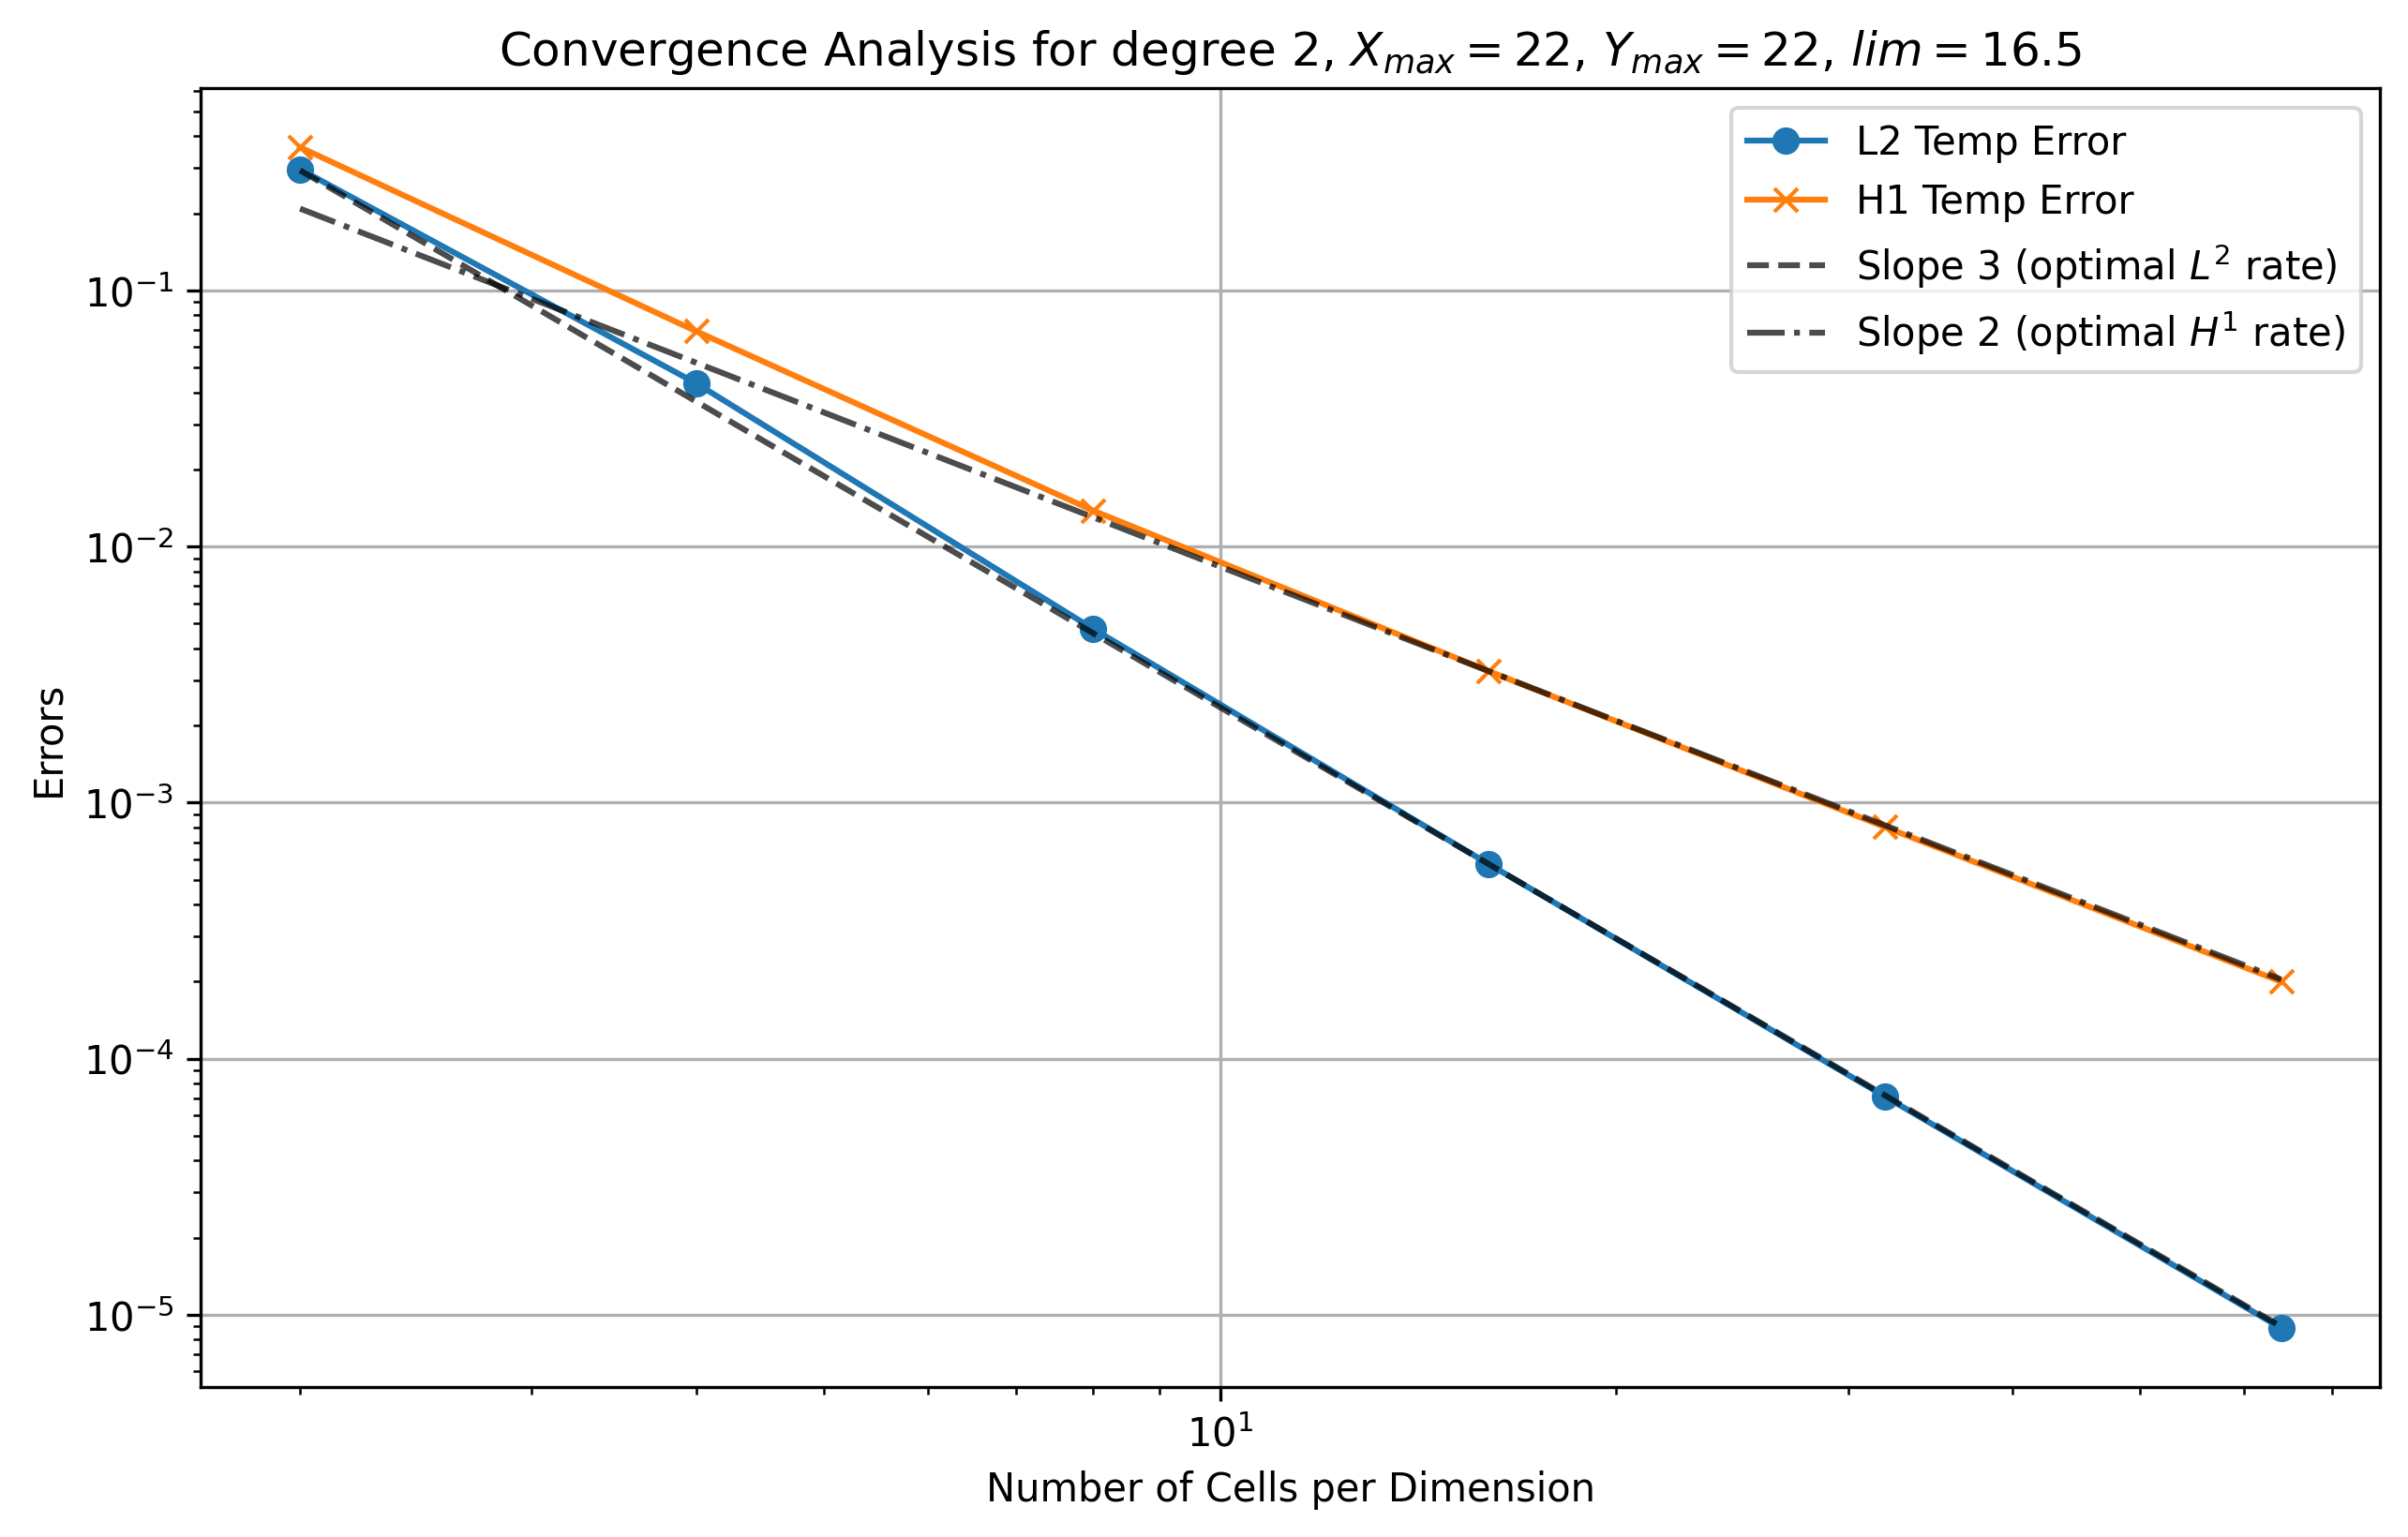
\includegraphics[width=\textwidth]{figures/figures_thermoelas/Temp_X_max=22_Y_max=22_lim=16.5_d=2.png}
		\caption{Error plot of the temperature field}
		\label{fig:error_temp_d2_lim_16_5}
	\end{subfigure}
	\begin{subfigure}[b]{0.49\textwidth}
		\centering
		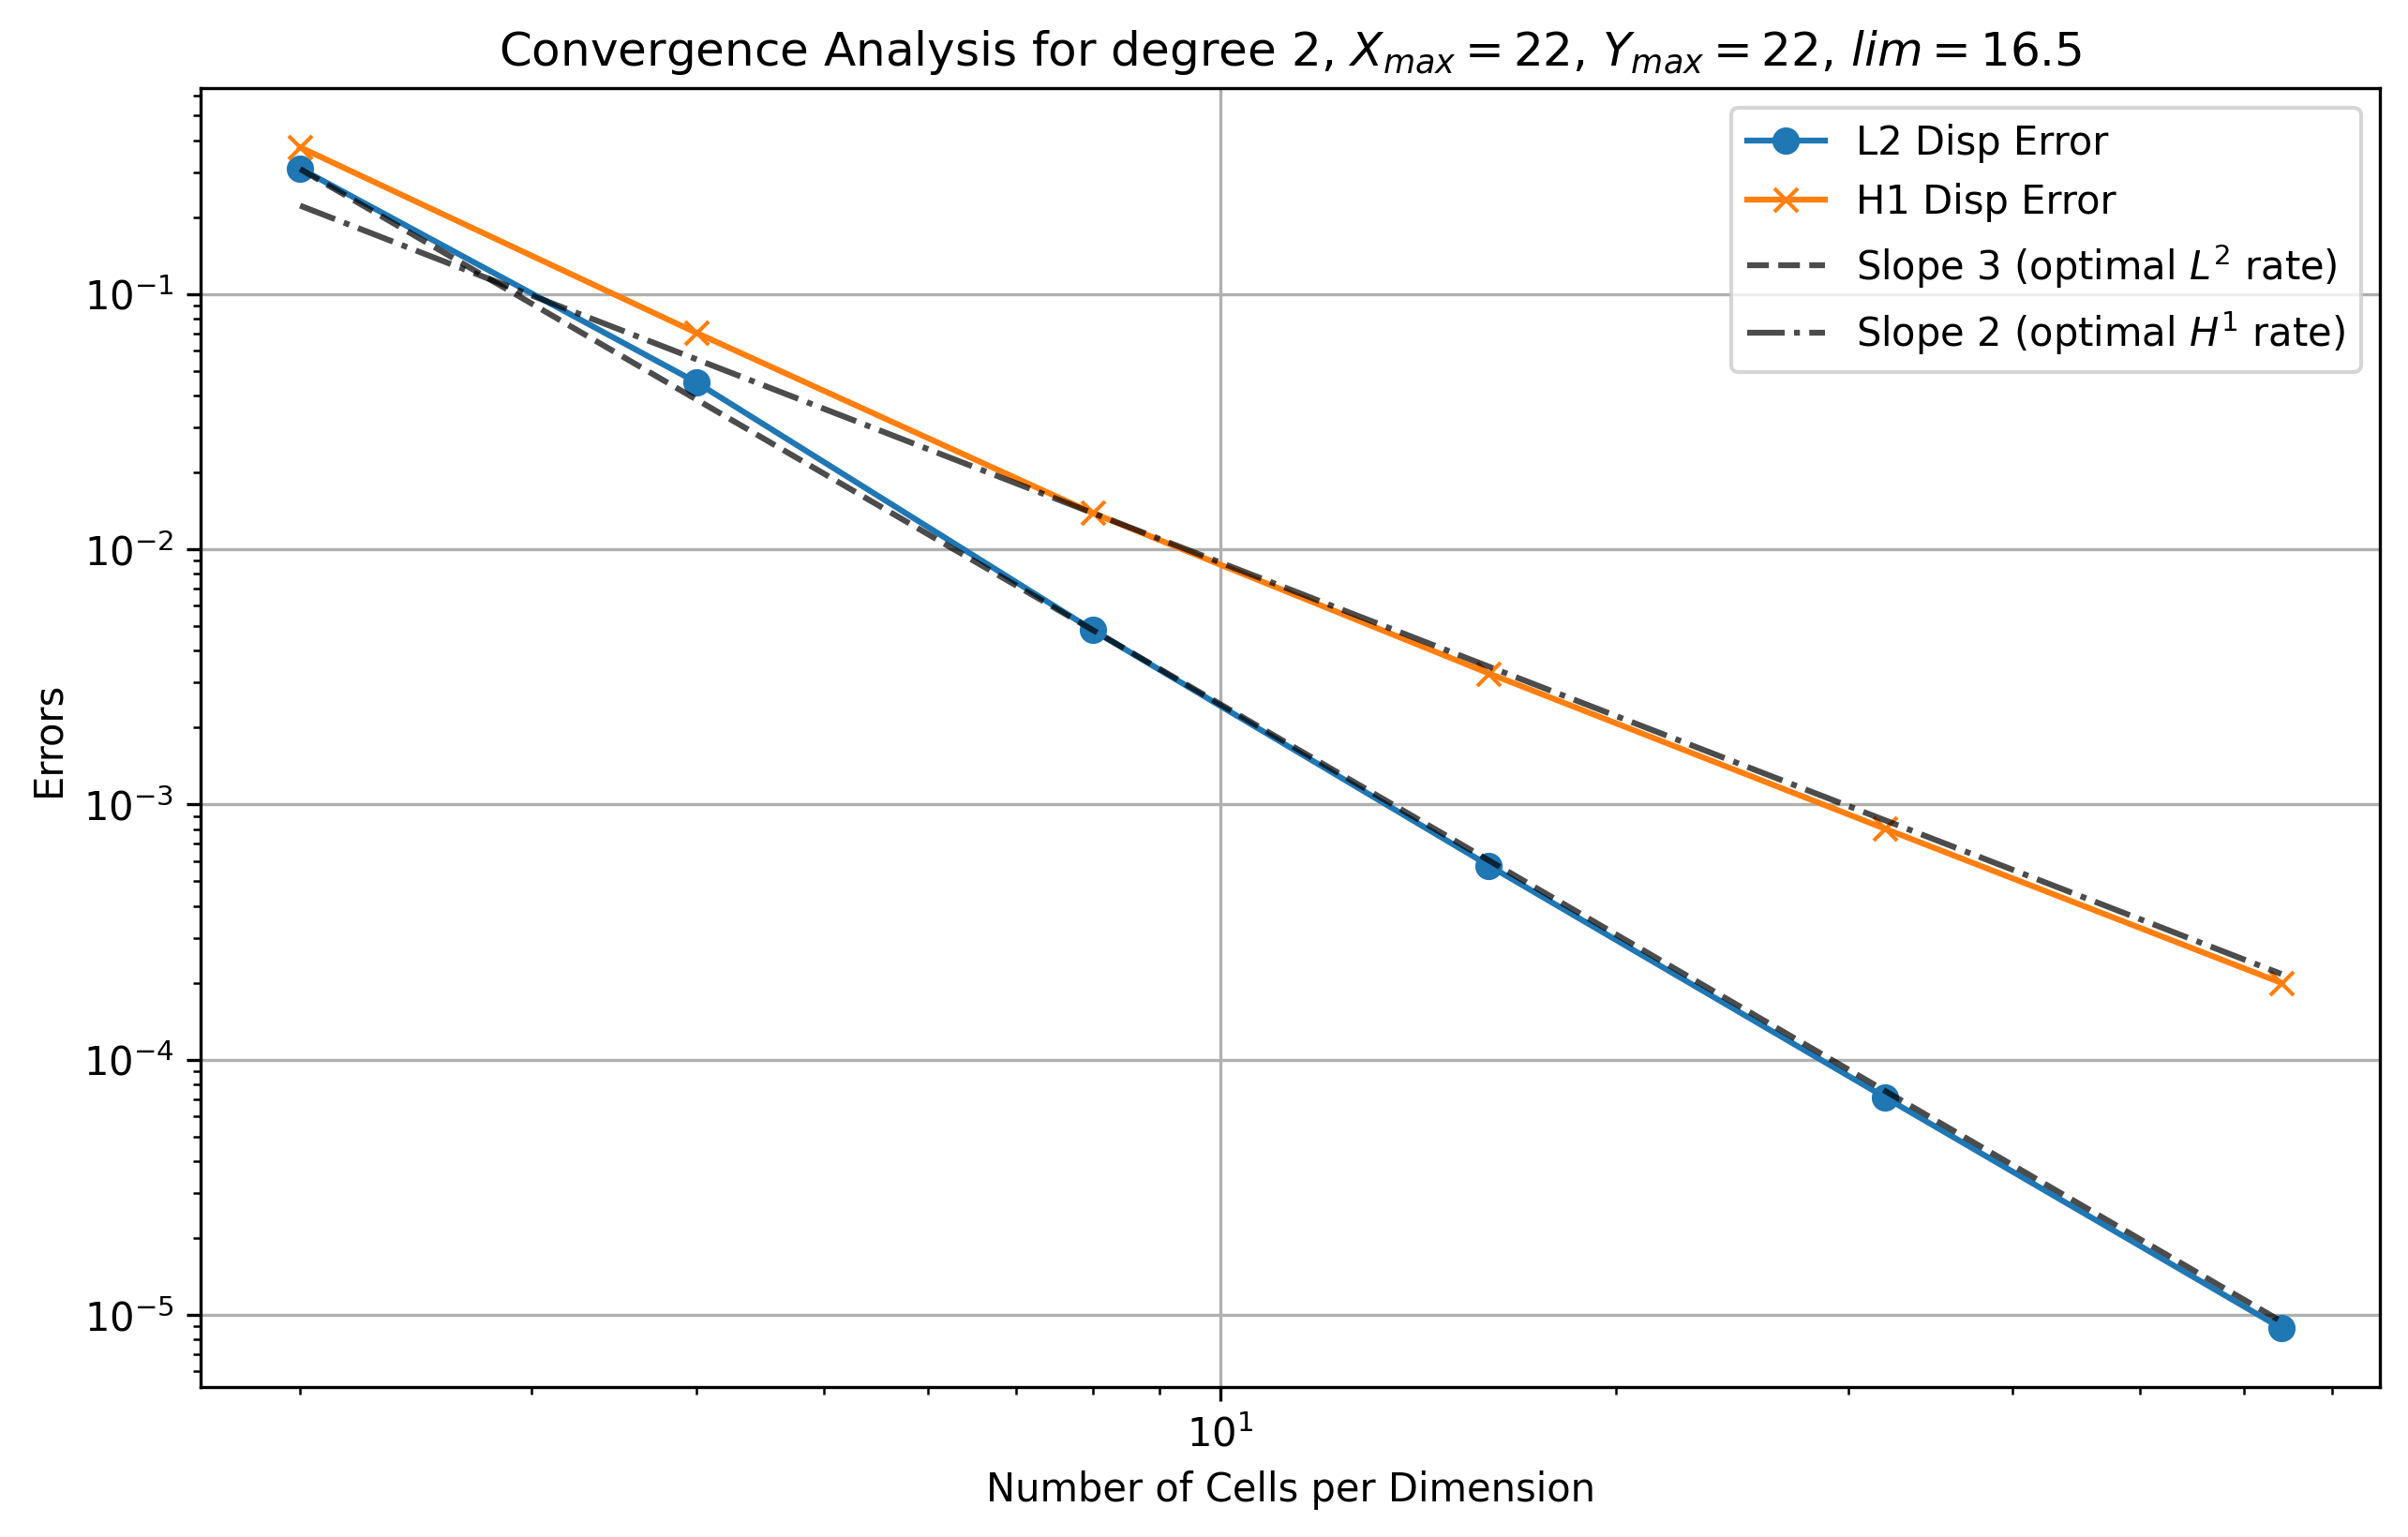
\includegraphics[width=\textwidth]{figures/figures_thermoelas/Disp_X_max=22_Y_max=22_lim=16.5_d=2_disp.png}
		\caption{Error plot of the displacement field}
		\label{fig:error_disp_d2_lim_16_5}
	\end{subfigure}
	\caption{Error plots with $\text{lim} = 16.5$ and degree 2 B-splines}
\end{figure}

In this case, we can observe the optimal convergence behavior of the error as predicted by the theory. So the position of the line $y = \text{lim}$ is crucial for the accuracy of the solution and the simulation.
To make the simulation possible in the case described in subsection \ref{subsec:problem_setup_parameters}, we need to get a simulation setup that solves the problem when $\text{lim} = 17$.
For the moment, the function which discretizes the domain and creates the finite dimensional spline space takes only the number of cells per direction as argument. I have implemented a new feature to the library which allows the user to provide a custom discretization grid. This feature required adding new functions to the \texttt{Geometry} class and modifying the previous \texttt{discretize} function in \texttt{PSYDAC}. To ensure the correct working of this new feature, I have also implemented a set of unit tests.
\begin{figure}[!h]
	\centering
	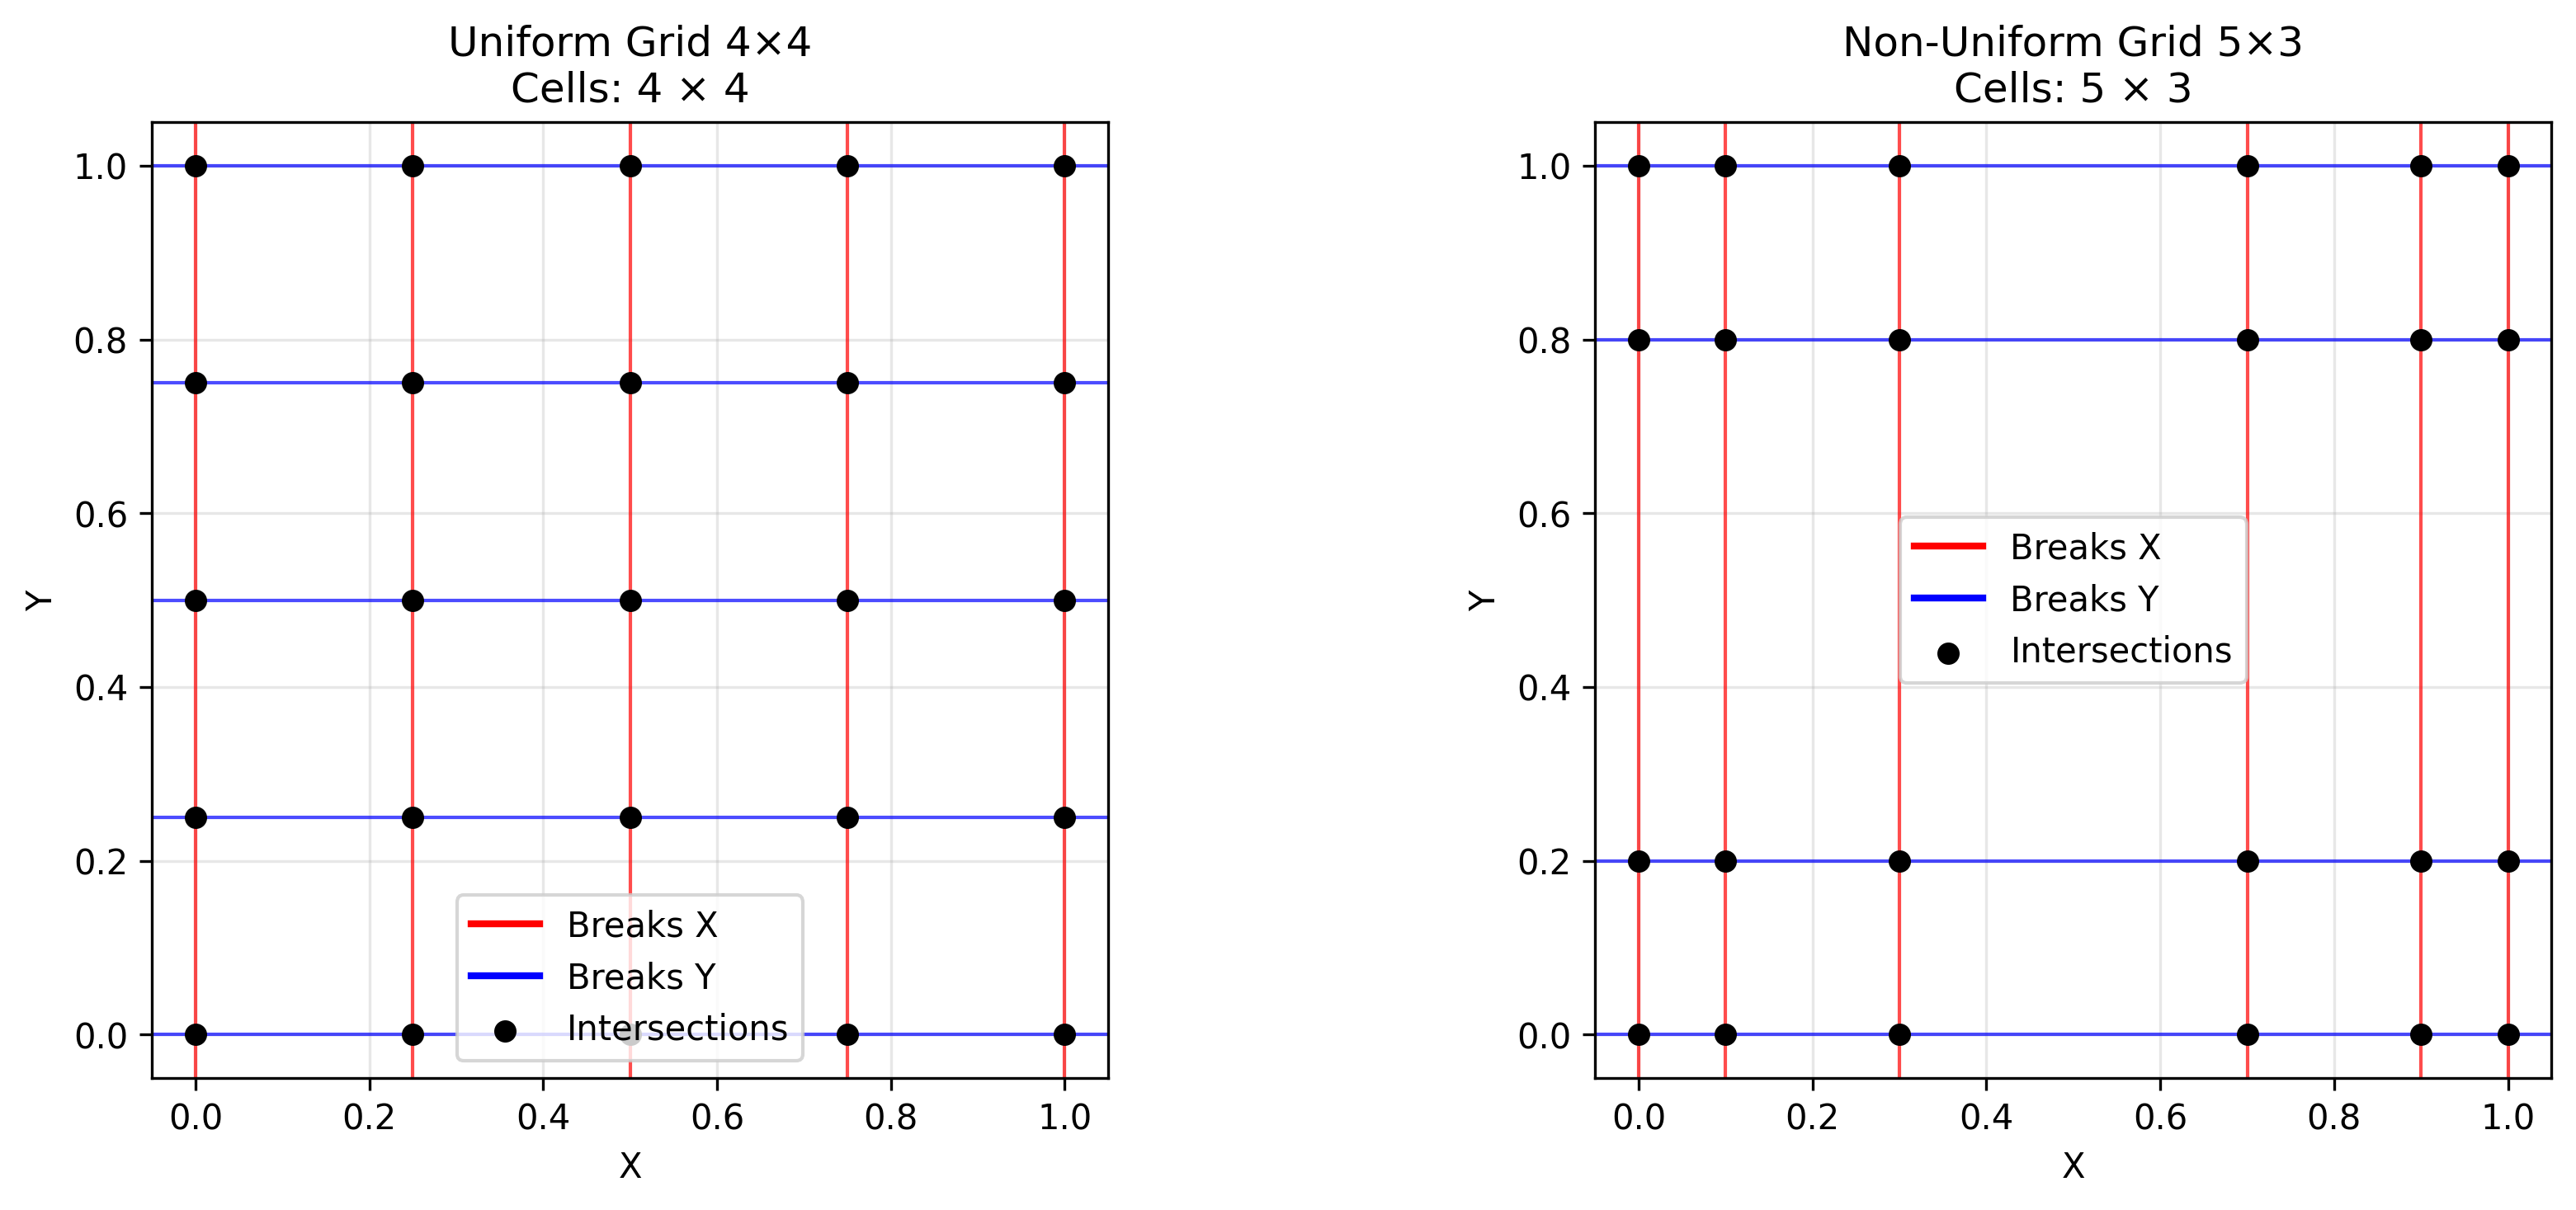
\includegraphics[width=0.8\textwidth]{figures/custom_grid.png}
	\caption{Example of a custom discretization grid}
	\label{fig:custom_grid_example}
\end{figure}
This new feature allows the user to define a custom grid for the discretization of the domain. A complete description of this feature is available on GitHub: \href{https://github.com/pyccel/psydac/pull/518}{https://github.com/pyccel/psydac/pull/518}

With this feature, we can now simulate correctly the problem when $\text{lim} = 17$ as it was described in the simplified problem setup. The results are shown in the figures below.
\begin{figure}[!h]
	\begin{subfigure}[b]{0.49\textwidth}
		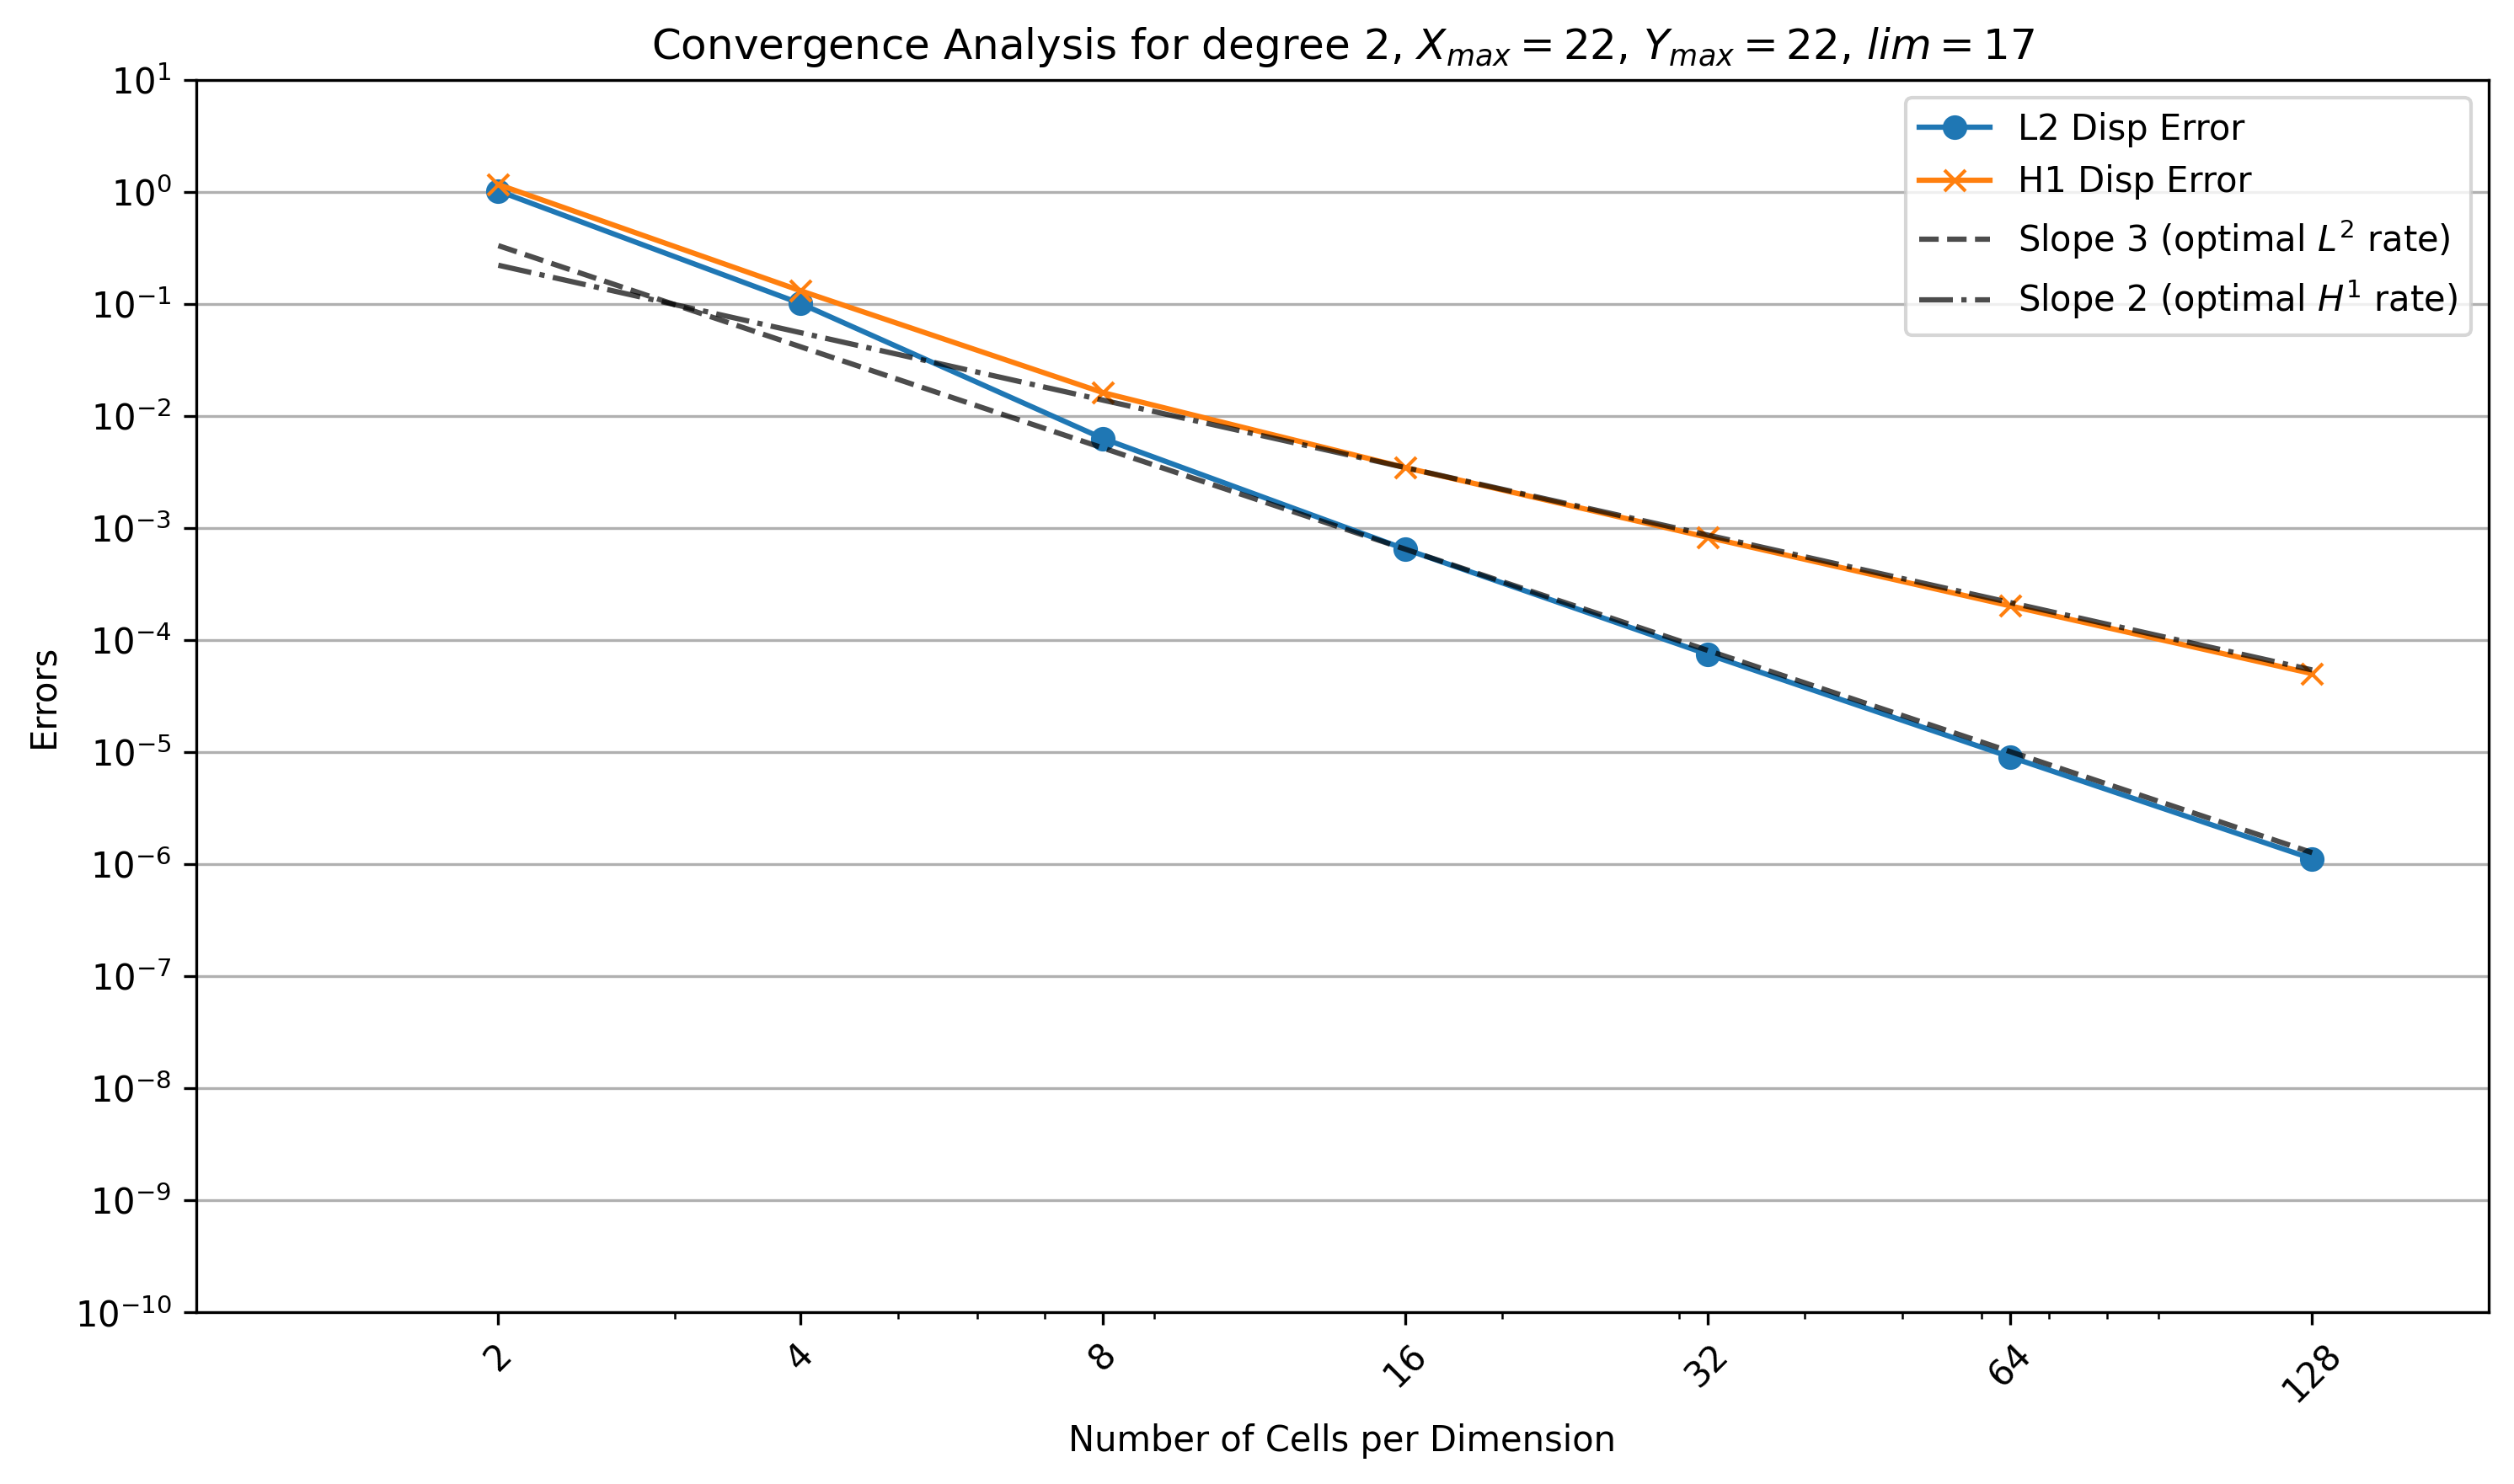
\includegraphics[width=\textwidth]{figures/figures_thermoelas_degree/Disp_X_max=22_Y_max=22_lim=17_d=2_disp.png}
		\caption{Displacement field for degree 2 B-splines}
		\label{fig:disp_d2_lim_17}
	\end{subfigure}
	\begin{subfigure}[b]{0.49\textwidth}
		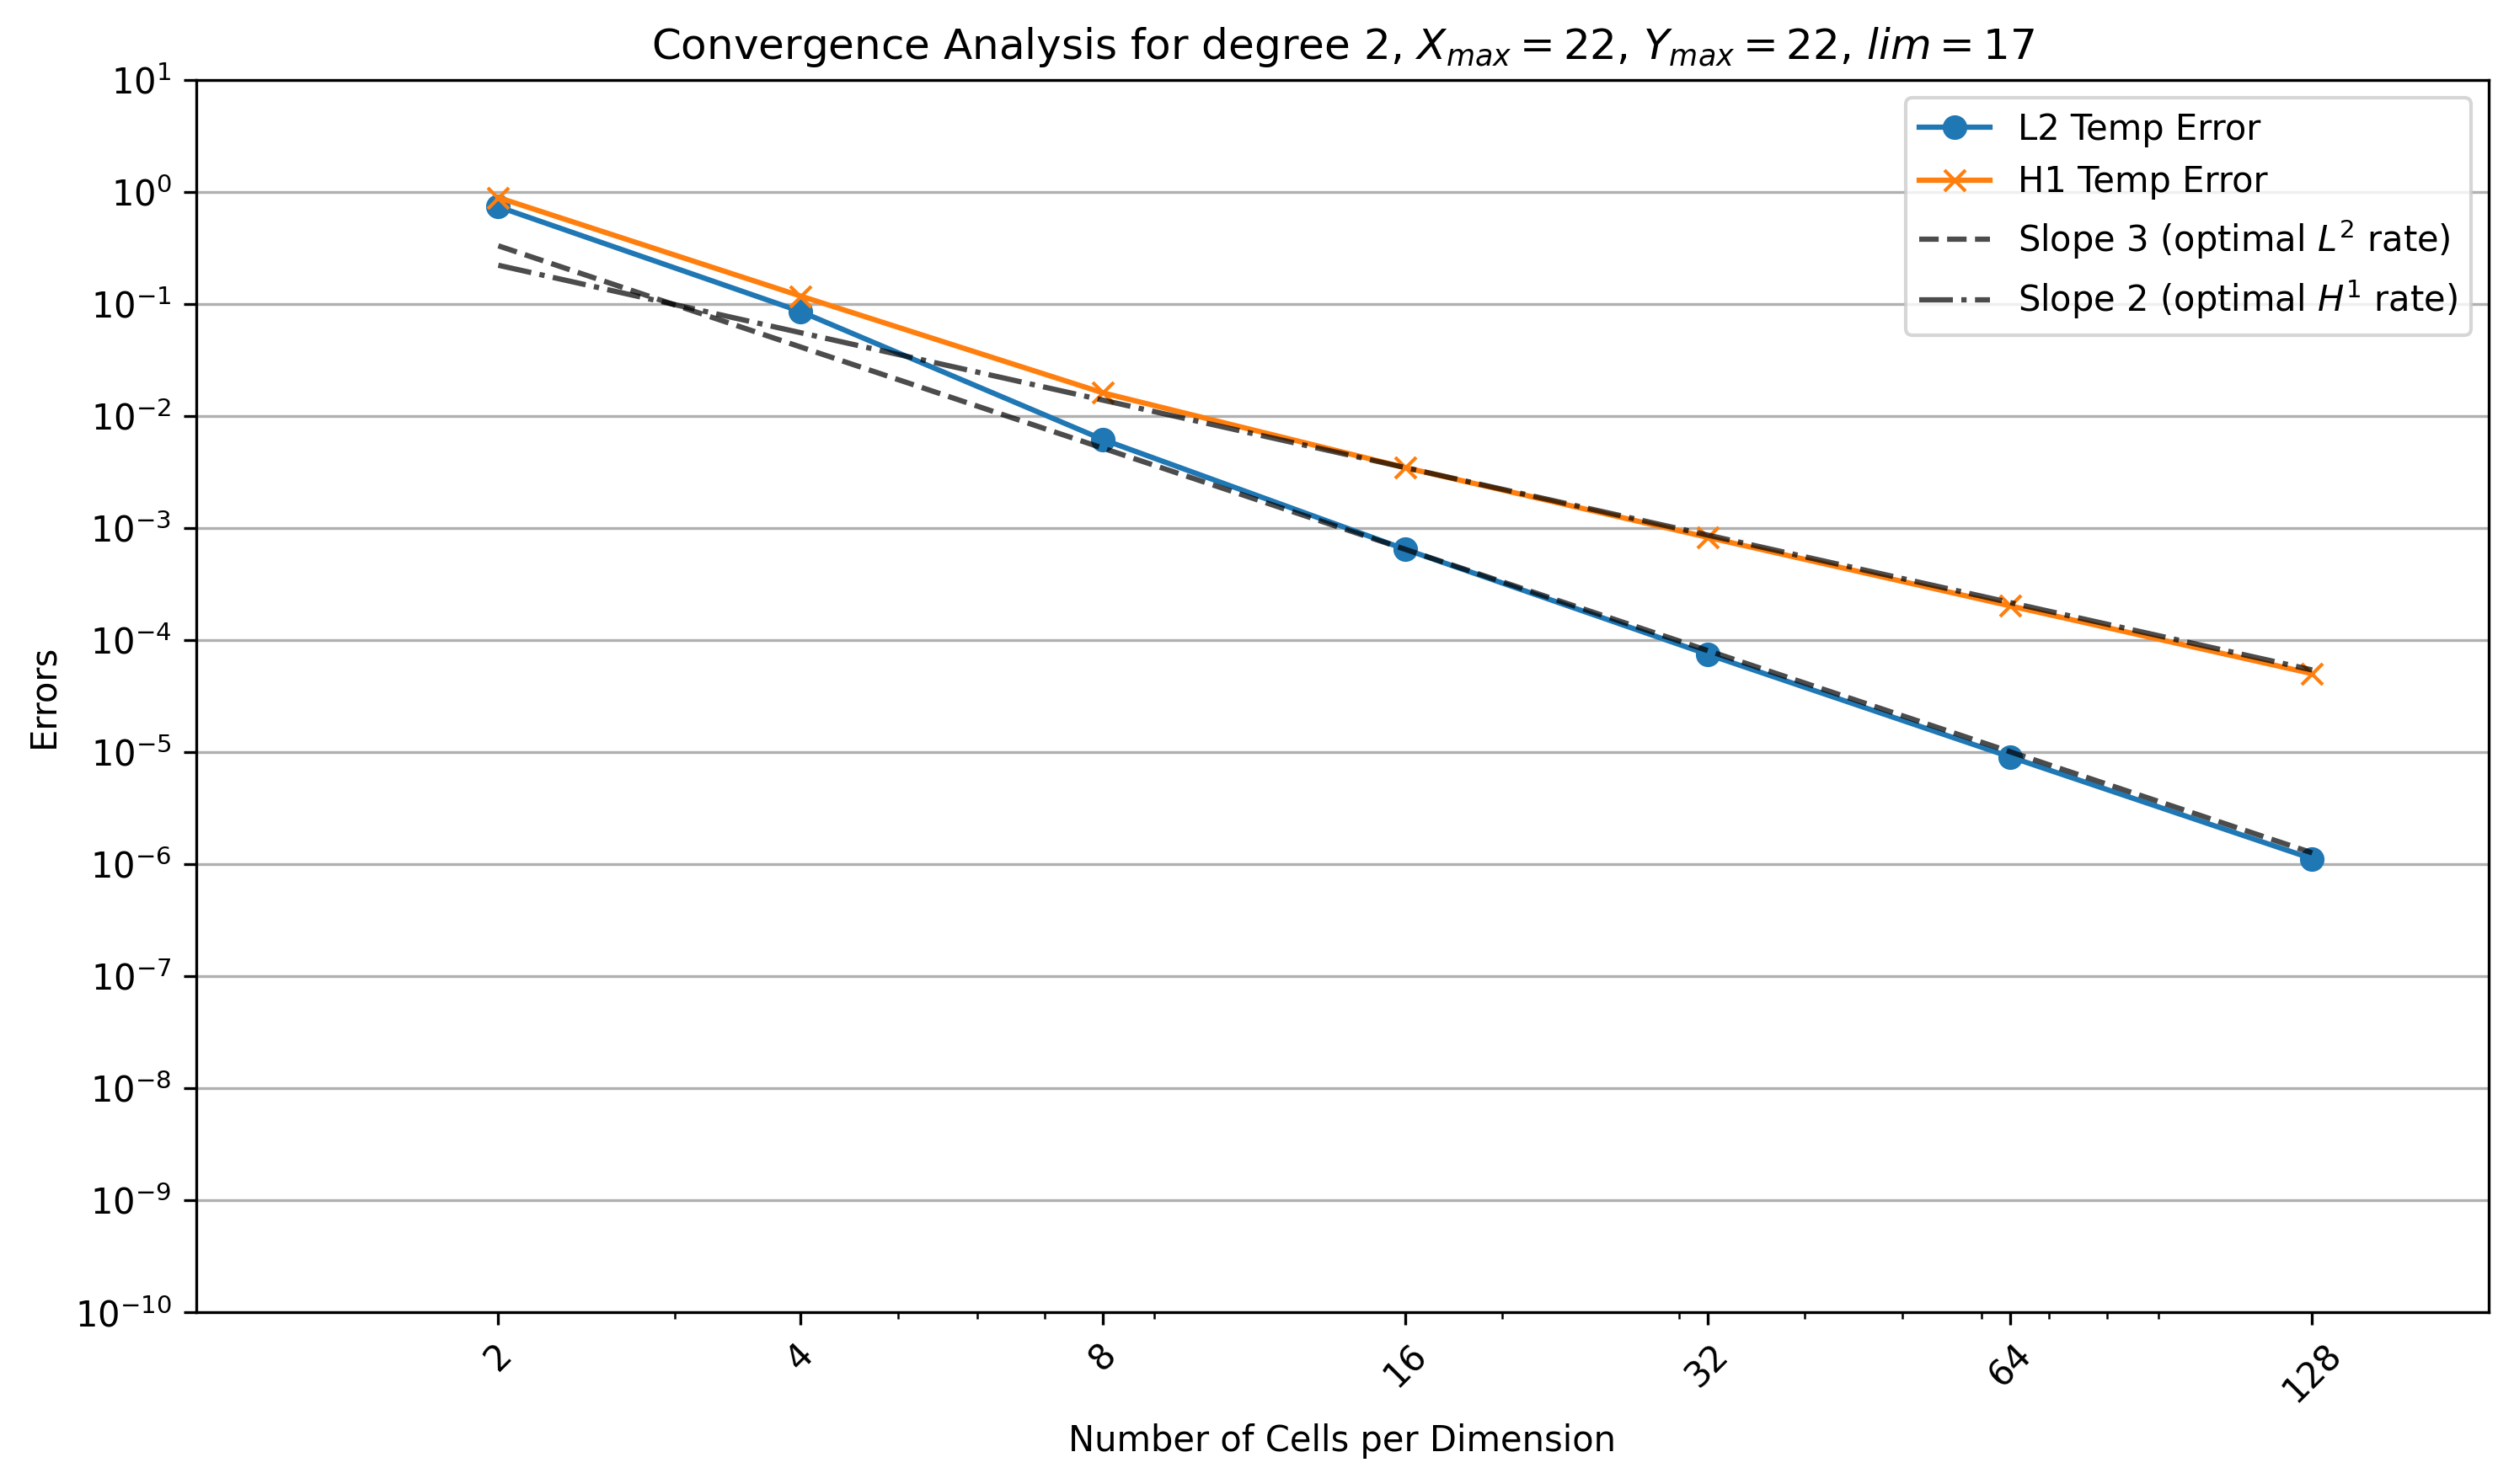
\includegraphics[width=\textwidth]{figures/figures_thermoelas_degree/Temp_X_max=22_Y_max=22_lim=17_d=2.png}
		\caption{Temperature field for degree 2 B-splines}
		\label{fig:temp_d2_lim_17}
	\end{subfigure}
	\begin{subfigure}[b]{0.49\textwidth}
		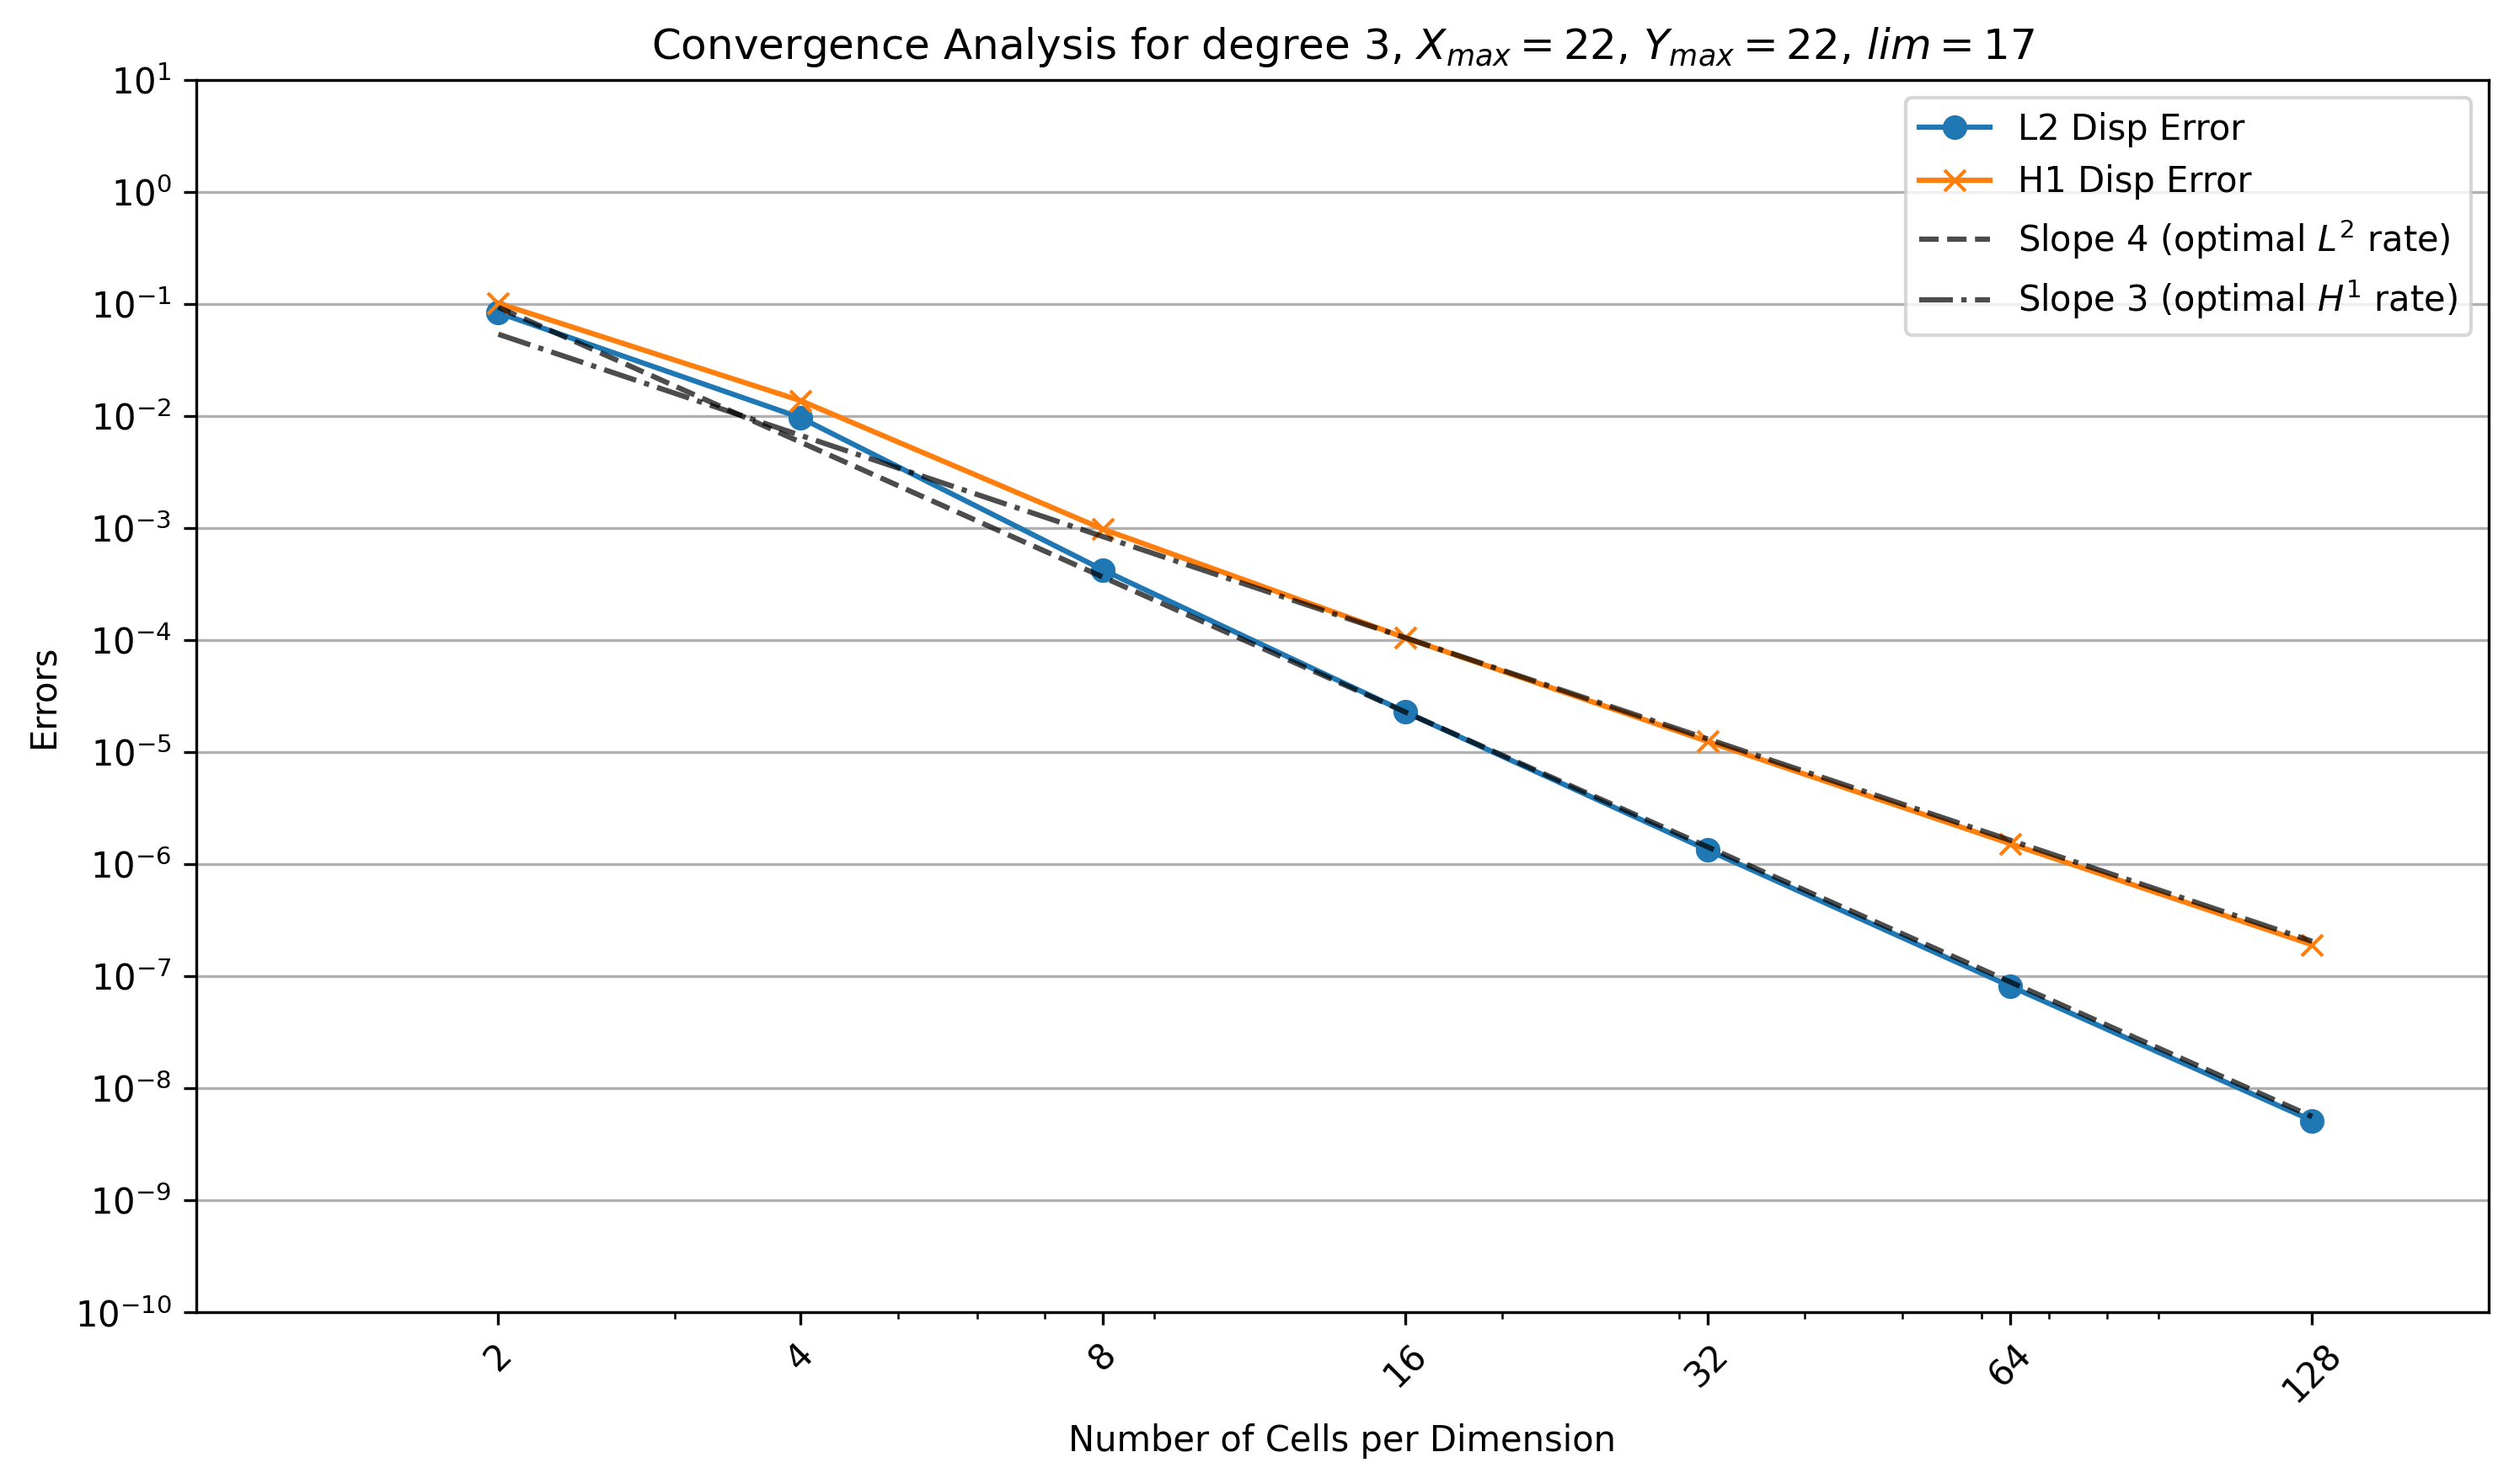
\includegraphics[width=\textwidth]{figures/figures_thermoelas_degree/Disp_X_max=22_Y_max=22_lim=17_d=3_disp.png}
		\caption{Displacement field for degree 3 B-splines}
		\label{fig:disp_d3_lim_17}
	\end{subfigure}
	\begin{subfigure}[b]{0.49\textwidth}
		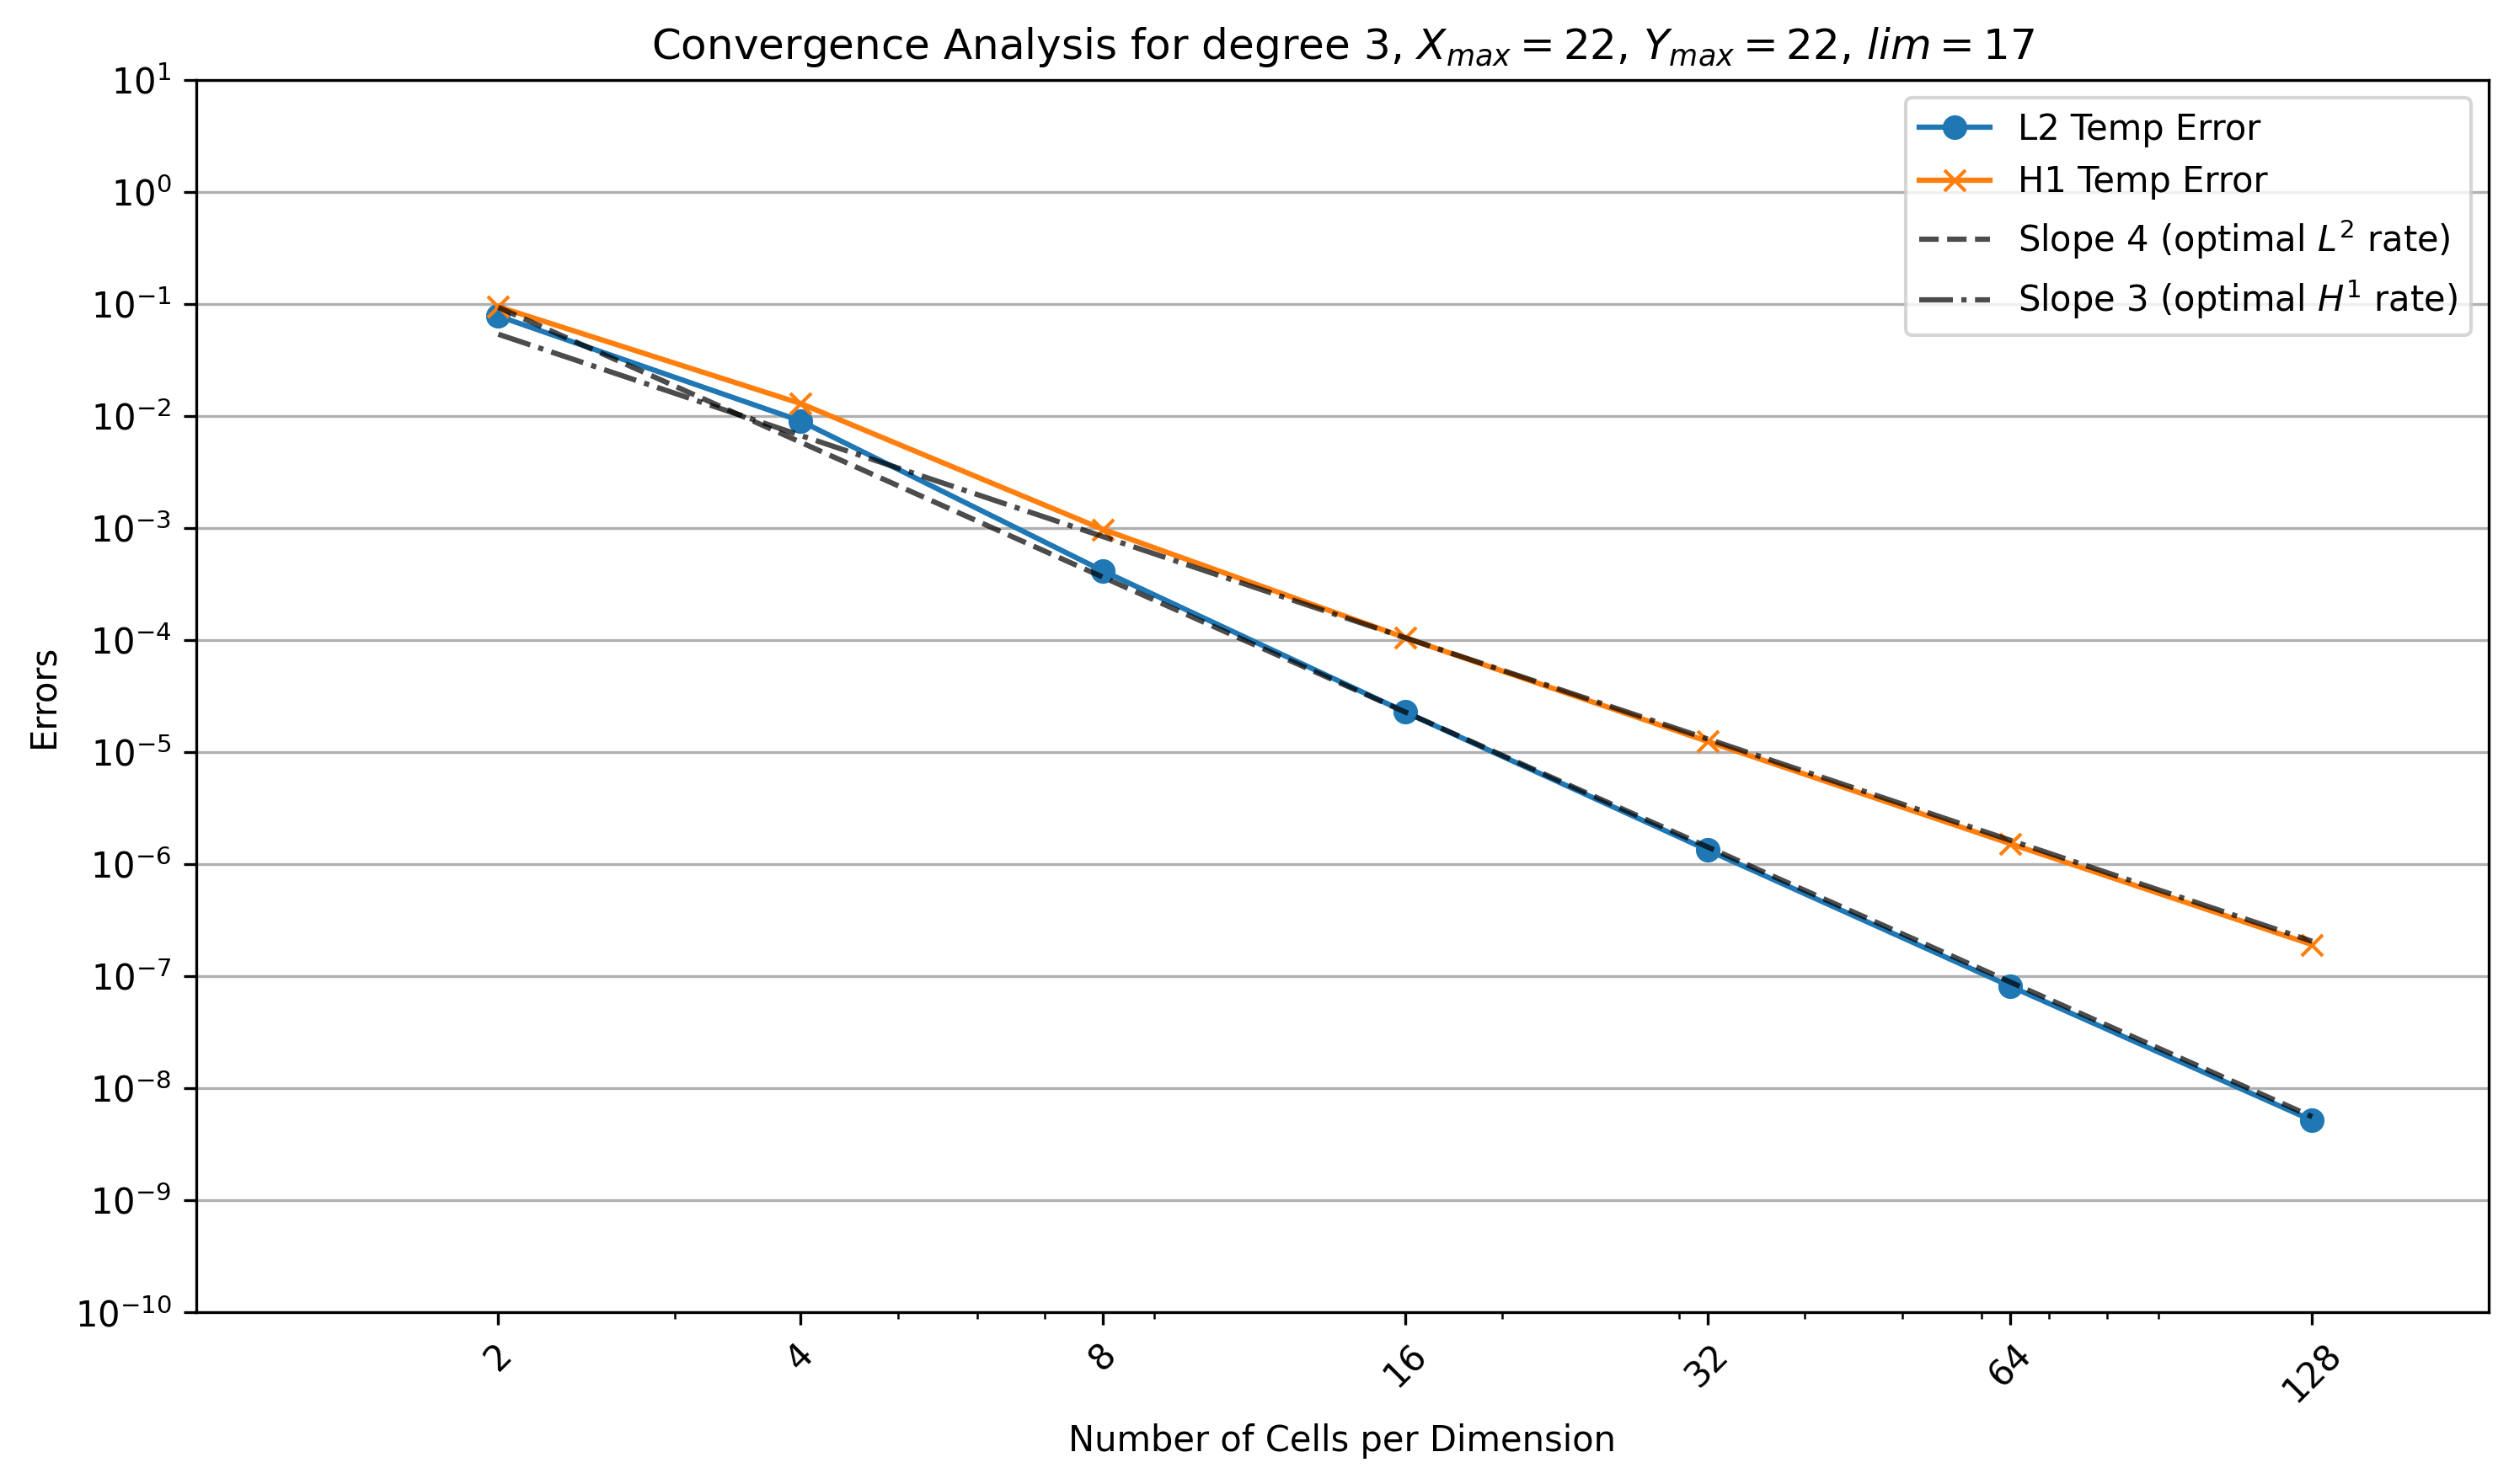
\includegraphics[width=\textwidth]{figures/figures_thermoelas_degree/Temp_X_max=22_Y_max=22_lim=17_d=3.png}
		\caption{Temperature field for degree 3 B-splines}
		\label{fig:temp_d3_lim_17}
	\end{subfigure}
\end{figure}
\newpage
\begin{figure}[!h]\ContinuedFloat
	\begin{subfigure}[b]{0.49\textwidth}
		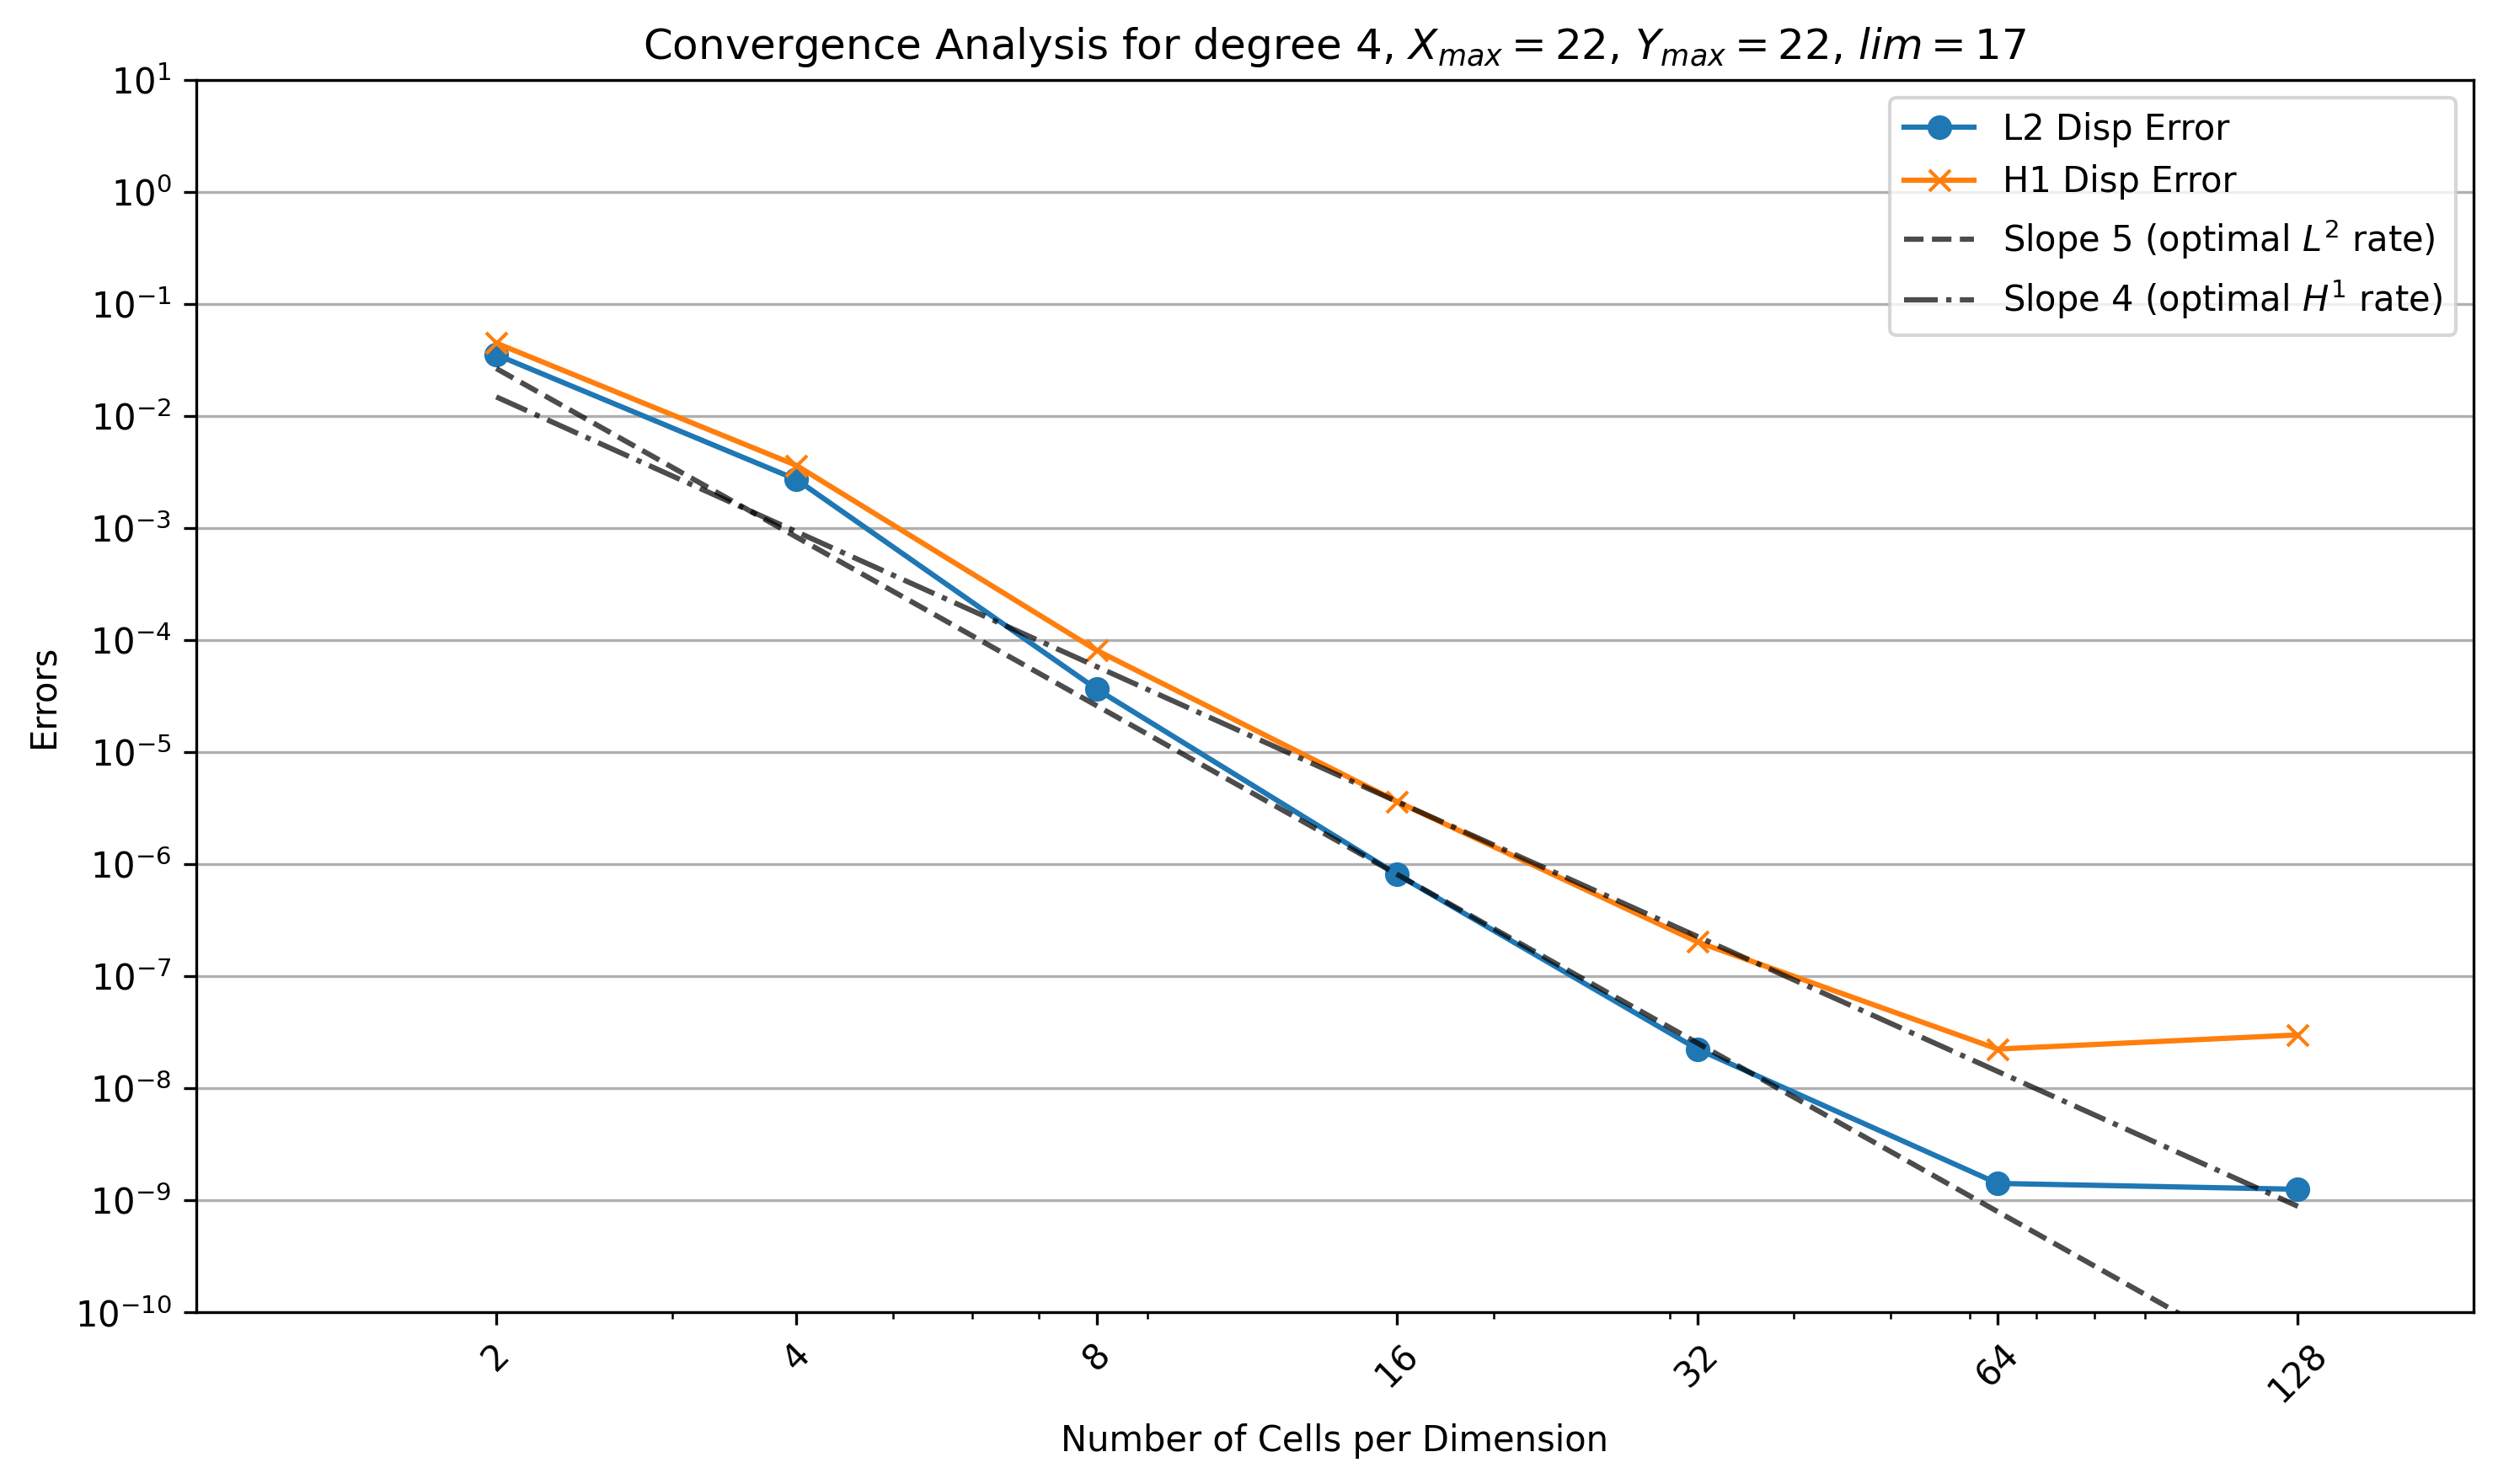
\includegraphics[width=\textwidth]{figures/figures_thermoelas_degree/Disp_X_max=22_Y_max=22_lim=17_d=4_disp.png}
		\caption{Displacement field for degree 4 B-splines}
		\label{fig:disp_d4_lim_17}
	\end{subfigure}
	\begin{subfigure}[b]{0.49\textwidth}
		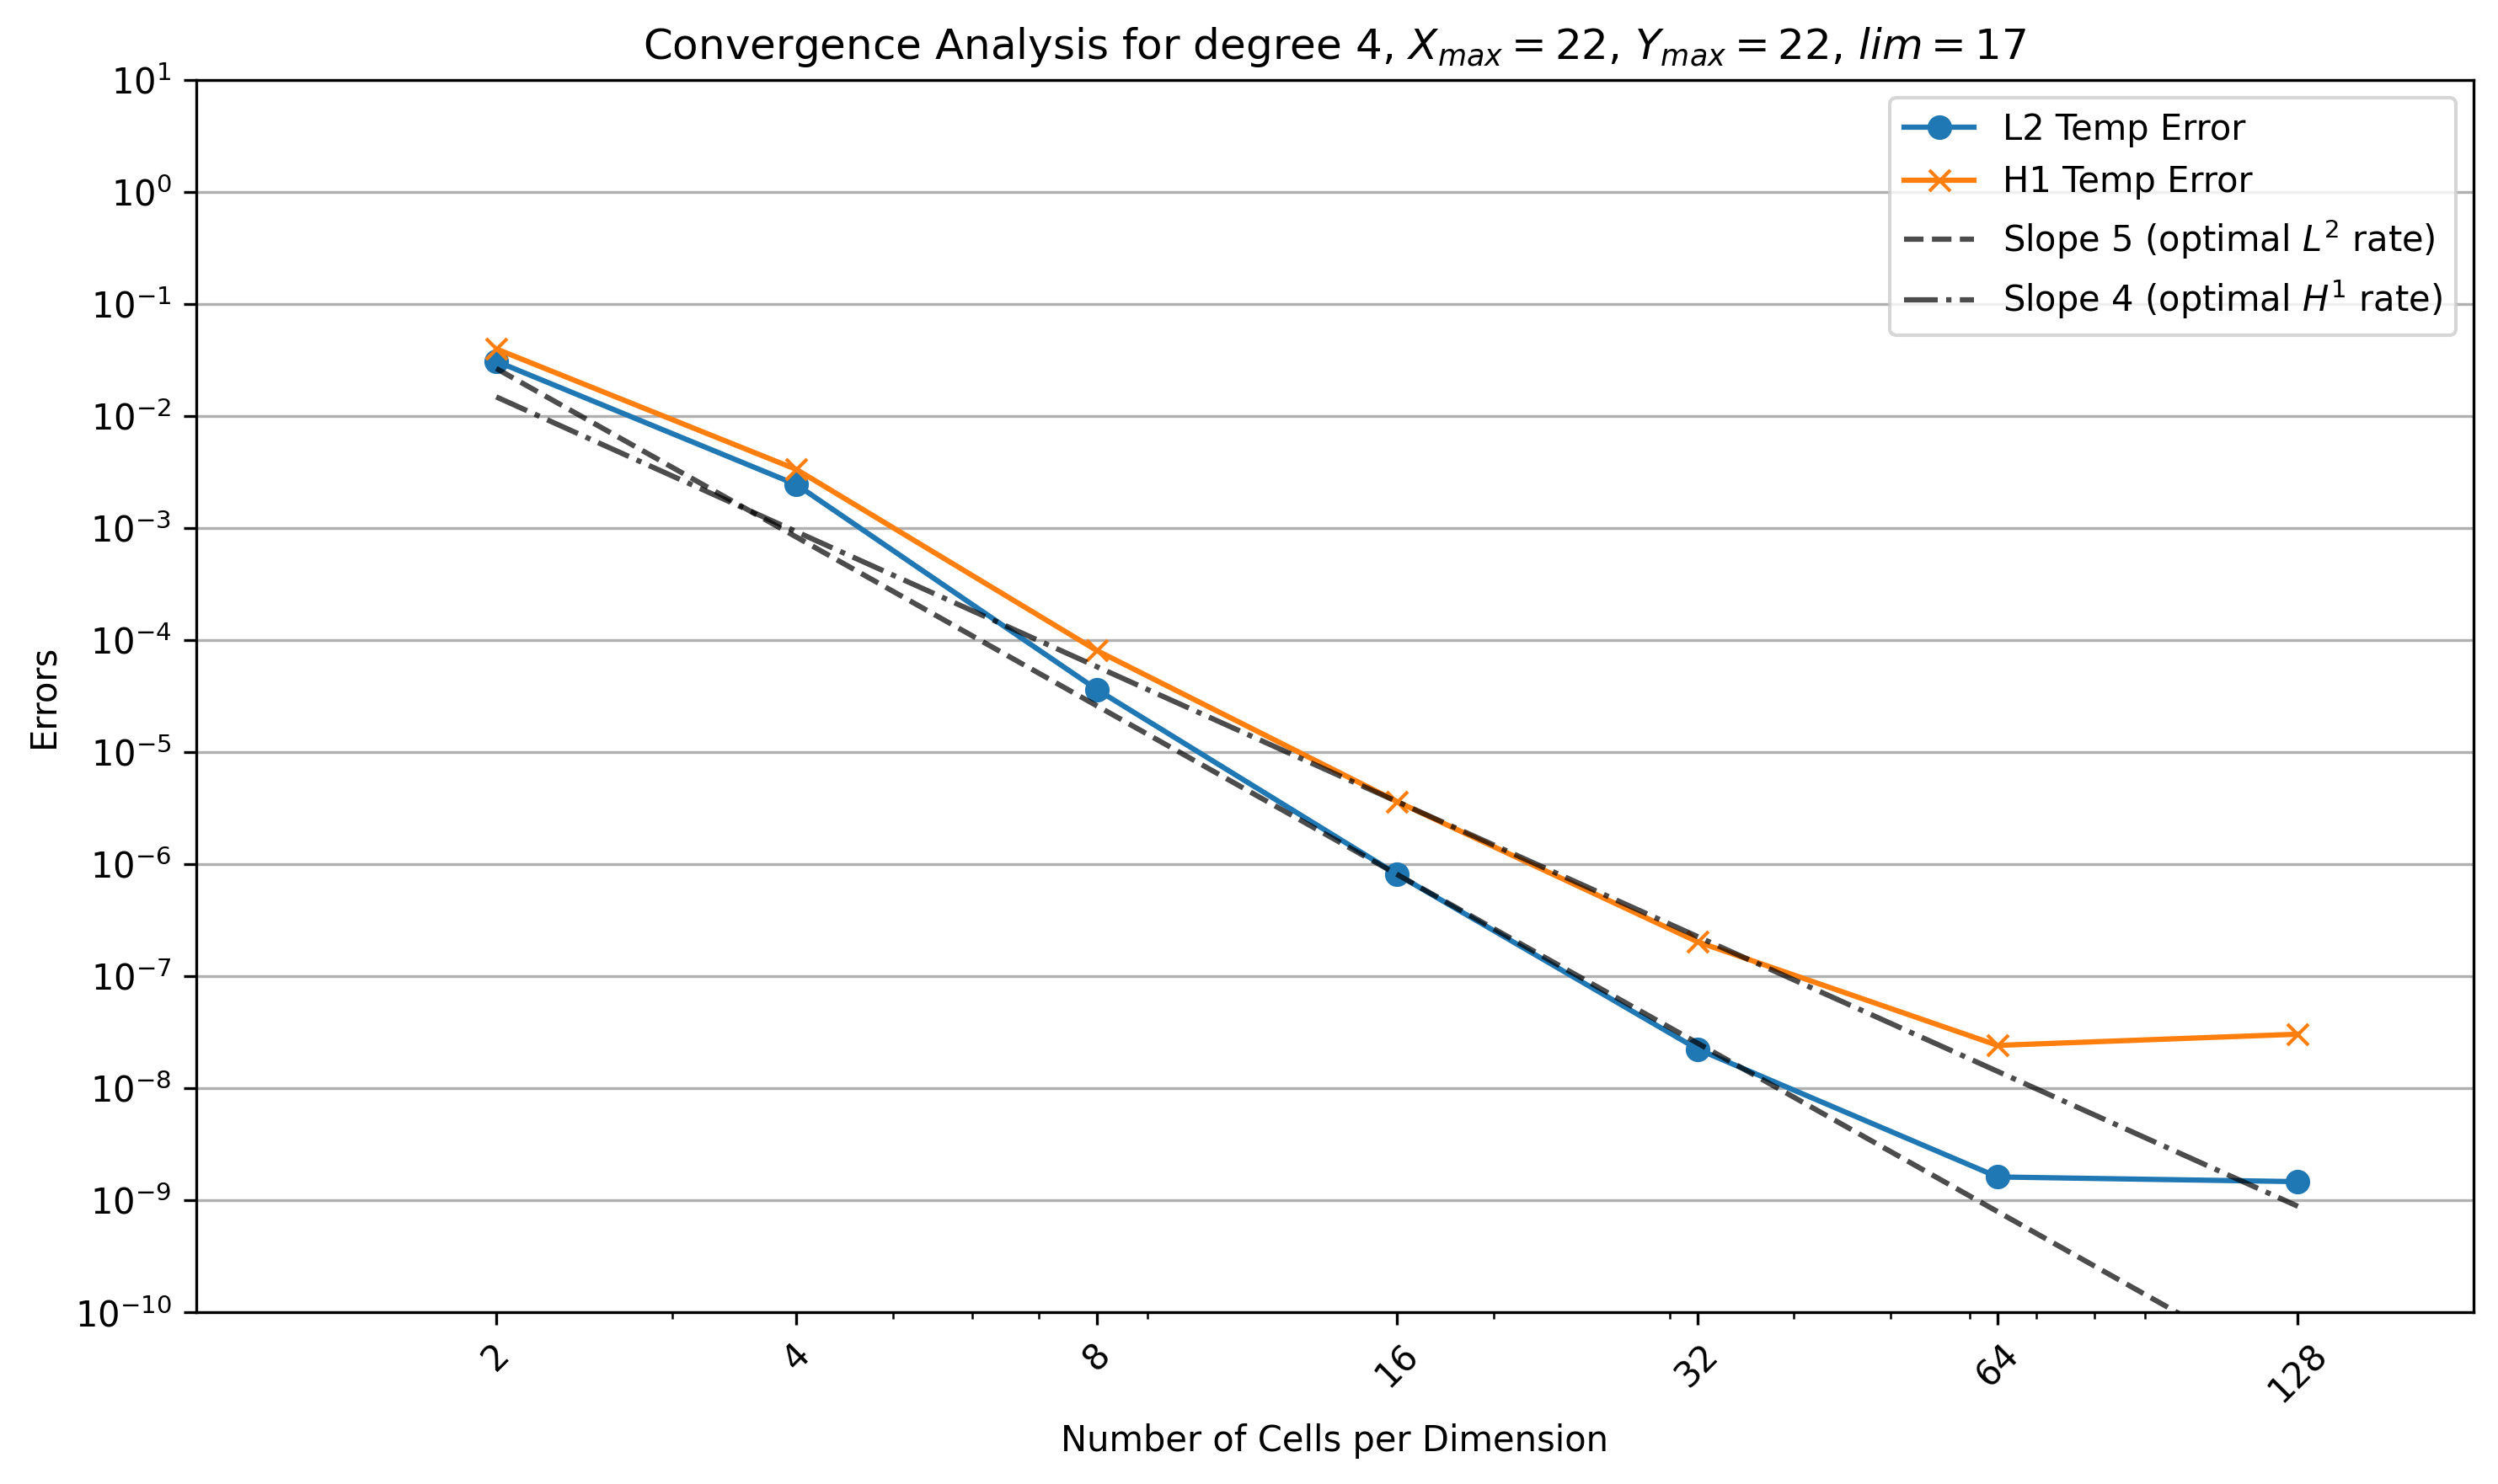
\includegraphics[width=\textwidth]{figures/figures_thermoelas_degree/Temp_X_max=22_Y_max=22_lim=17_d=4.png}
		\caption{Temperature field for degree 4 B-splines}
		\label{fig:temp_d4_lim_17}
	\end{subfigure}
	\begin{subfigure}[b]{0.49\textwidth}
		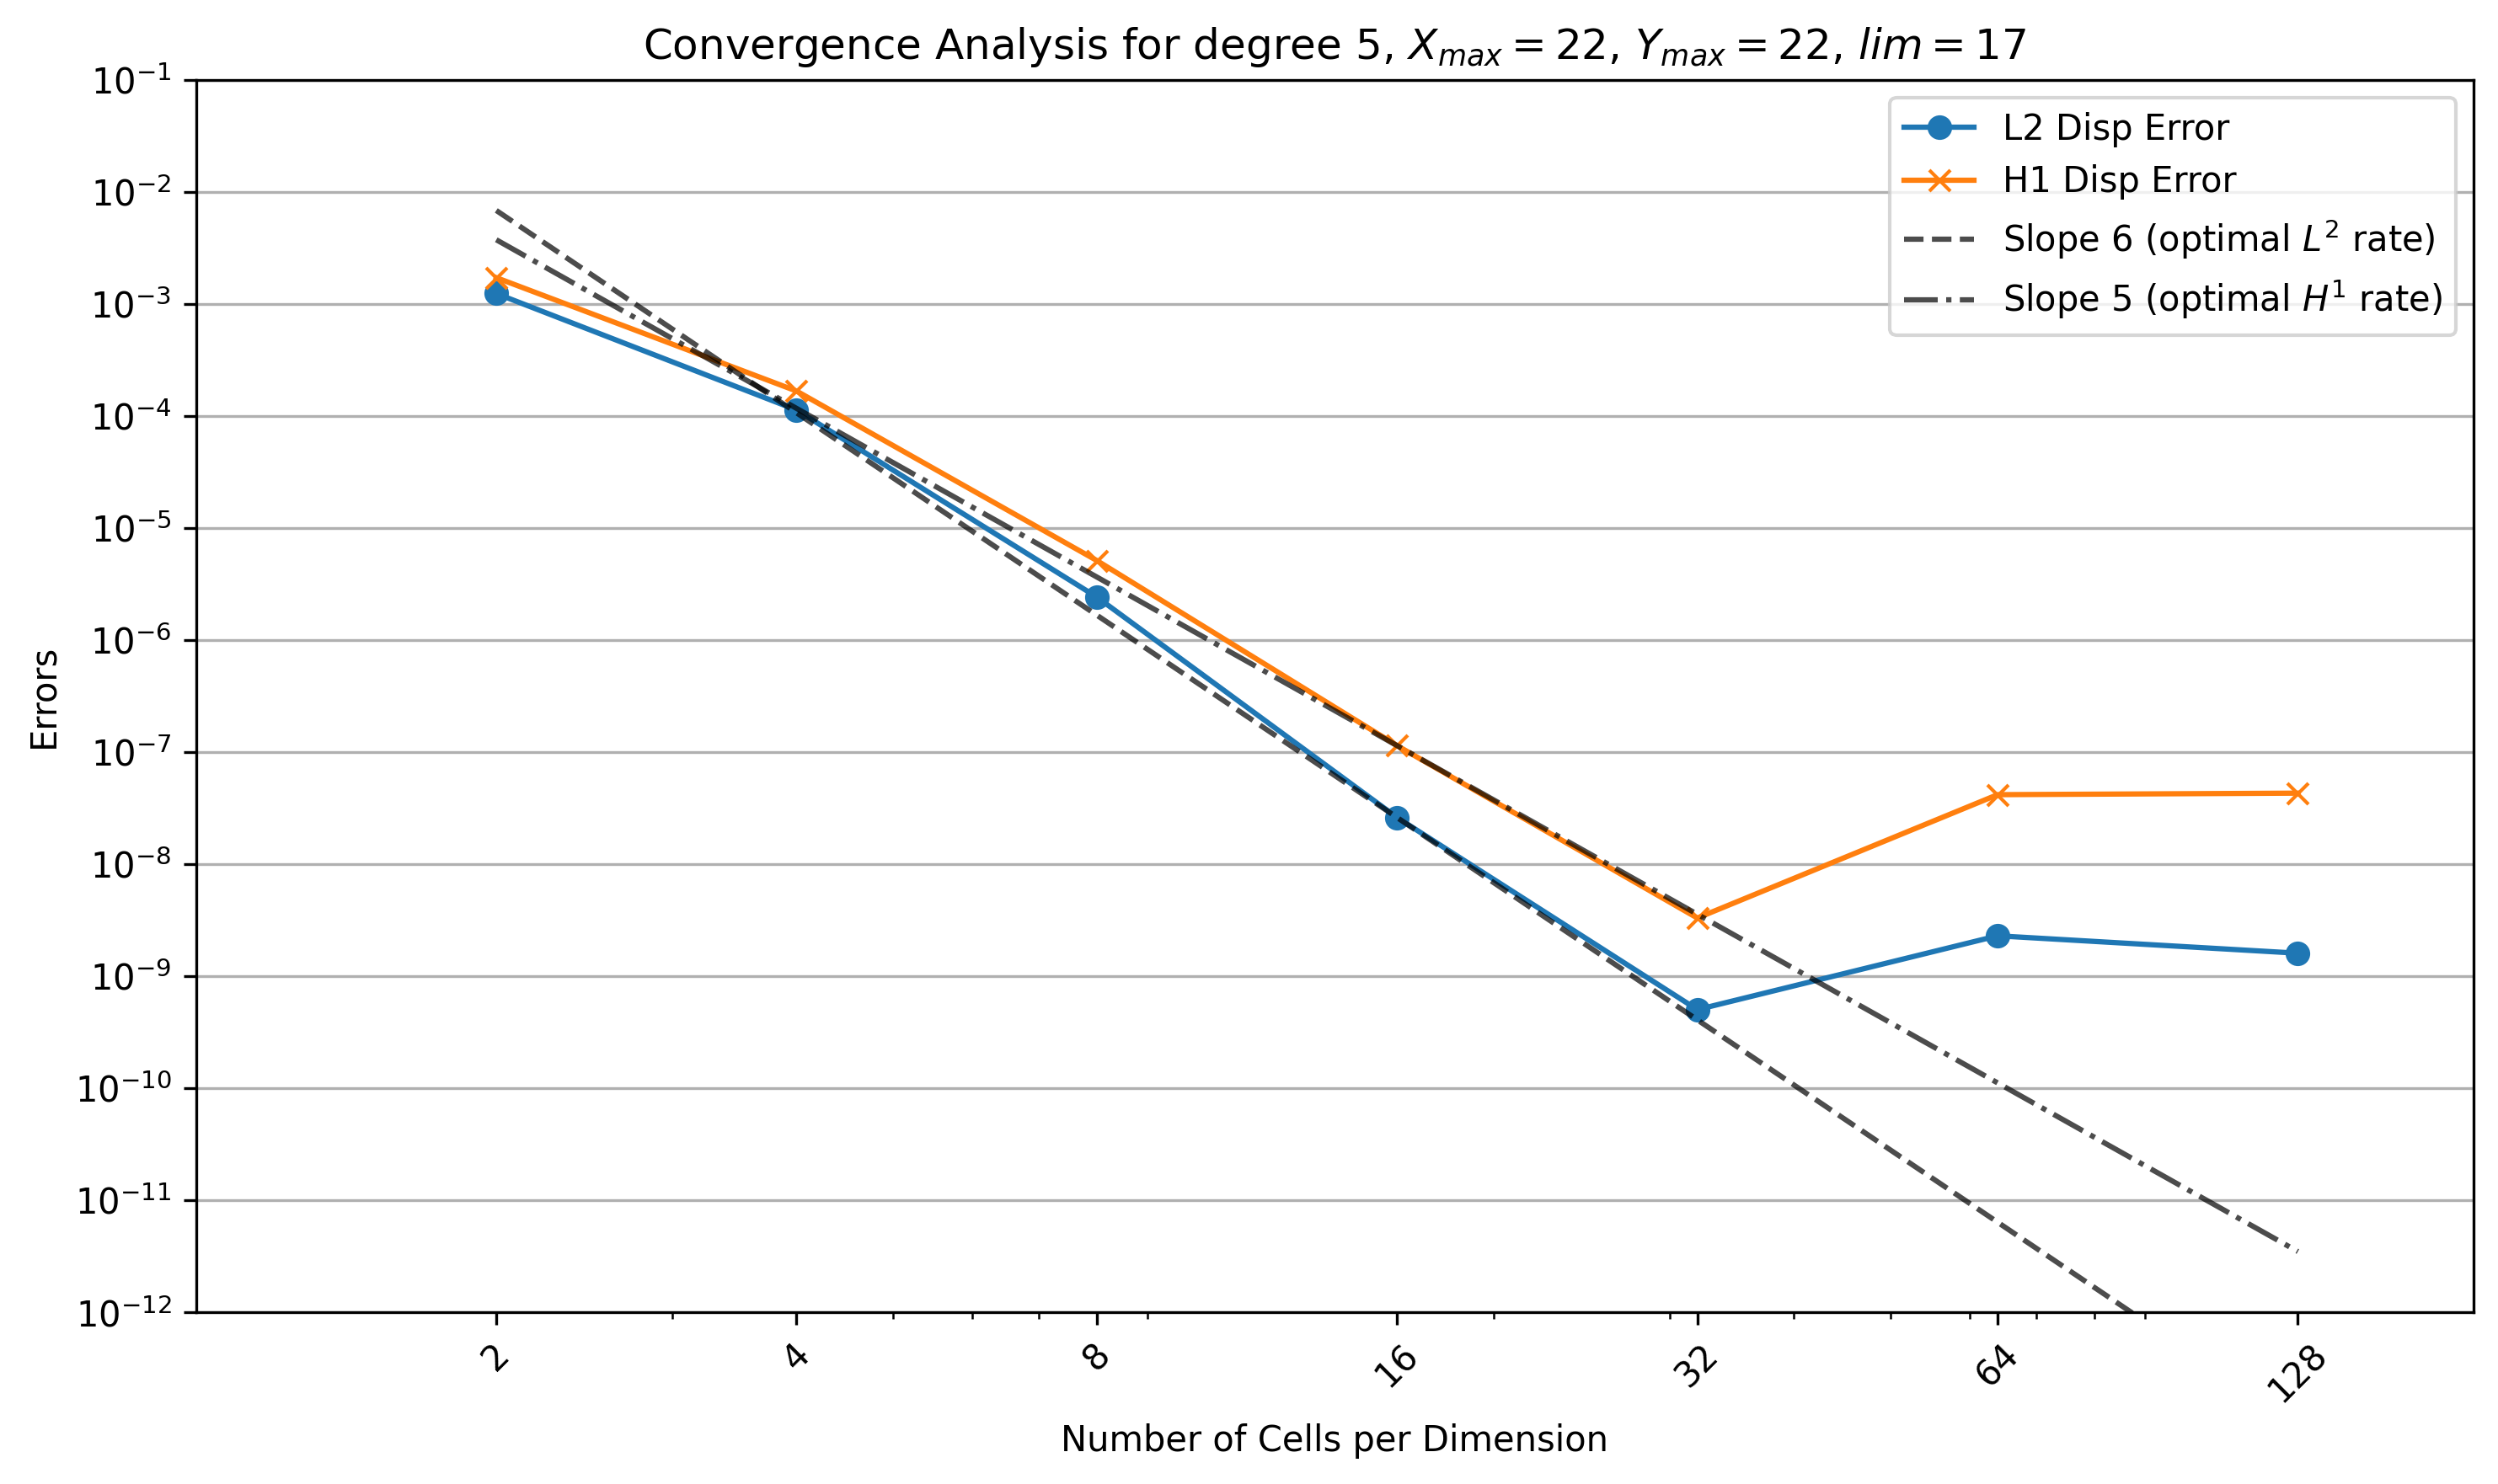
\includegraphics[width=\textwidth]{figures/figures_thermoelas_degree/Disp_X_max=22_Y_max=22_lim=17_d=5_disp.png}
		\caption{Displacement field for degree 5 B-splines}
		\label{fig:disp_d5_lim_17}
	\end{subfigure}
	\begin{subfigure}[b]{0.49\textwidth}
		\includegraphics[width=\textwidth]{figures/figures_thermoelas_degree/Temp_X_max=22_Y_max=22_lim=17_d=5.png}
		\caption{Temperature field for degree 5 B-splines}
		\label{fig:temp_d5_lim_17}
	\end{subfigure}
	\caption{Error plots of thermoelasticity with different degree B-splines using custom grid discretization with $\text{lim} = 17$}
\end{figure}

From the results presented in the previous figures, we can observe that the error curves validate the theoretical estimates established in equation \eqref{eq:approximation-estimates}. The convergence behavior follows the expected order for both the temperature and displacement fields across all tested degrees of B-splines. The numerical solution demonstrates optimal convergence rates consistent with the theoretical predictions for smooth solutions.

However, we can identify the plateau phenomenon when the error reaches certain threshold values, specifically around $10^{-9}$ for the $L^2$ norm and between $10^{-7}$ and $10^{-8}$ for the $H^1$ norm. This behavior mirrors exactly what was observed in Chapter \ref{chap:linear_elasticity}, suggesting that the underlying causes remain the same. The plateau effect is primarily attributed to the ill-conditioning of the system matrix, which becomes more pronounced as the mesh is refined and the degree of B-splines increases.

The error magnitudes are nearly identical for both the displacement and temperature fields. This similarity can be explained by the structure of our manufactured solutions: the exact temperature field $T_e$ is identical to the second component of the displacement field $\vec{u}_e$, while the first component of the displacement field is zero and $T_e$ appears in the source term when the displacement problem is solved. This deliberate choice in our test case creates a natural correspondence between the two fields, resulting in comparable approximation errors for both problems.

The successful implementation of the custom grid discretization feature has proven essential for handling the thermoelasticity problem with material property discontinuities at $y = 17$. This enhancement to \texttt{PSYDAC} enables accurate simulations in scenarios where material interfaces do not align with uniform grid boundaries, which is crucial for realistic engineering applications involving composite materials. It could be possible to use another main functionality of \texttt{PSYDAC}: resolution on a multipatch domain. This approach will be tackled in the next section. 

\section{Initial problem - Resolution on a multipatch domain}

In this section, we will consider the initial problem described in figure \ref{fig:geometry_thermoelasticity}. To model this medium and simulate the thermoelastic behavior, we will use the multipatch framework provided by \texttt{PSYDAC}.

\subsection{Quick overview of the multipatch framework}
\textit{This section presents a quick overview of the multipatch framework in \texttt{PSYDAC}. For a more detailed description of the multipatch framework, please refer t \cite{guclu_psydac_2022} and \cite{Guclu2023}} \\

The multipatch framework in \texttt{PSYDAC} allows for the simulation of problems defined on non-conforming grids, which is particularly useful for complex geometries and material interfaces. This framework enables the coupling of different patches, each potentially using different discretization strategies of mapping.

In \texttt{Psydac}, the \emph{multipatch framework} is designed to represent complex physical domains by decomposing them into a collection of simpler \emph{patches}. Each patch is the image of a logical domain (typically $[0,1]^d$) under a smooth mapping $F_k$. This approach allows the exact representation of curved geometries while maintaining a structured, tensor-product B-spline discretization within each patch.

Mathematically, each patch $\Omega_k$ supports a local finite element space $V_h^\ell(\Omega_k)$, built from tensor-product B-splines or NURBS of chosen degree and regularity. These local spaces form a discrete de Rham sequence
\[
V_h^0(\Omega_k) \xrightarrow{\nabla} V_h^1(\Omega_k) \xrightarrow{\nabla \times} V_h^2(\Omega_k) \xrightarrow{\nabla \cdot} V_h^3(\Omega_k),
\]
ensuring that key identities such as $\nabla \times (\nabla \varphi) = 0$ and $\nabla \cdot (\nabla \times \mathbf{u}) = 0$ hold at the discrete level.

The domain $\Omega$ is the union $\Omega = \bigcup_{k=1}^K \Omega_k$, and \texttt{Psydac} constructs the \emph{broken space}
\[
V_h^\ell := \left\{ v \in L^2(\Omega) \; \middle| \; v|_{\Omega_k} \in V_h^\ell(\Omega_k) \right\},
\]
which does not enforce conformity across patch interfaces. This choice yields block-diagonal mass matrices (one block per patch), enabling local $L^2$ projections and efficient parallelization. To recover the necessary continuity when required, \texttt{Psydac} applies \emph{conforming projection operators} $P_h^\ell$ that average interface degrees of freedom, defining discrete operators
\[
d_h^\ell = d^\ell \, P_h^\ell,
\]
where $d^\ell$ is the continuous differential operator. This guarantees the \emph{commuting diagram property} of Finite Element Exterior Calculus (FEEC), thus preserving stability, exactness of sequences, and the structure of discrete Hodge--Helmholtz decompositions.

This multipatch combined with the broken-FEEC approach provides:
\begin{enumerate}
	\item \textbf{Geometric flexibility}: each patch can have its own parametrization, allowing the exact modeling of complex CAD geometries;
	\item \textbf{Computational locality}: operators and projections involve only neighboring patches, enhancing scalability for large-scale parallel simulations.
\end{enumerate}

For example, \texttt{PSYDAC} can reproduce a Pretzel geometry by defining multiple patches that conform to the intricate shape of the object. Each patch can be individually parameterized to capture the local geometry accurately, while the multipatch framework ensures that the overall simulation remains consistent and stable. Then, it's possible to solve Poisson's equation or Time-dependent Maxwell equations on a Pretzel geometry.
\newpage
\begin{figure}[!h]
	\centering
	\includegraphics[width=1\textwidth]{figures/maxwell_pretzel.png}
	\caption{Time harmonic Maxwell's equation on a pretzel domain with inhomogeneous essential boundary conditions. Multi-patch domain (left), numerical amplitude $|u_h|$ (center) and amplitude error $|u_{ex}| - |u_h|$ (right) obtained with polynomial degree $p = 3$ and $N = 1$ from \cite{guclu_psydac_2022}}
\end{figure}

In this context, the multipatch framework is particularly advantageous for handling the thermoelasticity problem with this unusual geometry. 

\subsection{A simple multipatch: square hole}

To get familiar with the multipatch framework, we start with a simple example: a square domain with a square hole in the center. This geometry can be easily represented using a multipatch approach with 8 square patches. Actually, the domain can be described with fewer patches but to define correctly the boundary conditions, we need to define the patches in a way that allows us to apply the Dirichlet boundary conditions on the entire boundary of the domain.

\begin{figure}[!h]
	\centering
	\includegraphics[width=0.5\textwidth]{figures/square_hole.png}
	\caption{Multipatch representation of a square domain with a square hole in the center.}
\end{figure}

In this case, the hole is represented by a square $[5,17] \times [3,15]$ and is surrounded by 8 patches. Each patch is obtained by applying a transformation to the reference square $[0,1]^2$. The patches are defined as follows: $\forall (\hat x, \hat y) \in [0,1]^2$,
\begin{itemize}
	\item Patch 1: $\Omega_1 := [0,5] \times [0,3]$ with $F_1(\hat x, \hat y) = (5\hat x, 3\hat y)$
	\item Patch 2: $\Omega_2 := [5,17] \times [0,3]$ with $F_2(\hat x, \hat y) = (12\hat x + 5, 3\hat y)$
	\item Patch 3: $\Omega_3 := [17,22] \times [0,3]$ with $F_3(\hat x, \hat y) = (5\hat x + 17, 3\hat y)$
	\item Patch 4: $\Omega_4 := [0,5] \times [3,15]$ with $F_4(\hat x, \hat y) = (5\hat x, 12\hat y + 3)$
	\item Patch 5: $\Omega_5 := [17,22] \times [3,15]$ with $F_5(\hat x, \hat y) = (5\hat x + 17, 12\hat y + 3)$
	\item Patch 6: $\Omega_6 := [0,5] \times [15,22]$ with $F_6(\hat x, \hat y) = (5\hat x, 7\hat y + 15)$
	\item Patch 7: $\Omega_7 := [5,17] \times [15,22]$ with $F_7(\hat x, \hat y) = (12\hat x + 5, 7\hat y + 15)$
	\item Patch 8: $\Omega_8 := [17,22] \times [15,22]$ with $F_8(\hat x, \hat y) = (5\hat x + 17, 7\hat y + 15)$
\end{itemize}

The physical domain is then defined as the union of these patches: $$\Omega = \bigcup_{i=1}^8 \Omega_i = ([0,22] \times [0,22]) \setminus ([5,17] \times [3,15])$$.
The code to define this multipatch domain in \texttt{PSYDAC} is given in Section \ref{sec:multipatch_code}.

The use of a multipatch domain needs to ensure that the patches are properly aligned and that the transformations between them are smooth. Moreover, bilinear forms must be defined consistently across patch boundaries to ensure the stability and accuracy of the numerical methods employed. 
To do so, we call $\Sigma_{ij}$ the interface between patches $\Omega_i$ and $\Omega_j$, such that $\Sigma_{ij} = \partial \Omega_i \cap \partial \Omega_j$.

Then, bilinear forms are penalized across the interfaces to ensure continuity and stability: this is called Nitsche's method. 
This method consists of adding a penalty term to the bilinear forms that involves the traces of the functions on the interface $\Sigma_{ij}$, a symmetrization term and a penalty term that ensures the continuity of the traces across the interface \cite{fritz_comparison_2004} \cite{Hansbo2003}.
Consequently, the bilinear forms are redefined as follows:

\begin{align*}
a(\vec u,\vec v) &= a_\Omega(\vec u,\vec v) + \sum_{i,j} a_{ij}(\vec u,\vec v) \\
b(T,\Theta) &= b_\Omega(T,\Theta) + \sum_{i,j} b_{ij}(T,\Theta)
\end{align*}
With: 
\begin{equation*}
	\begin{aligned}
	& a_\Omega : \left\{
		\begin{aligned}
			& \boldsymbol{H}^1_{\vec 0,D}(\Omega) \times \boldsymbol{H}^1_{\vec 0,D}(\Omega) \longrightarrow \mtr \\
			& (\vec u, \vec v) \mapsto \int_{\Omega} \Big( \lambda(y) (\div \vec u) (\div \vec v) + 2\mu(y) \boldsymbol{\varepsilon}(\vec u) : \boldsymbol{\varepsilon}(\vec v) \Big) \, d\Omega 
		\end{aligned}
	\right. \\
	& a_{ij} : \left\{
		\begin{aligned}
			& \boldsymbol{H}^1_{\vec 0,D}(\Omega) \longrightarrow \mtr \\ 
			& (\vec u, \vec v) \mapsto \int_{\Sigma_{ij}} - \{\boldsymbol{\sigma}(\vec u) \cdot \vec n\} \cdot \left[\left[ \vec v \right]\right] - \{\boldsymbol{\sigma}(\vec v) \cdot \vec n\} \cdot \left[\left[ \vec u \right]\right] + \gamma_u \frac{\{2 \mu + \lambda\}}{h} \left[\left[ \vec u \right]\right] \cdot \left[\left[ \vec v \right]\right] \, d\Gamma
		\end{aligned}
	\right.\\
	& b_\Omega : \left\{
		\begin{aligned}
			& H^1_{0,\text{temp}}(\Omega) \times H^1_{0,\text{temp}}(\Omega) \longrightarrow \mtr \\
			& (T, \theta) \mapsto \int_{\Omega} \kappa(y) \grad T \cdot \grad \theta \, d\Omega 
		\end{aligned}
	\right. \\
	& b_{ij} : \left\{
		\begin{aligned}
			& H^1_{0,\text{temp}}(\Omega) \times H^1_{0,\text{temp}}(\Omega) \longrightarrow \mtr \\
			& (T, \theta) \mapsto \int_{\Sigma_{ij}} - \{ \kappa(y) \grad T \cdot \vec n \} \left[\left[ \theta \right]\right] - \{ \kappa(y) \grad \theta \cdot \vec n \}  \left[\left[ T \right]\right] + \gamma_T \frac{\{ \kappa \}}{h} \left[\left[ T \right]\right]\left[\left[ \theta \right]\right] \, d\Gamma
		\end{aligned}
	\right. \\
	& \text{Where } \{ \cdot \} \text{ denotes the average across the interface } \Sigma_{ij}, \left[\left[\cdot\right]\right] \text{ denotes the jump and } \\
	& \gamma_u, \gamma_T > 0 \text{ are penalty parameters.} 
	\end{aligned}
\end{equation*}

% I have also added Dirichlet weak conditions for the displacement on the boundary of the domain to ensure that the solution satisfies the desired behavior on the boundary. This is characterized by an additional bilinear and linear form for the displacement problem:
% \begin{equation*}
% 	\begin{aligned}
% 	& a_{\text{weak Dirichlet}} : \left\{
% 		\begin{aligned}
% 			& \boldsymbol{H}^1(\Omega) \times \boldsymbol{H}^1(\Omega) \longrightarrow \mtr \\
% 			& (\vec u, \vec v) \mapsto \int_{\partial\Omega_D} - \boldsymbol{\sigma}(\vec u) \cdot \vec n \cdot \vec v - \boldsymbol{\sigma}(\vec v) \cdot \vec n \cdot \vec u + \gamma_u \frac{2\mu + \lambda}{h} \vec u \cdot \vec v \, dS
% 		\end{aligned}
% 	\right. \\
% 	& l_{U,\text{weak Dirichlet}} : \left\{
% 		\begin{aligned}
% 			& \boldsymbol{H}^1(\Omega) \longrightarrow \mtr \\
% 						& \vec v \mapsto \int_{\partial\Omega_D} - \boldsymbol{\sigma}(\vec v) \cdot \vec n \cdot \vec u_D + \gamma_u \frac{2\mu + \lambda}{h} \vec u_D \cdot \vec v \, dS
% 		\end{aligned}
% 	\right.
% 	\end{aligned}
% \end{equation*}

With these modifications, the complete weak formulation for the thermoelasticity problem on the multipatch domain becomes:
\begin{tcolorbox}
Find $(T, \vec u) \in H^1(\Omega) \times \boldsymbol{H}^1(\Omega)$ such that for all test functions $(\theta, \vec v) \in H^1(\Omega) \times \boldsymbol{H}^1(\Omega)$:
\begin{equation}
	\left\{
	\begin{aligned}
		b_{\Omega}(T, \theta) + \sum_{i \neq j} b_{ij}(T, \theta) &= l_{T}(\theta) \\
		a_{\Omega}(\vec u, \vec v) + \sum_{i \neq j} a_{ij}(\vec u, \vec v) &= l_{U}(\vec v)
	\end{aligned}
	\right.
\end{equation}
\end{tcolorbox}

The penalty parameters $\gamma_u$ and $\gamma_T$ must be chosen sufficiently large to ensure stability while maintaining accuracy. Typically, values in the range $[10, 100]$ work well in practice, though the optimal choice may depend on the specific problem parameters and mesh size.

This multipatch formulation with Nitsche's method allows for flexible handling of complex geometries while maintaining the stability and convergence properties of the underlying finite element discretization. The approach is particularly well-suited for problems involving material interfaces, complex boundaries, or domains that cannot be easily represented by a single structured mesh.

To test the convergence of the simulation on the multipatch domain, we use the same exact functions $T_e$ and $\vec{u}_e$ as defined in the previous section:

$$
T_e = \sin\left(\frac{\pi x}{22}\right) \sin\left(\frac{\pi y}{22}\right) \qquad \vec u_e = \begin{pmatrix}
	0 \\
	\sin\left(\frac{\pi x}{22}\right) \sin\left(\frac{\pi y}{22}\right) 
\end{pmatrix}
$$

For the multipatch convergence test, we impose Dirichlet boundary conditions on all boundaries of the global domain $\partial\Omega$. This means that both the temperature and displacement fields are prescribed on the entire outer boundary of the domain (excluding the hole). The boundary conditions are therefore:

\begin{align}
	T &= T_e \quad &&\text{on } \partial\Omega \\
	\vec u &= \vec u_e \quad &&\text{on } \partial\Omega
\end{align}

With these boundary conditions, the corresponding source terms are computed as:
\begin{equation*}
	\begin{aligned}
	& Q = - \div(\kappa(y) \grad T_e), \\
	& \vec f = -\div \boldsymbol{\sigma}(\vec u_e)
	\end{aligned}
\end{equation*}

This test configuration allows us to verify that the multipatch implementation correctly handles the coupling between patches while maintaining the expected convergence rates for both the temperature and displacement fields.

\begin{figure}[!h]
	\centering
	\begin{subfigure}[b]{\textwidth}
		\centering
		\includegraphics[width=0.9\textwidth]{figures/figures_multipatch/temperature.png}
		\caption{Temperature field: $T_e$ (left) - $T_h$ (center) - Error (right)}
	\end{subfigure}
\end{figure}

Unfortunately, my implementation of the multipatch method is not yet complete. The simulation is running, but the displacement problem doesn't converge as expected. The displacement numerical solution seems to have some continuity problems between interfaces, while the thermal simulation seems to be working correctly.

\begin{figure}  \ContinuedFloat
	\centering
	\begin{subfigure}[b]{\textwidth}
		\centering
		\includegraphics[width=0.9\textwidth]{figures/figures_multipatch/ux.png}
		\caption{Displacement field on x-axis: $u_{e,x}$ (left) - $u_{h,x}$ (center) - Error (right)}
		\label{fig:ux_multipatch}
	\end{subfigure}
	\begin{subfigure}[b]{\textwidth}
		\centering
		\includegraphics[width=0.9\textwidth]{figures/figures_multipatch/uy.png}
		\caption{Displacement field on y-axis: $u_{e,y}$ (left) - $u_{h,y}$ (center) - Error (right)}
		\label{fig:uy_multipatch}
	\end{subfigure}
	\caption{Simulation plots on a multipatch domain with $n_{cells} = 64$ per direction and domain with degree $p = 2$ B-Splines}
\end{figure}

As we can see in figures \ref{fig:ux_multipatch} and \ref{fig:uy_multipatch}, the displacement field on the x-axis is not continuous across the interfaces, which leads to non-convergence of the numerical solution. The error is not decreasing as expected, and the solution is not smooth across the interfaces. This issue is likely due to the Nitsche's method implementation or the way the bilinear forms are defined across the interfaces. Even by changing the values of constant $\gamma_u$ to different values, the solution is not converging as expected...

\begin{figure}[!h]
	\centering
	\begin{subfigure}[b]{0.49\textwidth}
		\centering
		\includegraphics[width=\textwidth]{figures/figures_multipatch/Temp_multipatch.png}
		\caption{Error on the temperature field}
		\label{fig:error_temp_multipatch}
	\end{subfigure}
	\begin{subfigure}[b]{0.49\textwidth}
		\centering
		\includegraphics[width=\textwidth]{figures/figures_multipatch/Disp_multipatch.png}
		\caption{Error on the displacement field}
		\label{fig:error_disp_multipatch}
	\end{subfigure}
	\caption{Error plots on a multipatch domain with degree $p = 2$ B-Splines}
\end{figure}

Looking at the error plots across the number of cells, the error on the displacement field seems to be constant, while the error on the temperature field is decreasing. To a certain extent, the error on temperature is decreasing as expected...
One can suppose that the Nitsche's method is not enforcing the continuity of the displacement field across the interfaces properly, leading to the observed constant error. However, this problem needs further investigation and potentially a different approach to ensure the continuity of the displacement field across the interfaces.

\section{Conclusion}

This chapter has explored the application of thermoelasticity problems within the \texttt{PSYDAC} framework, demonstrating the library's capability to handle coupled thermo-mechanical systems with varying material properties. The study encompassed two main configurations: a simplified square domain and a more complex geometry with a hole requiring multipatch treatment. \\

The simplified problem provided valuable insights into the behavior of coupled thermoelasticity systems under thermal and mechanical loads. The theoretical foundation, based on the stationary coupling between heat conduction and linear elasticity equations, was successfully implemented and validated using manufactured solutions. The decoupled approach, where temperature is solved first and then used as a source term in the mechanical problem, proved effective for the material parameters considered. \\

A significant achievement of this work was the development and implementation of custom grid discretization capabilities in \texttt{PSYDAC}. The custom grid feature enables practitioners to strategically place mesh boundaries at material interfaces, ensuring that the B-spline basis functions properly capture the discontinuous nature of material properties. This capability is essential for realistic engineering applications involving composite materials, layered structures, or any scenario where material properties vary abruptly within the computational domain. \\

The exploration of multipatch methods for complex geometries represents an ambitious extension of the work, though it revealed implementation challenges that require further development. While the thermal problem showed encouraging results on the multipatch domain, the displacement field exhibited continuity issues across patch interfaces. This suggests that the Nitsche method implementation for the elasticity equations needs refinement to properly enforce interface conditions for vector-valued problems. \\

The difficulties encountered with the multipatch approach highlight the complexity of ensuring proper coupling between patches for systems of PDEs.
Despite these challenges, the thermoelasticity work has significantly expanded \texttt{PSYDAC}'s application domain. The custom grid discretization feature alone represents a valuable contribution that enables the library to handle realistic material configurations common in engineering practice. The insights gained from the coupling of thermal and mechanical fields provide a foundation for future developments in multiphysics simulations. \\

\chapter{Conclusion}
\vspace{-1cm}
This research internship at the Max Planck Institute for Plasma Physics has been a great experience that successfully achieved its primary objectives while providing invaluable insights into the computational mechanics domain. The work has demonstrated that \texttt{PSYDAC}, originally designed for plasma physics applications, can be effectively extended to solve solid mechanics problems, particularly linear elasticity and thermoelasticity equations.


\paragraph{\underline{Scientific Achievements:}}
This internship extended \texttt{PSYDAC} from plasma physics to solid mechanics, implementing two formulations for linear elasticity, developing custom grid discretization for thermoelasticity problems with material discontinuities, and exploring multipatch methods for complex geometries. The work validated theoretical convergence rates, identified volumetric locking limitations in incompressible materials, and contributed essential capabilities for handling composite materials and coupled multiphysics simulations within the IGA framework.

\paragraph{\underline{Methodological Insights and Personal Growth:}}

This internship provided me with a profound understanding of the research methodology, particularly the systematic decomposition of complex problems into manageable steps. Working with \texttt{PSYDAC} on the Raven supercomputer taught me that effective research progress comes through patient iteration and careful validation. The experience enhanced my computational skills while developing a holistic perspective on the interplay between theoretical foundations, practical implementation constraints, and high-performance computing resource management, insights that will prove invaluable for future scientific endeavors. I've also come to understand the high-performance tools at my disposal and how to leverage them effectively in my research to avoid excessive resource consumption.

\paragraph{\underline{Collaborative Outcomes and Future Prospects:}}

This internship will contribute directly to a presentation at the International Conference on Isogeometric Analysis (IGA 2025) in the Netherlands in September 2025. Moreover, my work will be part of a collaborative publication with Dr. Yaman Güçlü.

\paragraph{\underline{Personal Reflection:}}
Beyond the technical achievements, this internship has been profoundly enriching on a personal level. Working within an international research environment at IPP exposed me to diverse perspectives and collaborative approaches that broadened my understanding of scientific research culture. The experience of presenting complex technical concepts and contributing to open-source projects enhanced both my technical skills and professional confidence.

\begin{figure}[!t]
	\centering
	\includegraphics[width=1\textwidth]{figures/Timeline.jpg}
	\caption{Internship Timeline}
	\label{fig:internship_timeline}
\end{figure}

\newpage
\vspace{-1cm}
\printbibliography[heading=bibnumbered]

\newpage
\chapter{Appendices}
\section{Simulation code for linear elasticity with Dirichlet Homogeneous Boundary Conditions}
\label{sec:lin_elas_dirichlet}

\begin{lstlisting}[caption=Simulation code for the linear elasticity problem with Dirichlet boundary conditions.]
from mpi4py import MPI
from sympde.expr import BilinearForm, LinearForm, integral
from sympde.expr     import find, EssentialBC, Norm, SemiNorm
from sympde.topology import VectorFunctionSpace, Cube, element_of, Union, NormalVector
from sympde.calculus import grad, inner, div, Transpose
from sympde.core import Constant
from sympde.core import Matrix

from sympy import Identity, Tuple, sin, pi, cos, diff

import matplotlib.pyplot as plt
import numpy as np
import time

from psydac.api.settings import PSYDAC_BACKENDS


from psydac.api.discretization import discretize
import os
import numpy as np
import matplotlib.pyplot as plt

def run_lin_elas_non_mixed(ncells, degree, lambda_val, mu_val, comm=None, backend=None, solver_tol=1e-8):

    #+++++++++++++++++++++++++++++++
    # 1. Abstract model
    #+++++++++++++++++++++++++++++++

    domain = Cube()

    timing   = {}
    t0 = time.time()

    domain = Cube()

    nn = NormalVector(domain.boundary)


    lambda_ = Constant('lambda_', is_real=True, real=True)
    mu   = Constant('mu',   is_real=True, real=True)

    # Symbolic symmetric strain tensor
    def epsilon_symb(w):
        return 0.5 * (grad(w) + Transpose(grad(w)))

    # Symbolic stress tensor
    def sigma_symb(w):
        return lambda_ * div(w) * Identity(3) + 2 * mu * epsilon_symb(w)

    # Define the symmetric strain tensor (for to compute the source term)
    def epsilon(w): 
        grad_w = Matrix([
            [diff(w[0], x), diff(w[0], y), diff(w[0], z)],
            [diff(w[1], x), diff(w[1], y), diff(w[1], z)],
            [diff(w[2], x), diff(w[2], y), diff(w[2], z)]
        ])
        return 0.5 * (grad_w + grad_w.T)

    # Define the stress tensor (to compute the source terms)
    def sigma(w):
        eps = epsilon(w)
        div_w = diff(w[0], x) + diff(w[1], y) + diff(w[2], z)
        C_eps = lambda_ * div_w * Identity(3) + 2 * mu * eps
        return C_eps

    V = VectorFunctionSpace('V', domain)

    x,y,z = domain.coordinates

    u,v = [element_of(V, name=i) for i in ['u', 'v']]

    # Bilinear form
    a = BilinearForm((u,v), integral(domain , inner(sigma_symb(u), epsilon_symb(v))))


    # Exact solution
    ue1 = 0
    ue2 = 0
    ue3 = sin(pi*x)*sin(pi*y)*sin(pi*z)
    ue = Tuple(ue1, ue2, ue3)

    # Second member
    sigma_ue = sigma(ue)
    f1 = diff(sigma_ue[0, 0], x) + diff(sigma_ue[0, 1], y) + diff(sigma_ue[0, 2], z)
    f2 = diff(sigma_ue[1, 0], x) + diff(sigma_ue[1, 1], y) + diff(sigma_ue[1, 2], z)
    f3 = diff(sigma_ue[2, 0], x) + diff(sigma_ue[2, 1], y) + diff(sigma_ue[2, 2], z)
    f = Tuple(-f1, -f2, -f3)

    # Linear forms
    l = LinearForm(v, integral(domain, inner(f, v)))

    # Dirichlet boundary conditions
    bc = [EssentialBC(u, 0, domain.boundary)]

    # Variational problem
    equation = find(u, forall=v, lhs=a(u, v), rhs=l(v), bc=bc)

    error = Matrix([u[0]-ue[0], u[1]-ue[1], u[2]-ue[2]])

    l2norm = Norm(error, domain, kind='l2')
    h1norm = Norm(error, domain, kind='h1')
    h1_seminorm = SemiNorm(error, domain, kind='h1')

    t1 = time.time()
    timing["Abstract model"] = t1-t0

    #+++++++++++++++++++++++++++++++
    # 2. Discretization
    #+++++++++++++++++++++++++++++++

    t0 = time.time()
    domain_h = discretize(domain, ncells=ncells, comm=comm)
    Vh       = discretize(V, domain_h, degree=degree)

    equation_h = discretize(equation, domain_h, [Vh, Vh], backend=backend)

    l2norm_h = discretize(l2norm, domain_h, Vh, backend=backend)
    h1norm_h = discretize(h1norm, domain_h, Vh, backend=backend)
    h1_seminorm_h = discretize(h1_seminorm, domain_h, Vh, backend=backend)

    #+++++++++++++++++++++++++++++++
    # 3. Solver & Errors
    #+++++++++++++++++++++++++++++++

    equation_h.set_solver('gmres', info=True, tol=solver_tol)

    t1 = time.time()
    timing["Discretization"] = t1-t0

    comm.Barrier()
    t0       = time.time()
    uh, info = equation_h.solve(mu=mu_val, lambda_=lambda_val)
    t1       = time.time()
    timing['solution'] = t1-t0

    comm.Barrier()
    t0 = time.time()
    l2_error = l2norm_h.assemble(u=uh)
    h1_error = h1norm_h.assemble(u=uh)
    h1_seminorm_error = h1_seminorm_h.assemble(u=uh)
    t1       = time.time()

    timing['diagnostics'] = t1-t0
    timing["Abstract model"] = comm.reduce(timing["Abstract model"], op=MPI.MAX)
    timing["Discretization"] = comm.reduce(timing["Discretization"], op=MPI.MAX)
    timing['solution']       = comm.reduce(timing['solution'], op=MPI.MAX)
    timing['diagnostics']    = comm.reduce(timing['diagnostics'], op=MPI.MAX)

    return uh, info, timing, l2_error, h1_error, h1_seminorm_error
\end{lstlisting}


\section{Multipatch domain decomposition with PSYDAC}
\label{sec:multipatch_code}
\vspace{-0.5cm}
\begin{lstlisting}[caption=Multipatch domain decomposition with PSYDAC.]
from psydac.feec.multipatch.multipatch_domain_utilities import sympde_Domain_join
from sympde.topology import Square
from sympde.topology import IdentityMapping

def build_domain_hole(domain_name="domain"):
    OmegaLog1 = Square('OmegaLog1', bounds1=(0., 5), bounds2=(0., 3))
    mapping_1 = IdentityMapping('M1', 2)
    domain_1 = mapping_1(OmegaLog1)

    OmegaLog2 = Square('OmegaLog2', bounds1=(5, 17), bounds2=(0., 3))
    mapping_2 = IdentityMapping('M2', 2)
    domain_2 = mapping_2(OmegaLog2)

    OmegaLog3 = Square('OmegaLog3', bounds1=(17, 22), bounds2=(0., 3))
    mapping_3 = IdentityMapping('M3', 2)
    domain_3 = mapping_3(OmegaLog3)

    OmegaLog4 = Square('OmegaLog4', bounds1=(0, 5), bounds2=(3, 15))
    mapping_4 = IdentityMapping('M4', 2)
    domain_4 = mapping_4(OmegaLog4)

    OmegaLog6 = Square('OmegaLog6', bounds1=(17, 22), bounds2=(3, 15))
    mapping_6 = IdentityMapping('M6', 2)
    domain_6 = mapping_6(OmegaLog6)

    OmegaLog7 = Square('OmegaLog7', bounds1=(0, 5), bounds2=(15, 22))
    mapping_7 = IdentityMapping('M7', 2)
    domain_7 = mapping_7(OmegaLog7)

    OmegaLog8 = Square('OmegaLog8', bounds1=(5, 17), bounds2=(15, 22))
    mapping_8 = IdentityMapping('M8', 2)
    domain_8 = mapping_8(OmegaLog8)

    OmegaLog9 = Square('OmegaLog9', bounds1=(17, 22), bounds2=(15, 22))
    mapping_9 = IdentityMapping('M9', 2)
    domain_9 = mapping_9(OmegaLog9)
    
    # 7 8 9
    # 4 * 6
    # 1 2 3
    patches = [domain_1, domain_2, domain_3, domain_4, domain_6, domain_7, domain_8, domain_9]
    axis_0, axis_1 = 0, 1
    ext_0, ext_1 = -1, +1

    connectivity = [
        [(domain_1, axis_0, ext_1), (domain_2, axis_0, ext_0), 1],
        [(domain_2, axis_0, ext_1), (domain_3, axis_0, ext_0), 1],
        [(domain_7, axis_0, ext_1), (domain_8, axis_0, ext_0), 1],
        [(domain_8, axis_0, ext_1), (domain_9, axis_0, ext_0), 1],

        [(domain_1, axis_1, ext_1), (domain_4, axis_1, ext_0), 1],
        [(domain_4, axis_1, ext_1), (domain_7, axis_1, ext_0), 1],
        [(domain_3, axis_1, ext_1), (domain_6, axis_1, ext_0), 1],
        [(domain_6, axis_1, ext_1), (domain_9, axis_1, ext_0), 1],
    ]
    return sympde_Domain_join(patches, connectivity=connectivity, name=domain_name)
\end{lstlisting}

\end{document}